\pdfminorversion 7
\pdfobjcompresslevel 3

\documentclass[a4paper]{article}

\usepackage{graphicx}
\usepackage[utf8]{inputenc}
\usepackage[T1]{fontenc}
\usepackage[francais]{babel}
\usepackage[bookmarks=false,colorlinks,linkcolor=yellow]{hyperref}
\usepackage[top=1.5cm,bottom=1.5cm,left=1.5cm,right=1.5cm]{geometry}
\usepackage{verbatim}
\usepackage{xcolor}
\hypersetup{
  pdftitle={Projt 2020 LaTeX},
  pdfsubject={Jeu de dame},
  pdfkeywords={Réalisation de programmes},
  pdfauthor={Mompi Emmanuel, Montaigu Théo, Rouichi Adil,Bonnerot Thomas}
}

\begin{document}

\begin{center}\section*{Rapport}
{\Large\bf
Réalisation de programmes\\}
\large\bf\it{Jeu de dame}
\end{center}


\section{Fonctionnement}

\begin{verbatim}

Premièrement, pour lancer le jeu il faut faire la commande suivante : ./checkers
Par la suite, dès le début, un guide d'utilisation apparaît dans la fenêtre du terminal, permettant
d'expliquer comment le jeu fonctionne et quels sont les touches du clavier à utiliser afin de se 
déplacer.
 

\end{verbatim}


\section{Organisation du code source}


\begin{verbatim}

Le code source est divisé en 5 fichiers. Cependant il est reparti en 3 grandes parties. La partie
fonction regroupant toutes les fonctions de notre jeu. La partie display qui sert uniquement à
l'affichage et le main regroupant tous nos différents appels de fonctions.
Nous avons un header associé au .c qui rassemble nos structures, nos prototypes ainsi que nos variables 
globales.

\end{verbatim}


\section{Globales et structures de données}


\begin{verbatim}

Nous utilisons beaucoup de variables globales. En effet avec Glut, qui permet de générer notre interface
graphique, l'utilisations de variables globales est obligatoire car il est impossible de les passer en
paramètres, étant donné que la structure est déjà prédéfinie.
Par ailleurs, nous avons 3 structures de données :
- « tree_t » correspond à l'arbre permettant de générer tous les coups possibles à partir d'une position.
- « move_t » correspond au descriptif de coup. Les variables sont en réalités des caractéristiques du 
coup.Elle permet d'avoir une variable qui passe à l'intérieur d'une ou plusieurs fonctions de test pour
évaluer la possibilité du coup.
-  « checkers_t » qui contient les données relatives à l’état du jeu.

\end{verbatim}
\large\bf{}

\begin{verbatim}
\end{verbatim}

\large\bf{display.c}
\begin{verbatim}

OpenGL est une interface qui lie un logiciel a du matériel graphique. Le GL signifie
Graphics Library. Il fournit des commandes pour spécifier des objets géométriques en deux
ou trois dimensions et pour contrôler la façon dont ces objets sont dessinés sur
l'affichage. Les objets, dans ce cas, sont des points, des lignes, des polygones, des
images et des bitmaps.
L'OpenGL Utility Toolkit (GLUT) est une librairie d'utilité pour les programmes OpenGL,
qui effectue principalement des Entrees / Sorties au niveau du système avec le système
d'exploitation hôte. Les fonctions exécutées comprennent la définition de la fenêtre,
le contrôle de la fenêtre et la surveillance de l'entrée du clavier et de la souris. Des
routines pour dessiner un certain nombre de primitives géométriques (à la fois en mode
solide et en mode filaire) sont également fournies, y compris des cubes, des sphères et
oui même une théière. GLUT a également un support limité pour la création de menus
contextuels.
OpenGL ne fournit pas de commandes pour effectuer des tâches de fenêtrage ou pour obtenir
une entrée utilisateur. Ces commandes sont fournies par GLUT (OpenGL Utility Toolkit).
 
GLUT fournit des commandes pour créer des fenêtres, des sous-fenêtres et des menus et
pour gérer l'entrée d'une variété de dispositifs via un mécanisme de rappel.
La librairie nécessite que les programmeurs appellent glutMainLoop (), une fonction qui
n'a pas de return. Cela rend difficile pour les programmeurs d'intégrer GLUT dans un
programme ou une librairie qui souhaite avoir le contrôle de sa propre boucle
d'événements. L'une des grandes difficultés que nous avons rencontrés était le manque de
capacité à transmettre des arguments au choix aux fonctions GLUT. Cela nous a obligés à
retravailler et à repenser notre jeu d'une manière différente, une fois que nous avions décidé
d'aller plus loin qu'un simple affichage sur le terminal. Nous avons implémenté
l'utilisation de nombreuses variables et structures globales afin de résoudre ce problème.

  glutInit(&argc, argv);
    Initialise GLUT.

  glutInitDisplayMode(GLUT_SINGLE | GLUT_RGB);
    Spécifie le mode d'affichage,RGB ou indice de couleur, simple ou double buffer.
  
  glutInitWindowSize(700,700);
    Initialise une fenêtre de résolution de 700 x 700.

  glutInitWindowPosition(100, 100);
    Précise la position de la fenêtre sur l'écran.

  glutCreateWindow("Checkers");
    Créer et affiche la fenêtre et donne commme titre "Checkers".

  glutTimerFunc(1.0, Animate, 0);
    Cette fonction met en place le chronomètre du jeu.

  glutDisplayFunc(Display);
    On passe ici toutes nos fonctions d'affichage.

  glutKeyboardFunc(ProcessNormalKeys);
    Cette fonction surveille les boutons soit disant "normaux" sur le clavier.

  glutSpecialFunc(KeyboarDown);
    Cette fonction surveille les boutons "spéciaux" sur le clavier.

  glutPostRedisplay();
    Cette fonction affiche l'écran actuel avec ses modifications.

  glutMainLoop();
    Cette fonction fonction la boucle principale de GLUT(elle tourne de manière permanente).

\end{verbatim}

\large\bf{Exemples d'utilisations :}
\begin{verbatim}

glBegin(GL_POLYGON);
glColor3f(0.0, 0.0, 0.0);
glVertex2f(-0.6, 0.6);
glVertex2f(-0.6, -0.6);
glVertex2f(0.6, -0.6);
glVertex2f(0.6, 0.6);
glEnd();

Ceci est un exemple de la façon de dessiner une forme géométrique de base. C'est un carré.
Nous appelons GLUT pour commencer un polygone. Ensuite, nous spécifions les valeurs RGB 
(de 0 à 1). Ensuite, nous définissons les sommets du polygone, impérativement contre le 
sens d’horloge. Nous signalons ensuite que nous terminons le polygone.


int edges = 25;
float radius = 0.07;

glColor3f(0.8, 0, 0);
glBegin(GL_POLYGON);
  temp = 360.0 / (float)edges;
  for(float i = 0; i < 360; i+=temp){
    centerx = radius * cos(i * M_PI / 180.0f) - 4.5 * squaresize;
    centery = radius * sin(i * M_PI / 180.0f) + 3.5 * squaresize;

    centerx += squaresize*k;
    centery -= squaresize*(j-1);
  
    glVertex2f(centerx, centery);
    centerx = 0;
    centery = 0;
  }
  glEnd();

Ceci est un exemple de la façon dont nous avons dessiné des cercles dans GLUT. Il n'y a 
pas de vraie fonctionnalité cercle, et ce que nous dessinons en réalité, est un polygone 
à plusieurs côtés, composé de triangles isocèles dont les angles de sommets partagent tous 
le même sommet au centre du cercle. Un polygone à 25 côtés est ce que nous avons trouvé 
qui fonctionnait bien pour donner l'impression d'un bord de cercle suffisamment lisse.

void Display(void){

  glClear(GL_COLOR_BUFFER_BIT);
  if(_menu==1){
    DisplayMenu();
  }
  else{
    DisplayBoard();
    if(_hints==1)
      Show();
    SelectRect();
    if (choosingpiece==-1){
      if (time1 > 300)
        SelectRect();
    }
    ShowPieces(_game);
    if(_message!=-1)
      DisplayMessage();
    if(victoire>0){
      GameOverMan();
    }     
  }
  glFlush();
}

Ceci est notre boucle d’affichage.

glClear() remet les valeurs de la fenêtre a zéro.
 
Nous avons ensuite notre menu affiché en fonction de la valeur de la variable globale 
menu. Si le menu n'est pas affiché, nous affichons le plateau de jeu. L'affichage de nos 
indices est basé sur la variable globale _hints. L'affichage du carré représentant notre 
pièce sélectionnée est basculé selon la valeur de la variable globale choosingpiece. Le 
carré indiquant notre position actuelle sur le tableau est toujours affiché. Finalement, 
nous affichons les pièces des joueurs. Si la variable globale victoire est modifiée, nous
 affichons les résultats de la partie.


\end{verbatim}



\large\bf{fonction.c}
\begin{verbatim}

Une des difficultés pour ce projet a été de pouvoir respecter la règle « Seuls les coups 
optimaux sont possibles pour les joueurs ». Pour cela nous avons choisi de travailler 
avec une structure d’arbre.À partir de la racine correspondant à l’état actuel du jeu, 
nous construisons récursivement des nœuds en passant en arguments un état du plateau 
modifié par l’exécution d’un coup possible. Cette dernière modification est annulée après
l’appel récursif pour ensuite créer un autre nœud correspondant à un autre coup possible.
Ainsi nous obtenons un arbre qui donne tous les enchainements de « move » possible pour 
un joueur. La hauteur de l’arbre nous indique donc le nombre maximum de prises 
successives possibles et donc le nombre de prises que le joueur à l’obligation 
d’effectuer. Une fonction (« void Depth(tree * t) ») permet d’associer à chaque nœud la 
hauteur de la branche la plus grande à laquelle il appartient. Si cette branche a la même
hauteur de l’arbre, le coup associé au nœud est un coup optimal.

La boucle de jeu est intégrée dans la fonction « ProcessNormalKeys(unsigned char key, int
x, int y) » car celle-ci dépend des de la détection d’évènements relative au flèches du 
clavier (permettant aux joueurs de sélectionner des pièces et de les déplacer). Une fois 
l’ arbre créé il est juste nécessaire de comparerles coordonnées saisies par les joueurs 
avec les informations de l’arbre pour l’autoriser ou non à effectuer certaines actions.

De plus, cet arbre nous a permis de pouvoir ajouter une fonctionnalité consistant à 
pouvoir afficher en surbrillance sur le plateau les pièces faisant partit des coups 
optimaux. Une fois une pièce sélectionnée nous pouvons aussi afficher en surbrillance les
positions où cette pièces peut être jouée (car la 
position fait partie d’un coup optimal).

Pour détecter la fin de partie nous mettons à jour le volume de pièces de chaque joueur 
au fur et à mesure de la partie. Si plus aucun des joueurs n’a de pion c’est celui qui 
possède le plus de dames qui l’emportent. Si l’un des joueurs n’a aucun pion et aucune 
dame alors c’est l’autre joueur qui l’emporte.Si aucun des joueurs n’a de pion mais que 
ces derniers possèdent le même nombre de dame alors c’est un match nul.

\end{verbatim}

\large\bf{test.c}

\begin{verbatim}

Le programme de test (test.c) a pour but d'évaluer si les algorithmes de mouvement des 
pièces fonctionnent. Les tests ont été crées au cas par cas en organisant le plateau et 
le jeu afin de pouvoir tester les fonctionnalitées désirées. Il comptabilise 70 test, 35
pour chaque couleur. Ces tests concernent : les deplacements possibles, impossibles, 
les prises de pièces adverses ainsi que les selections possibles et impossibles. Pour 
lancer les tests, il suffit de lancer la commande "make test" afin de compiler le test.c 
et non le main.c et l'éxécuter en faisant la commande "./test". 

\end{verbatim}

\section{Factorisation }

\large\bf{Avant:}
\bigbreak

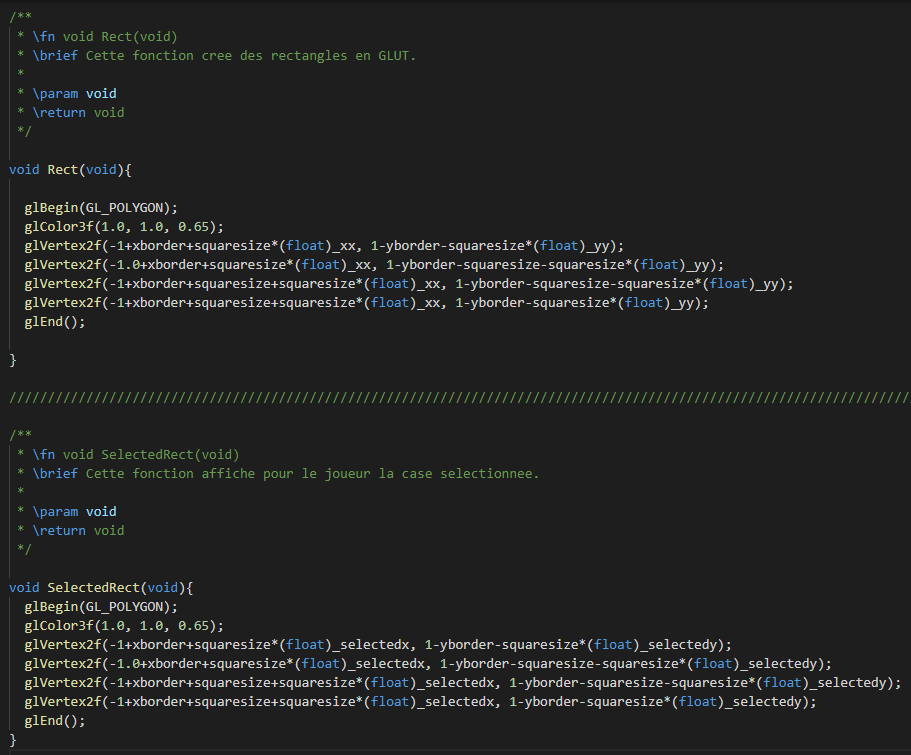
\includegraphics[width = 8cm, height = 5cm]{fact_avant.png}
\bigbreak

\large\bf{Après :}
\bigbreak
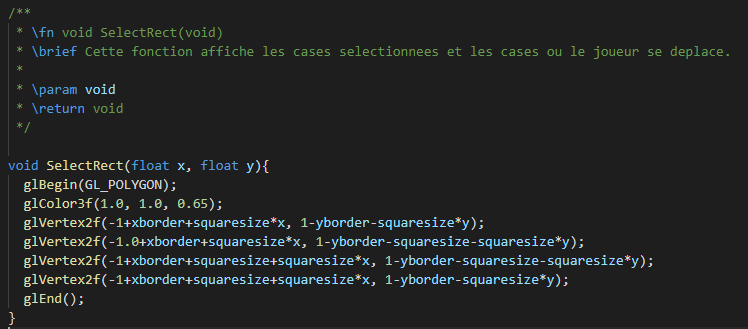
\includegraphics[width = 8cm, height = 5cm]{fact_new.png}

\begin{verbatim}

La nouvelle fonction SelectRect() a remplace les deux fonctions Rect() et SelectedRect().
Cette fonction SelectRect() est responsable de l'affichage des cases selectionnées et les 
cases qui indique le deplacement par boutons fleches du joueur sur le plateau. Elle prend 
deux floats comme argument, et ensuite elle modifie les valuers des variables globales.
Avant cette factorisation, les deux fonctions  Rect() et SelectedRect() s'occupaient des 
la case selectionnee et de la case de deplacement par fleche separemment.

Concernant la factorisation du reste de notre code, nous avons corrigé au fur et à 
mesure ces divers éléments afin de rendre le code plus limpide et efficace. Nous avons 
fait de notre mieux pour optimiser et organiser de manière efficace notre programme dès 
le départ.De plus, le fait d'utiliser le GLUT ne permet pas une factorisation facile 
d'approche car nous ne pouvons pas prendre des arguments en paramètre de nos fonctions.


\end{verbatim}

\bigbreak
\bigbreak
\bigbreak
\bigbreak
\bigbreak
\bigbreak
\bigbreak
\bigbreak
\bigbreak
\bigbreak
\bigbreak
\bigbreak
\bigbreak
\bigbreak
\bigbreak
\bigbreak
\bigbreak
\bigbreak
\bigbreak
\bigbreak
\bigbreak
\bigbreak
\bigbreak

\section{Exécution du programme}


\large\bf{Début de jeu :}
\bigbreak

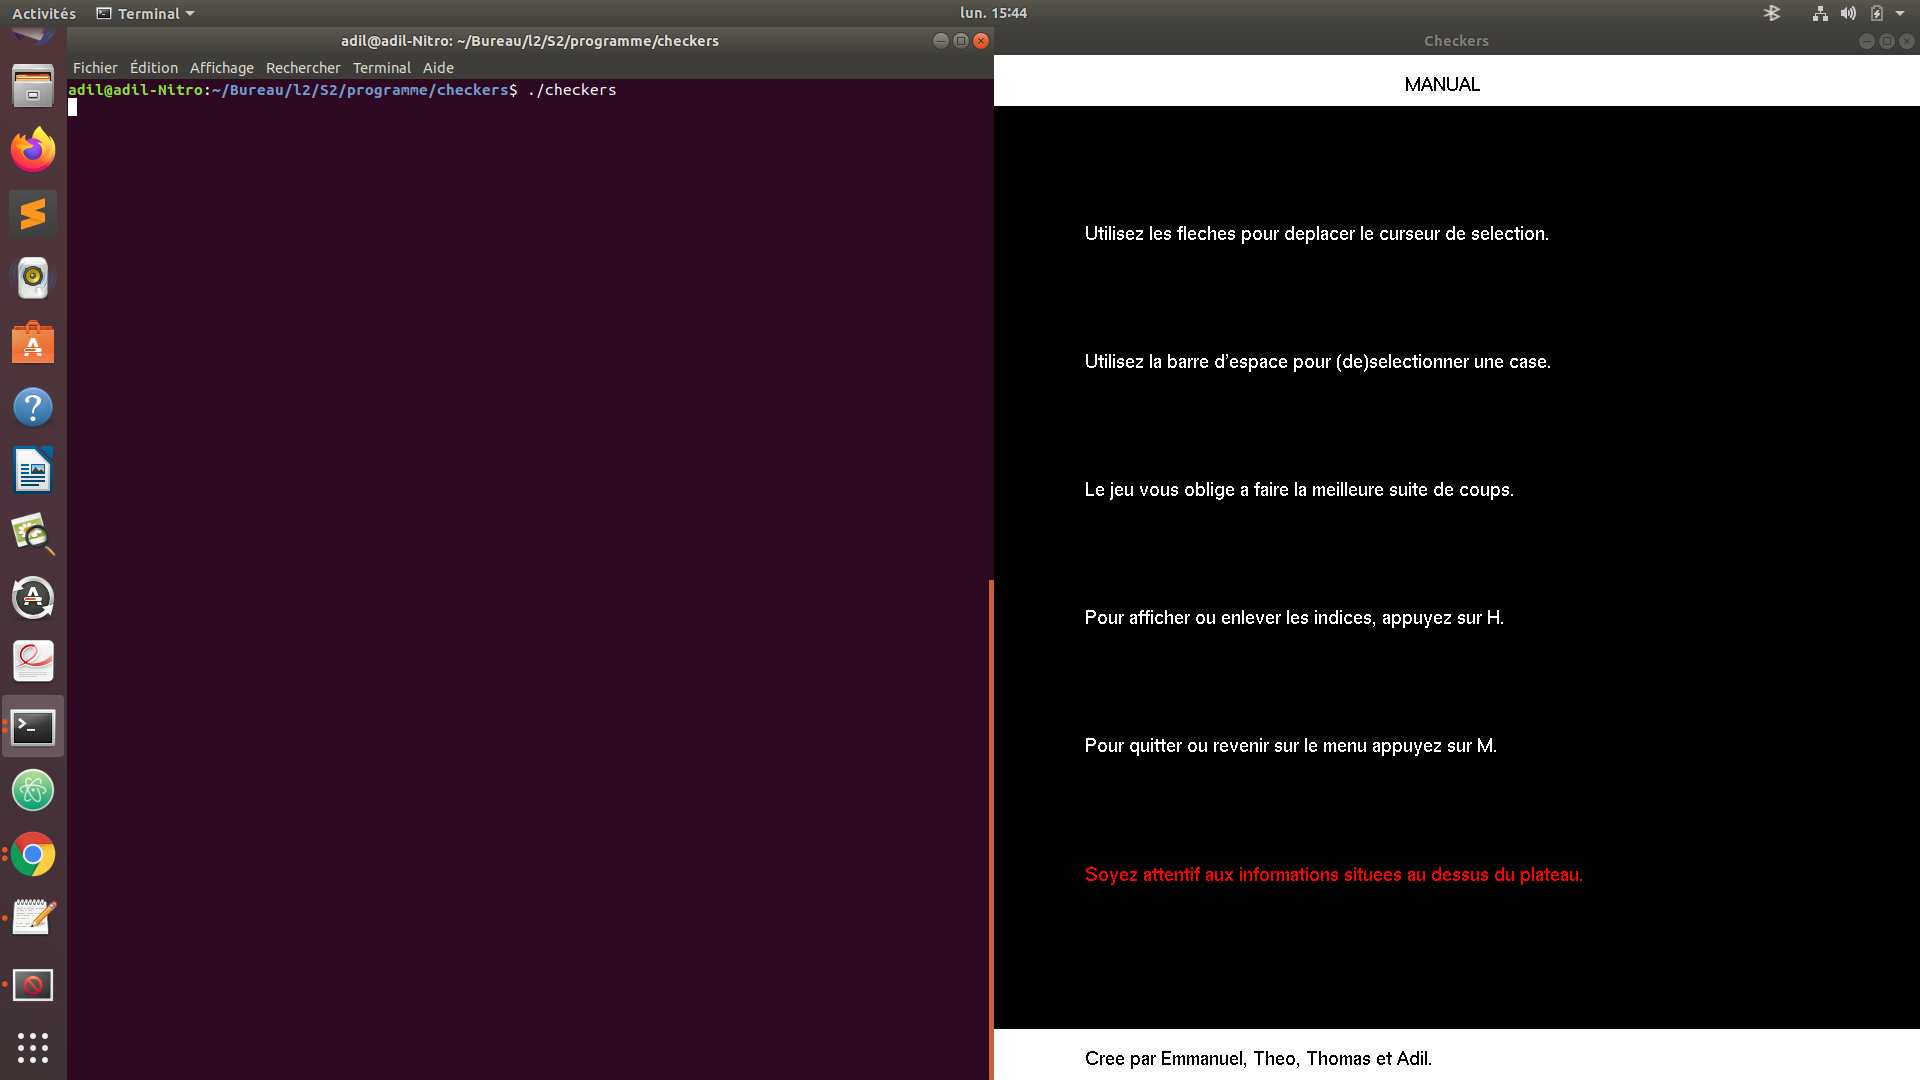
\includegraphics[width = 8cm, height = 5cm]{menu.png}
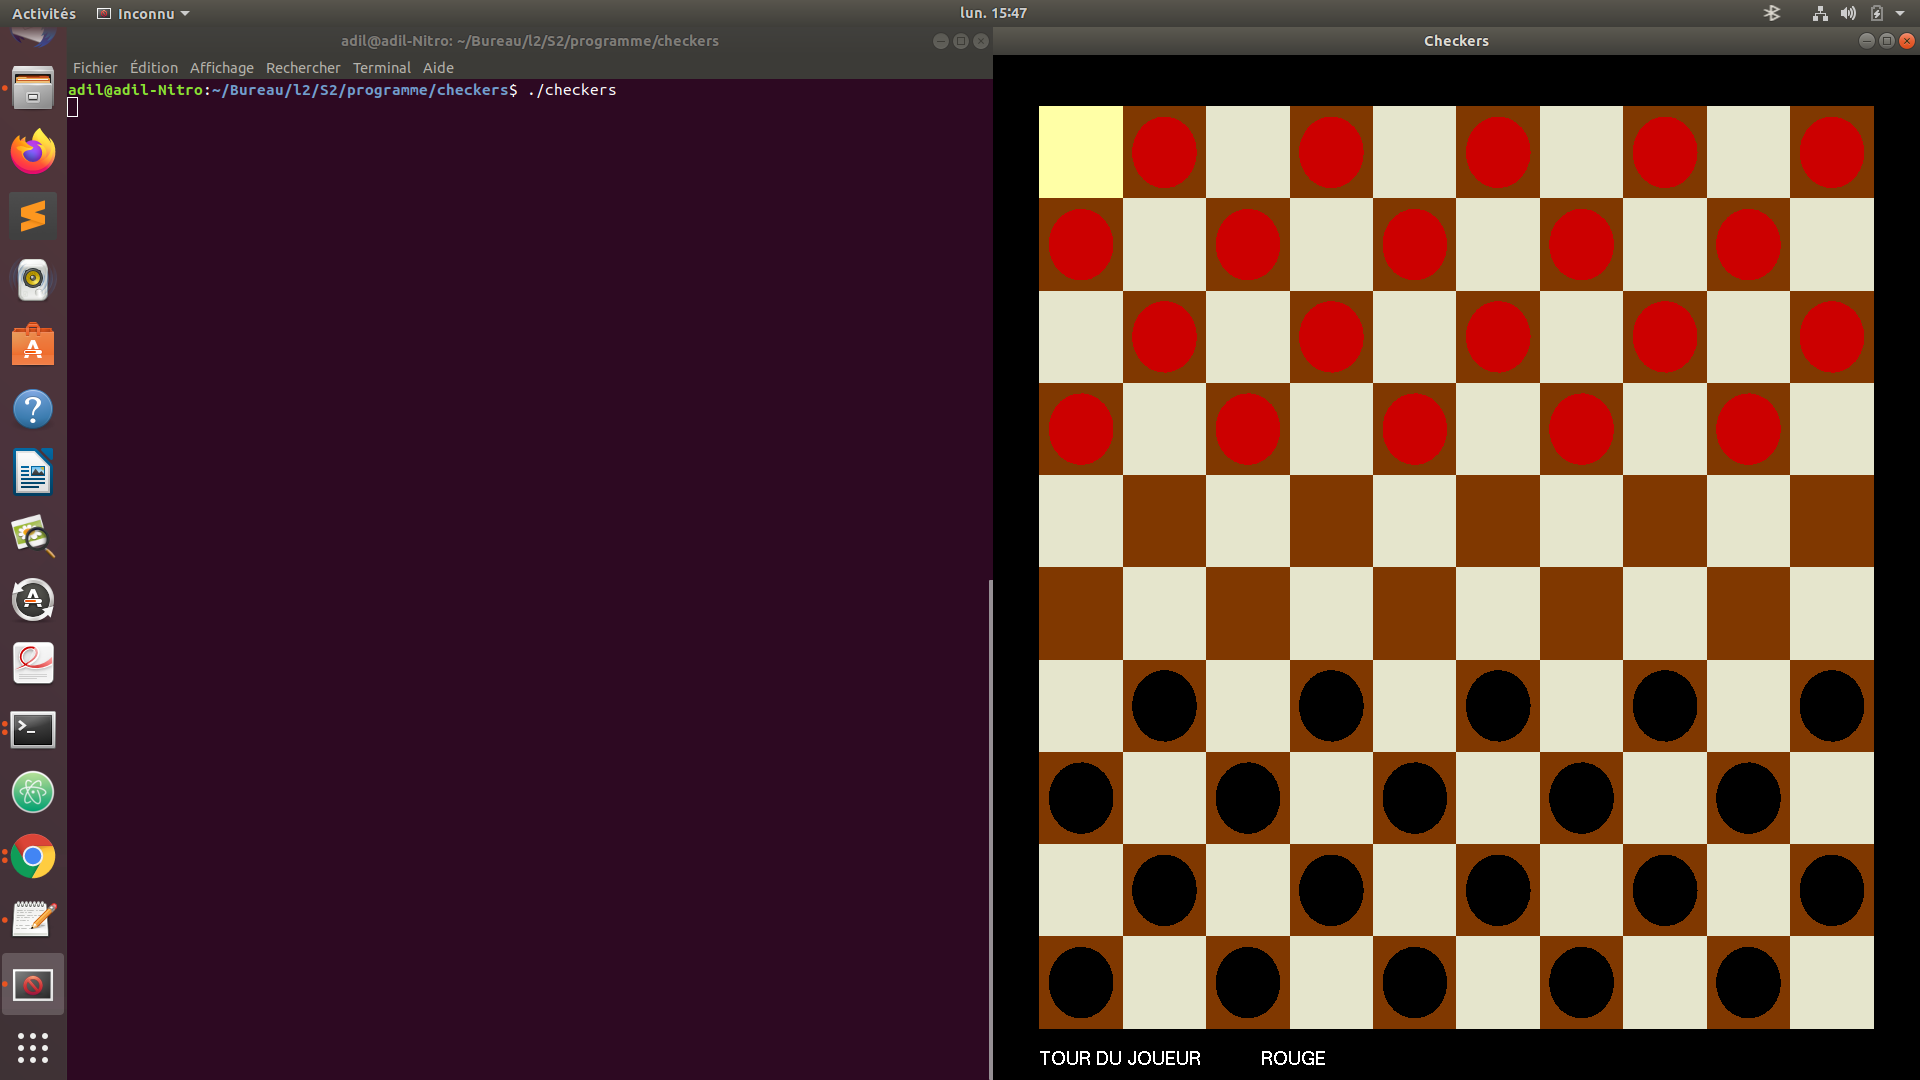
\includegraphics[width = 8cm, height = 5cm]{premiertour1.png}
\bigbreak
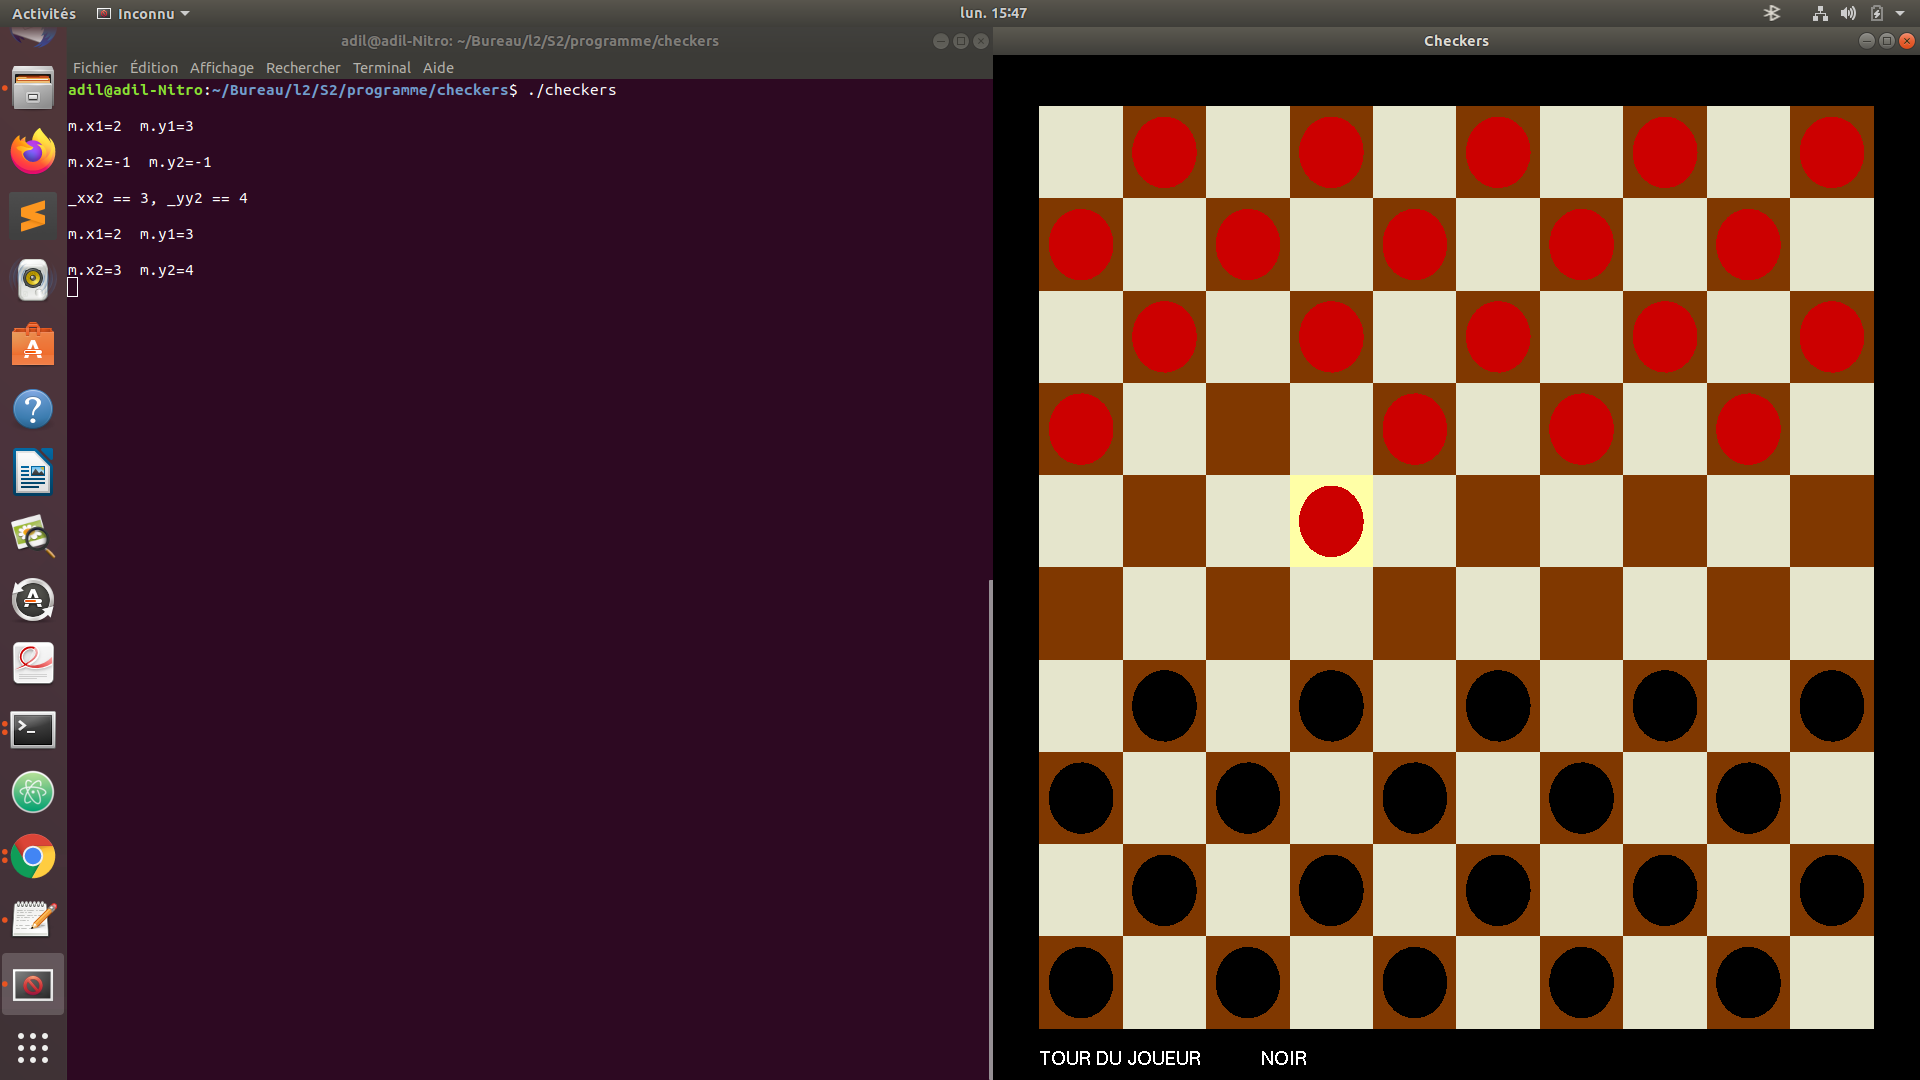
\includegraphics[width = 8cm, height = 5cm]{premiertour2.png}
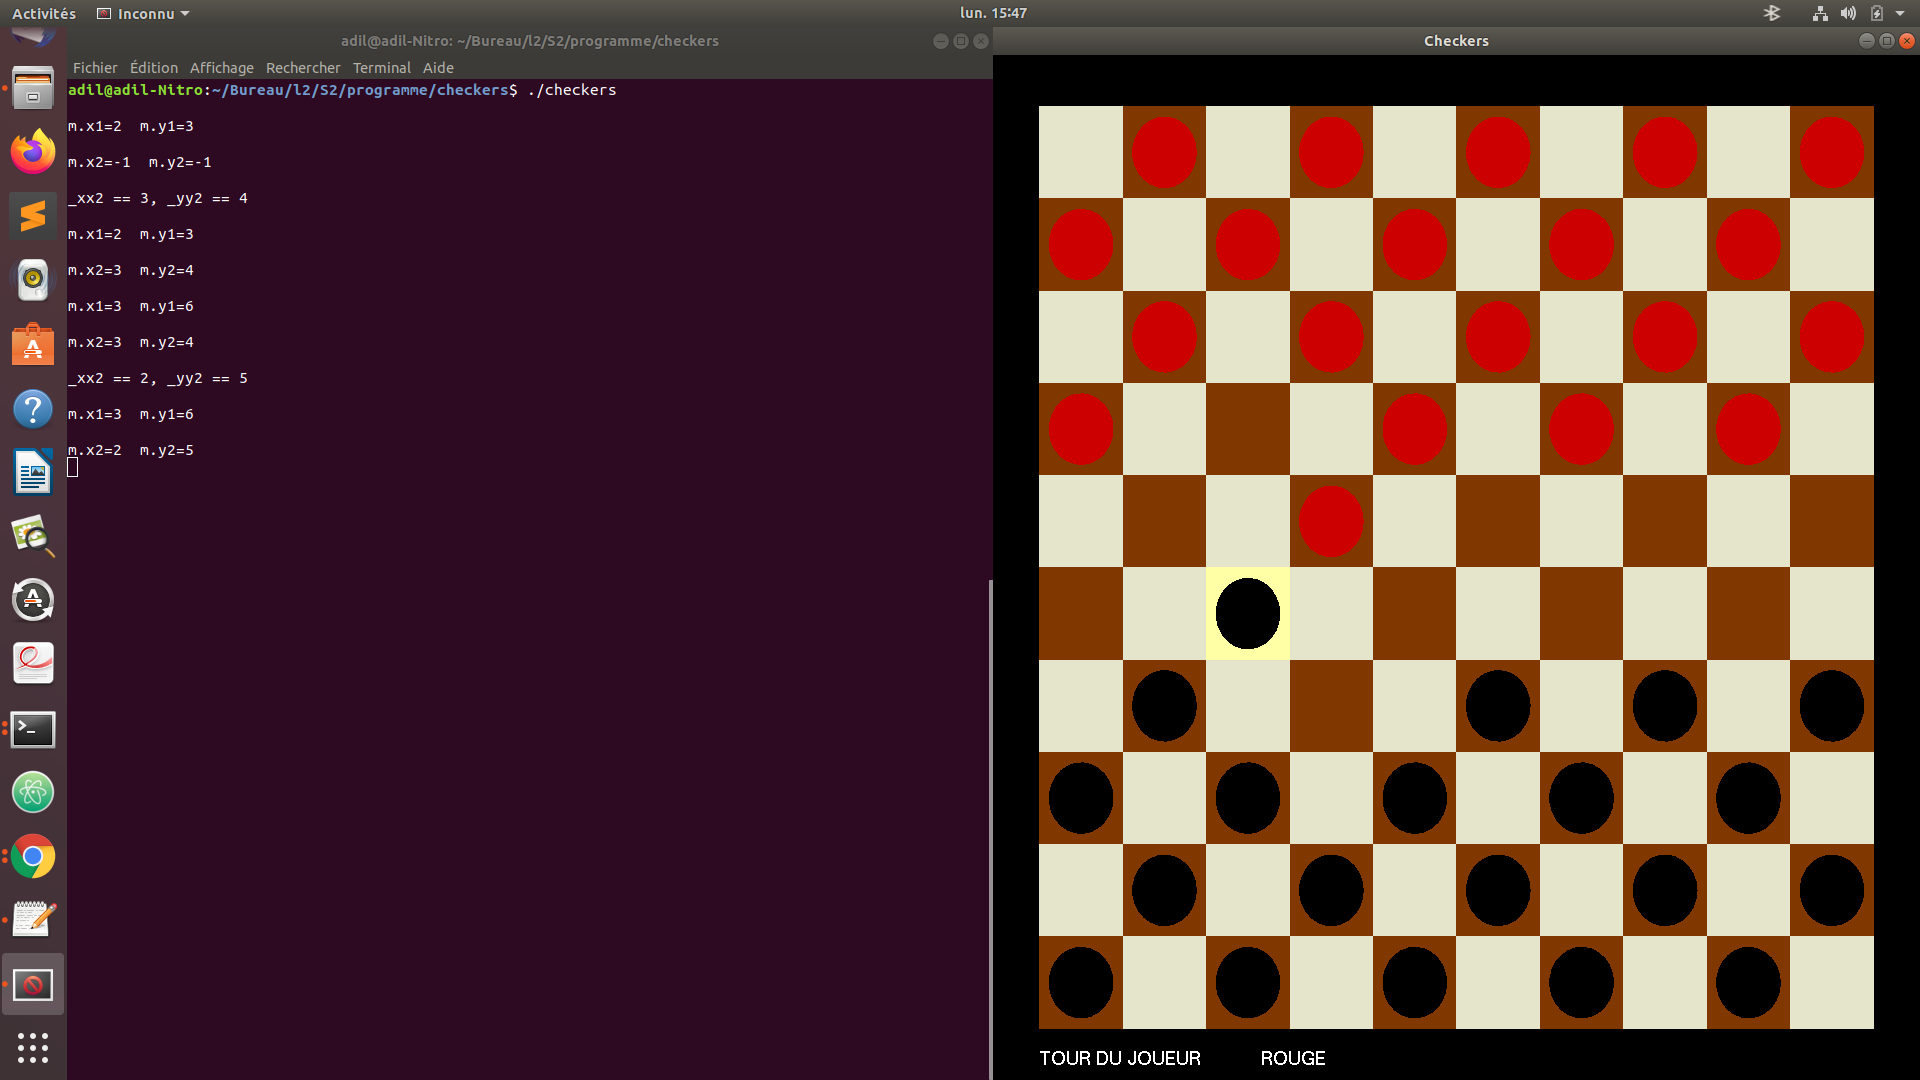
\includegraphics[width = 8cm, height = 5cm]{premiertour3.png}
\bigbreak
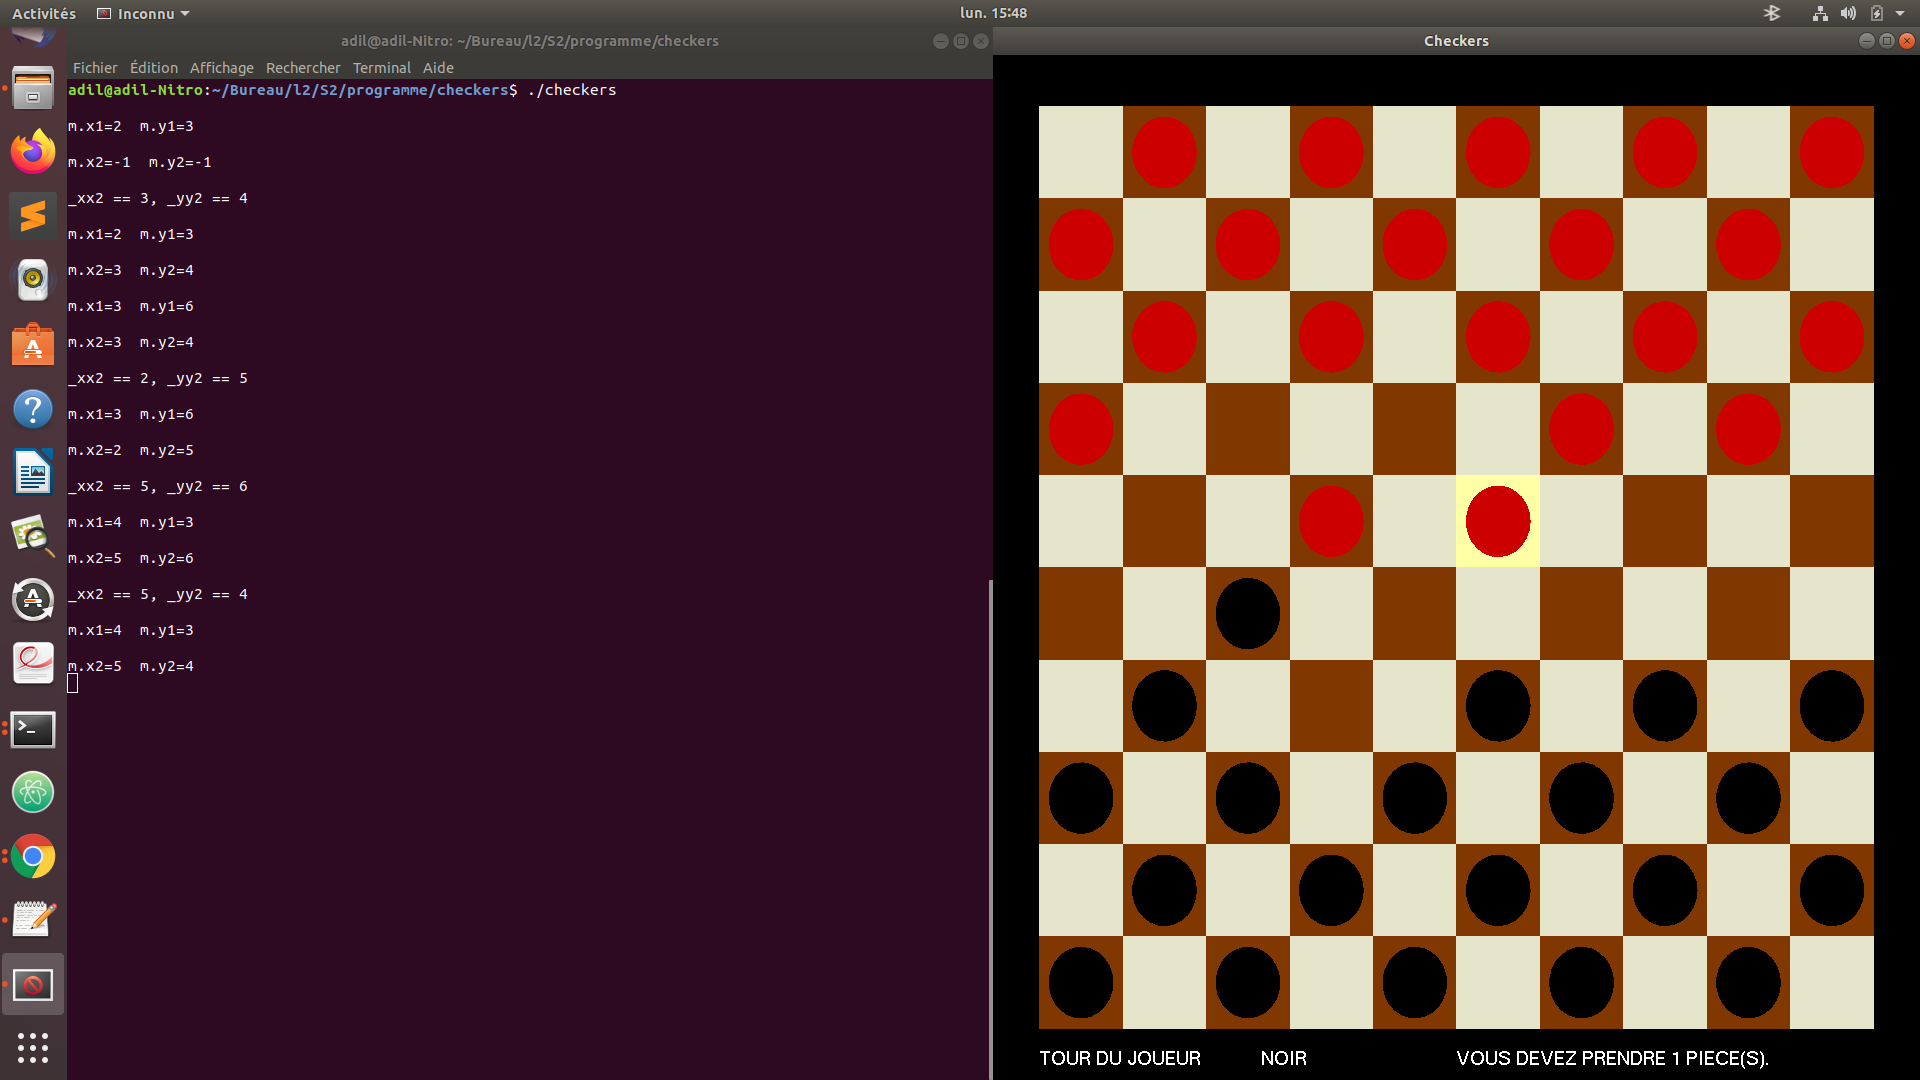
\includegraphics[width = 8cm, height = 5cm]{premiertour4.png}
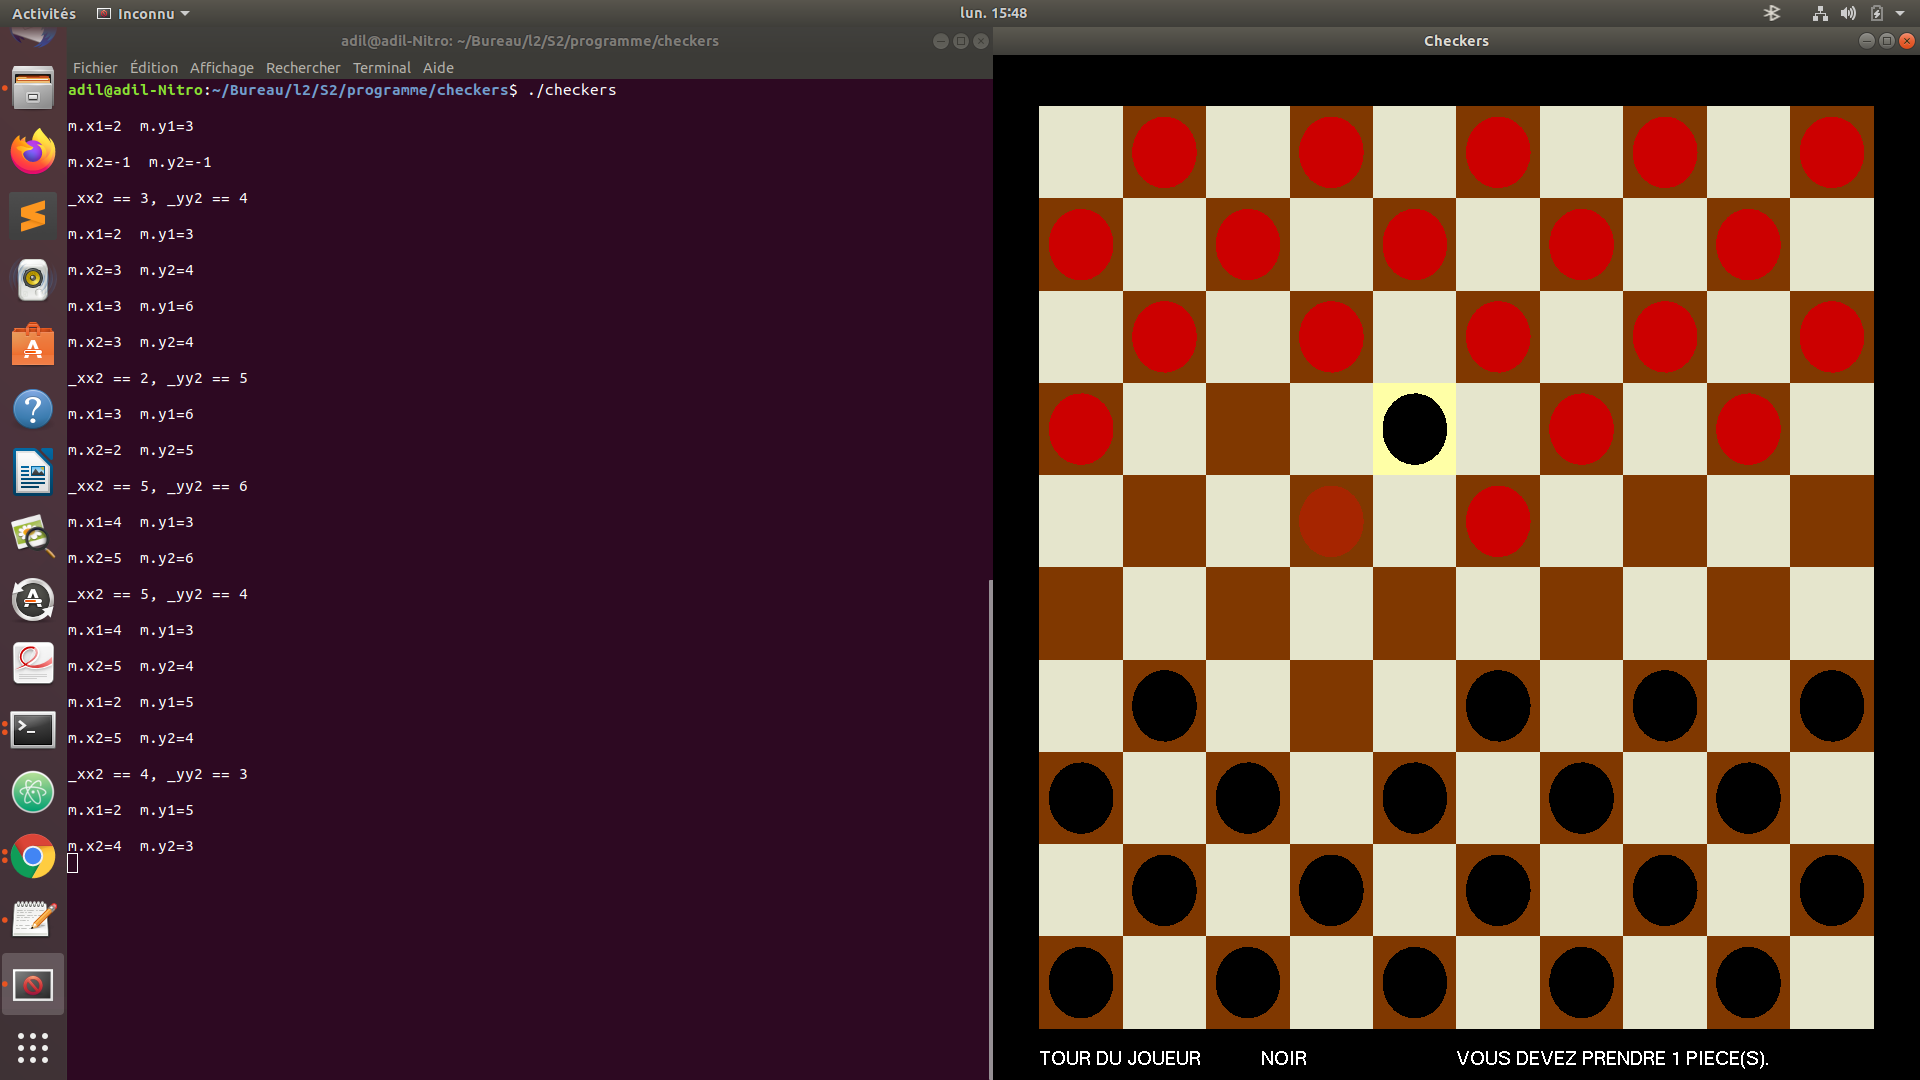
\includegraphics[width = 8cm, height = 5cm]{premiertour5.png}
\bigbreak
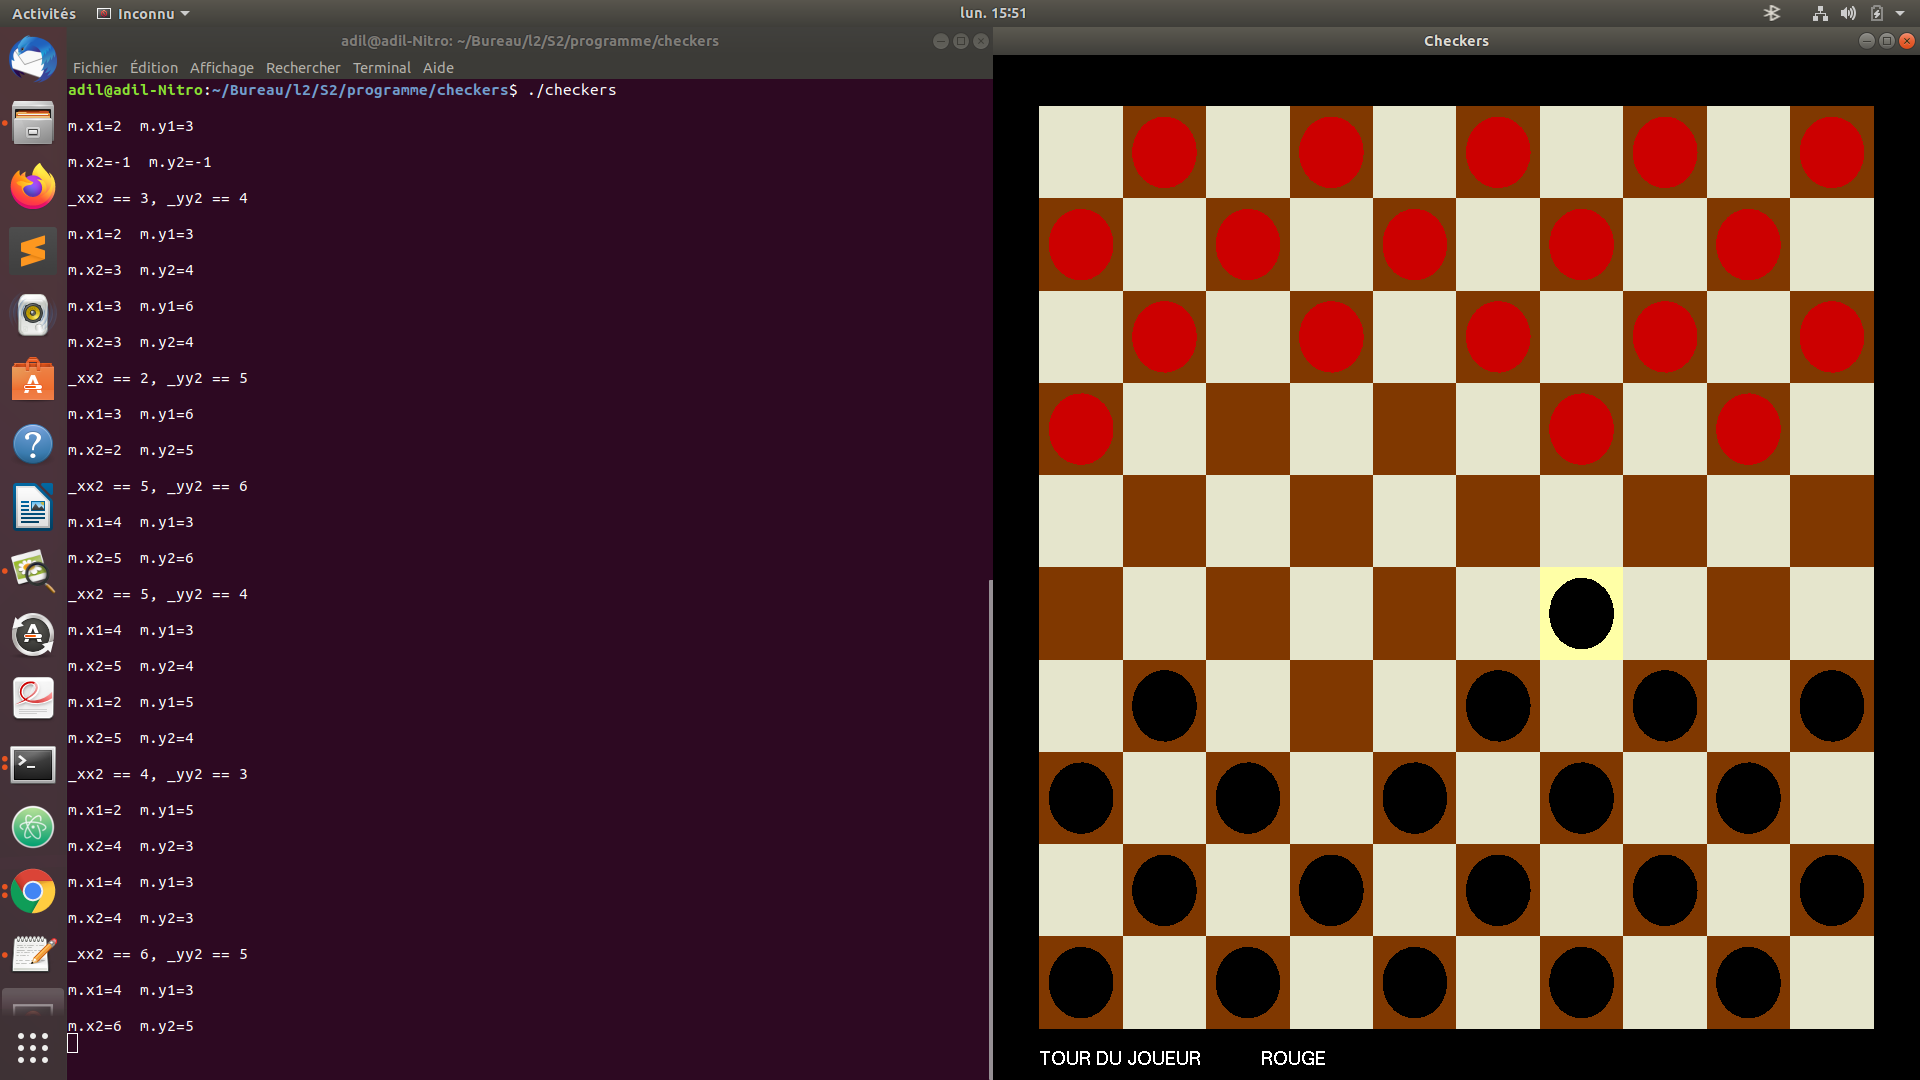
\includegraphics[width = 8cm, height = 5cm]{premiertour6.png}
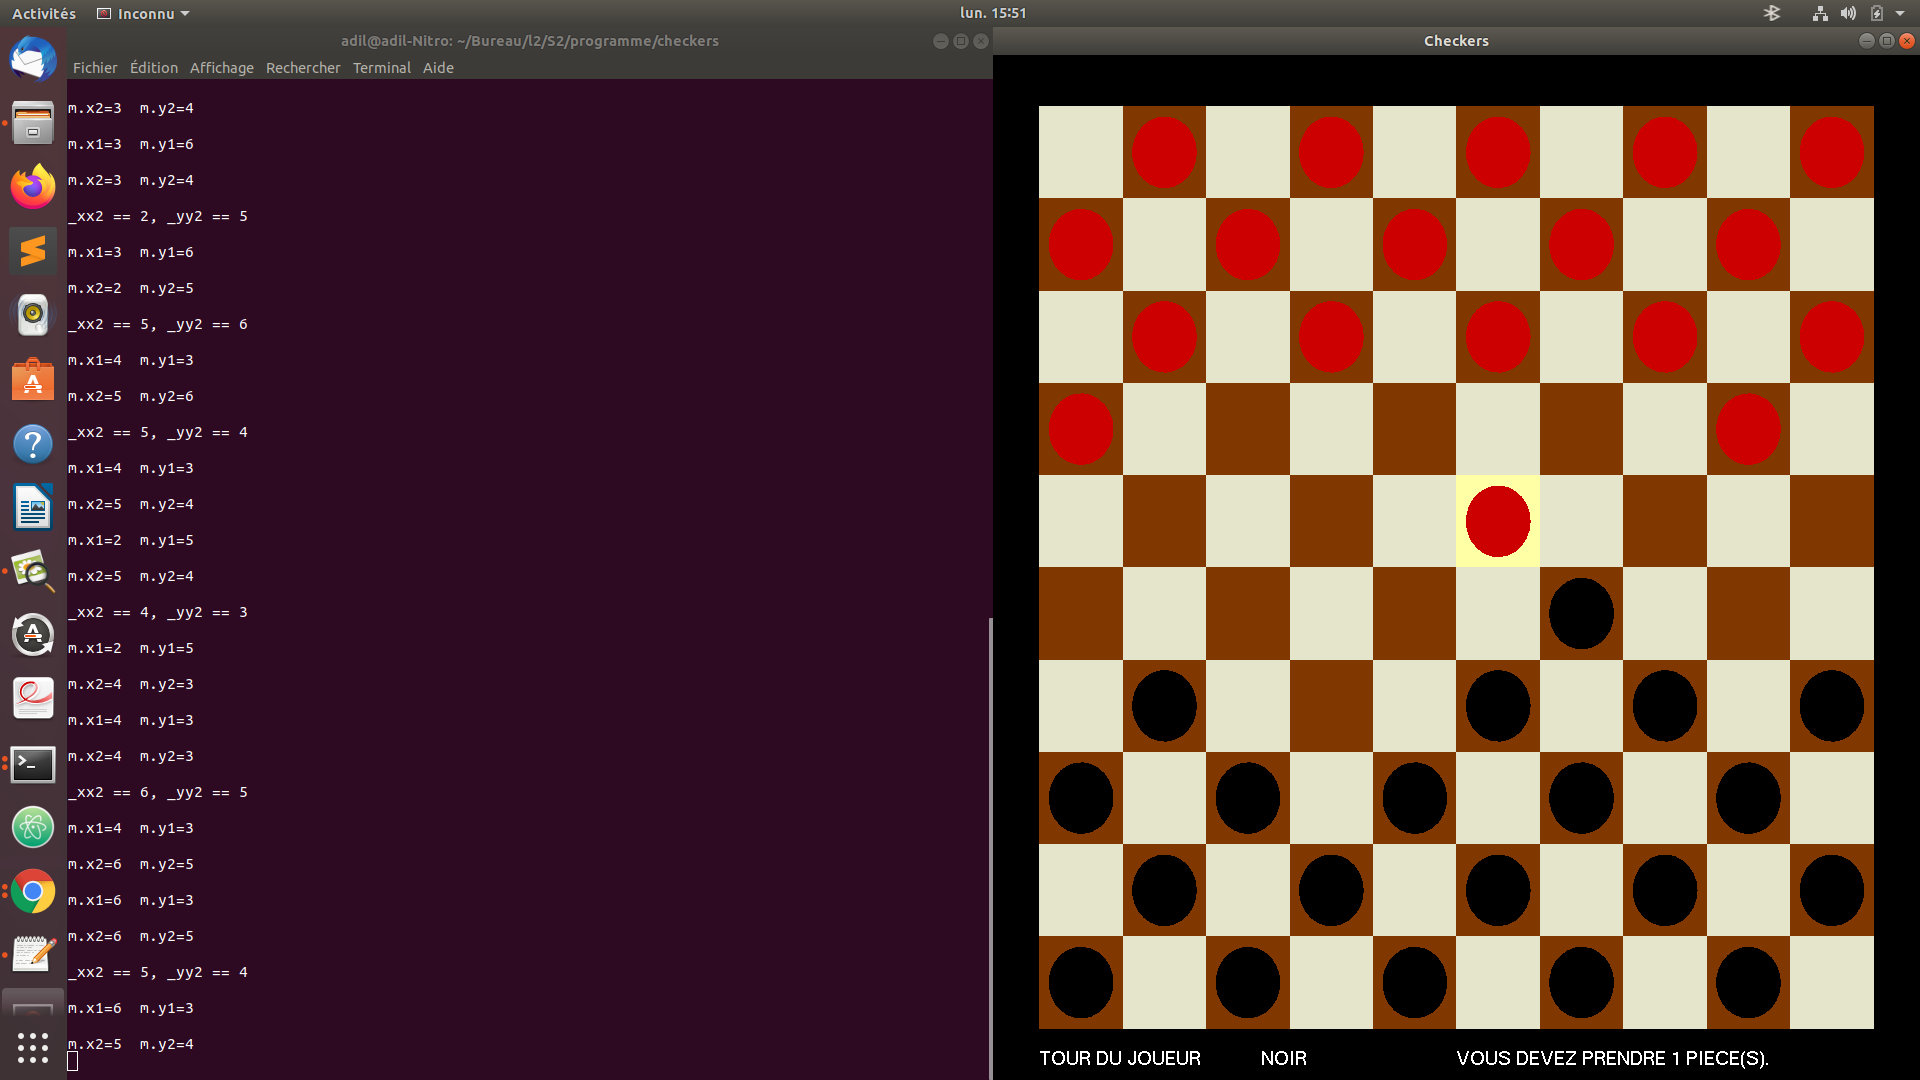
\includegraphics[width = 8cm, height = 5cm]{premiertour7.png}
\bigbreak
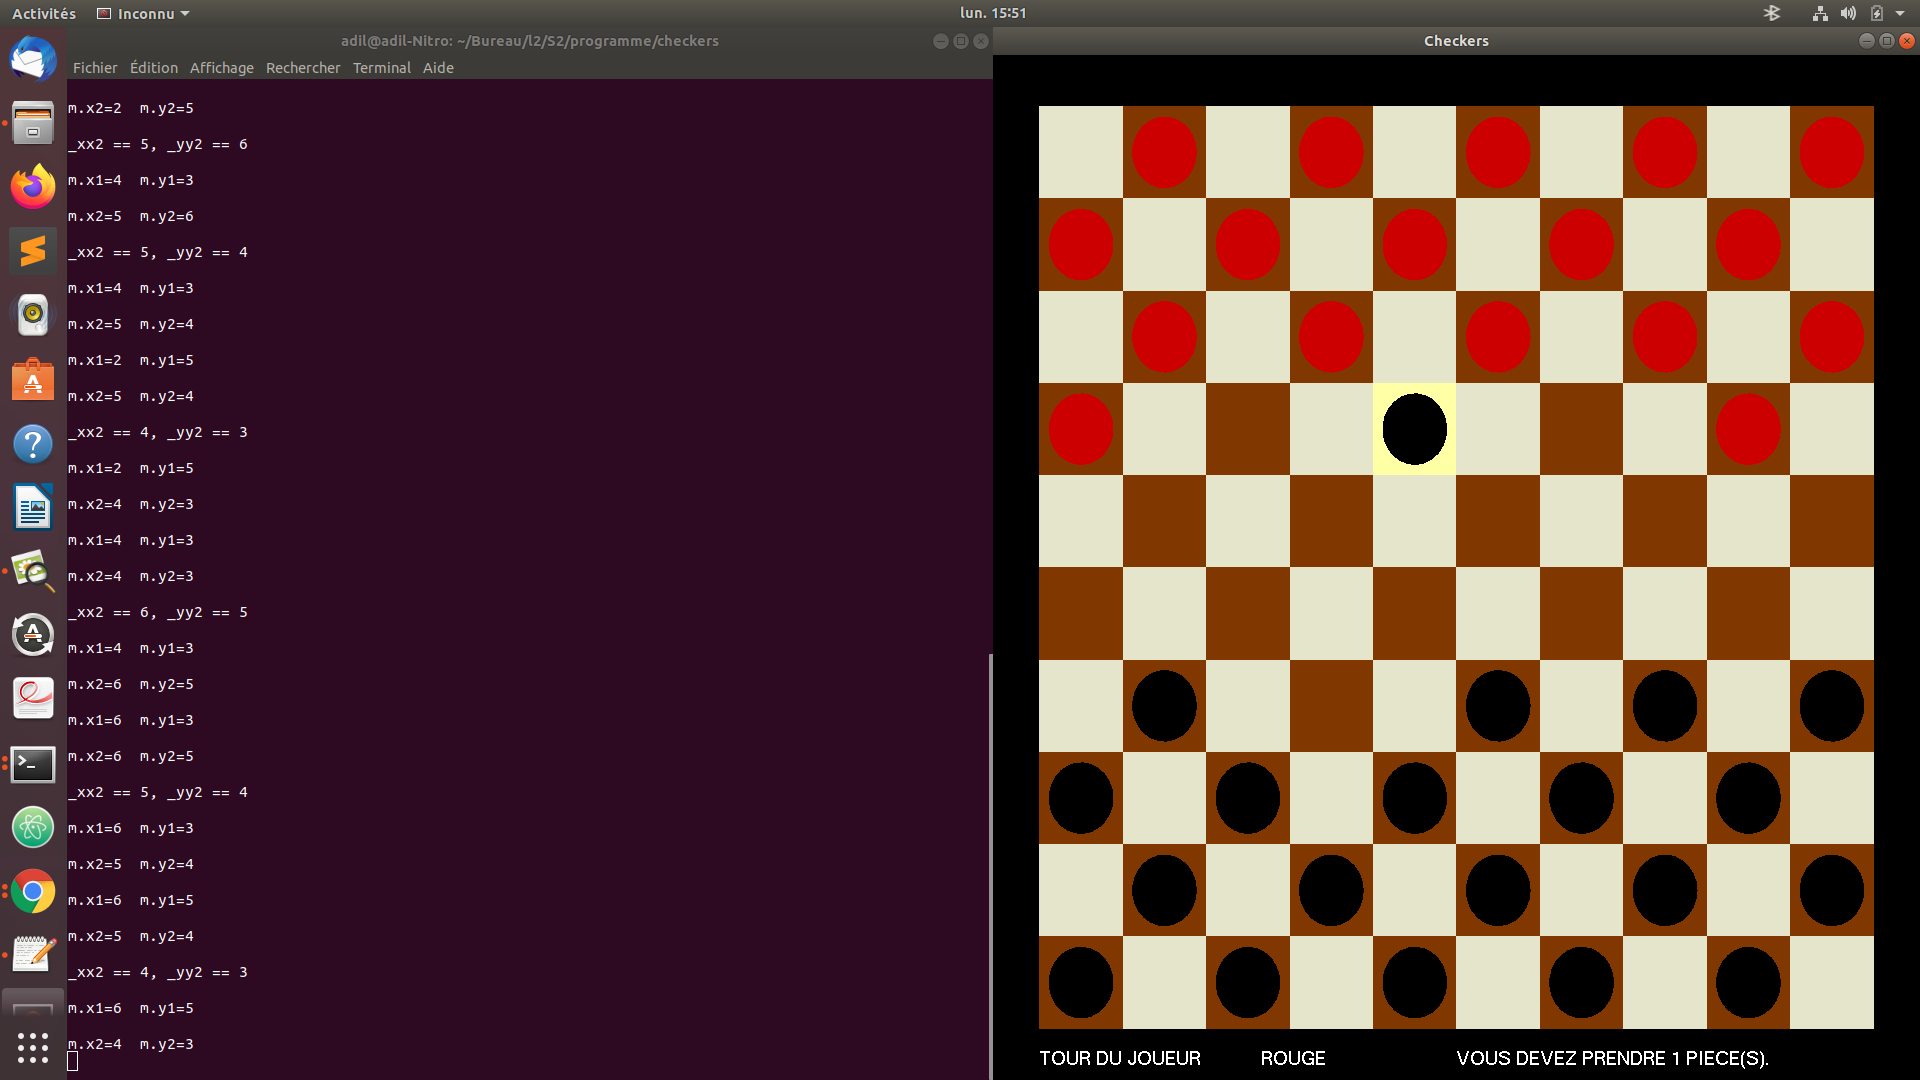
\includegraphics[width = 8cm, height = 5cm]{premiertour8.png}
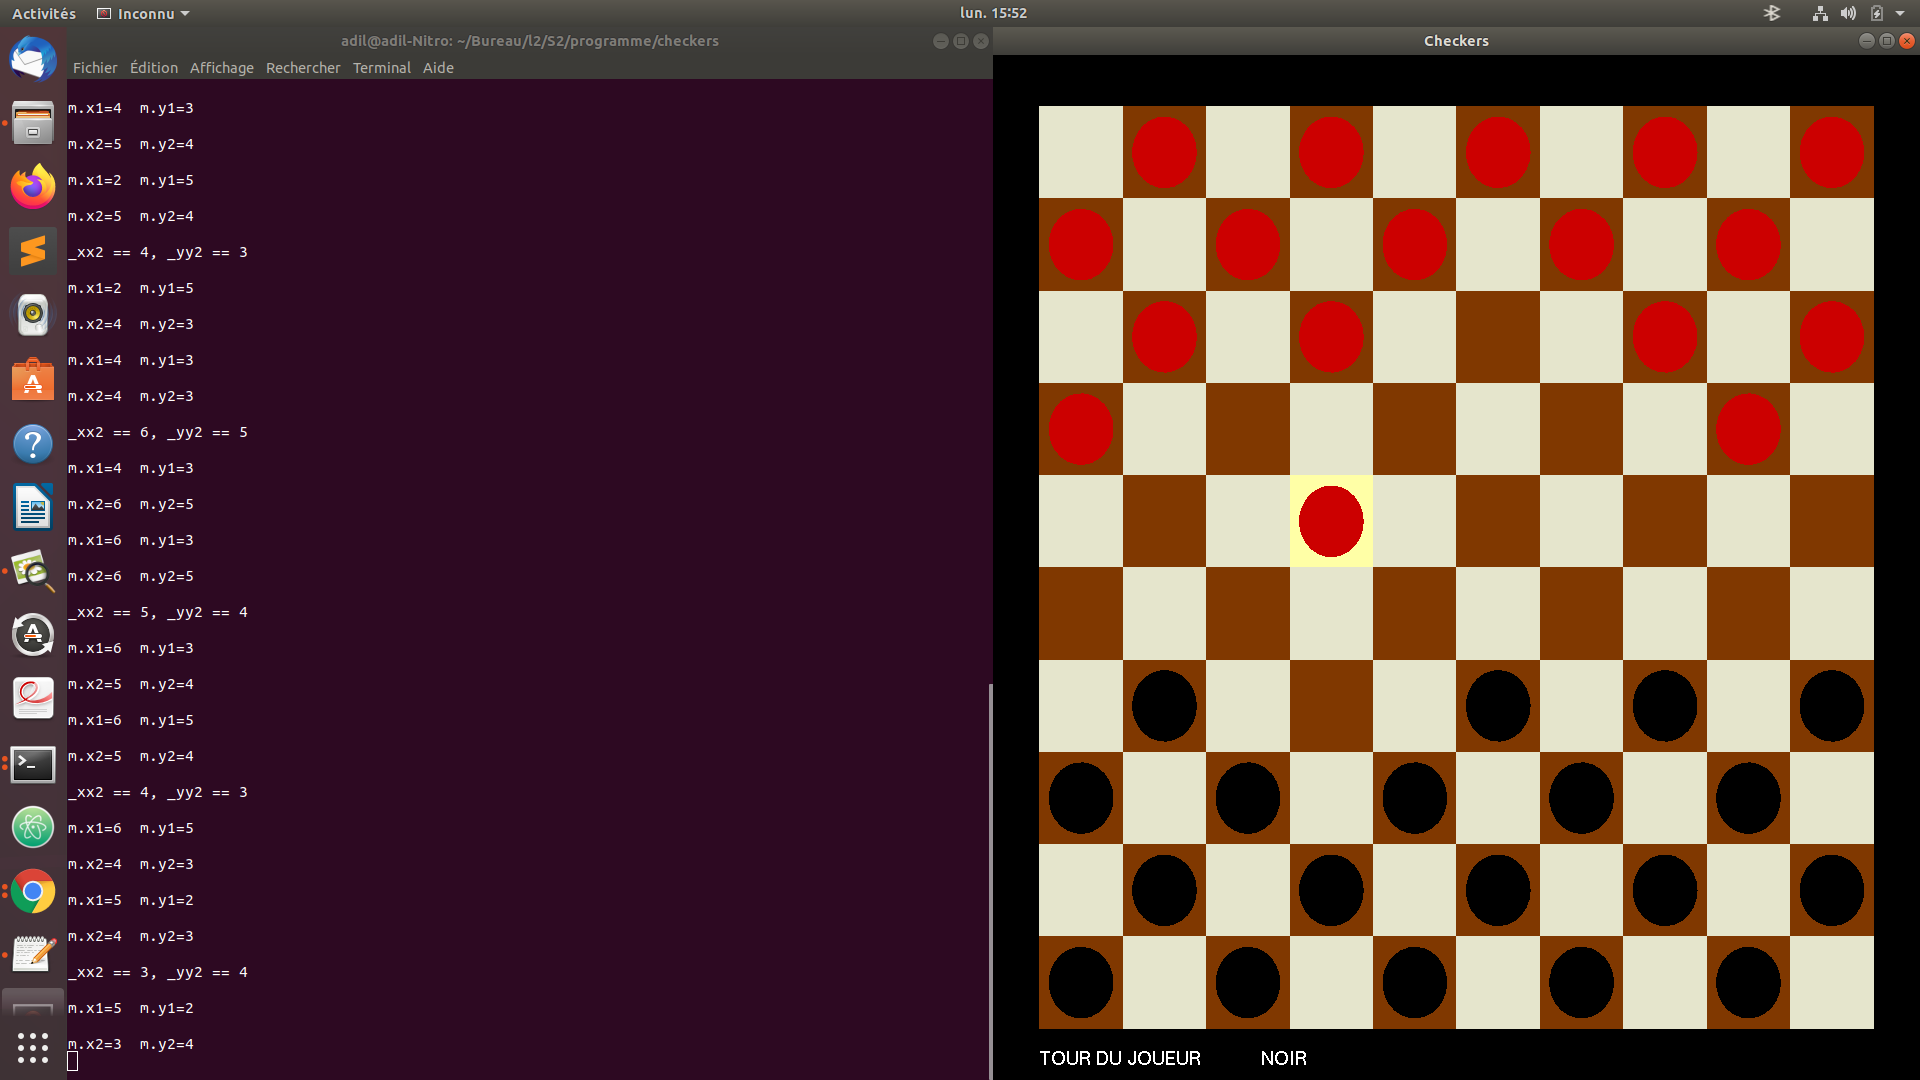
\includegraphics[width = 8cm, height = 5cm]{premiertour9.png}
\bigbreak

\large\bf{Fin de partie (pion) : }
\bigbreak

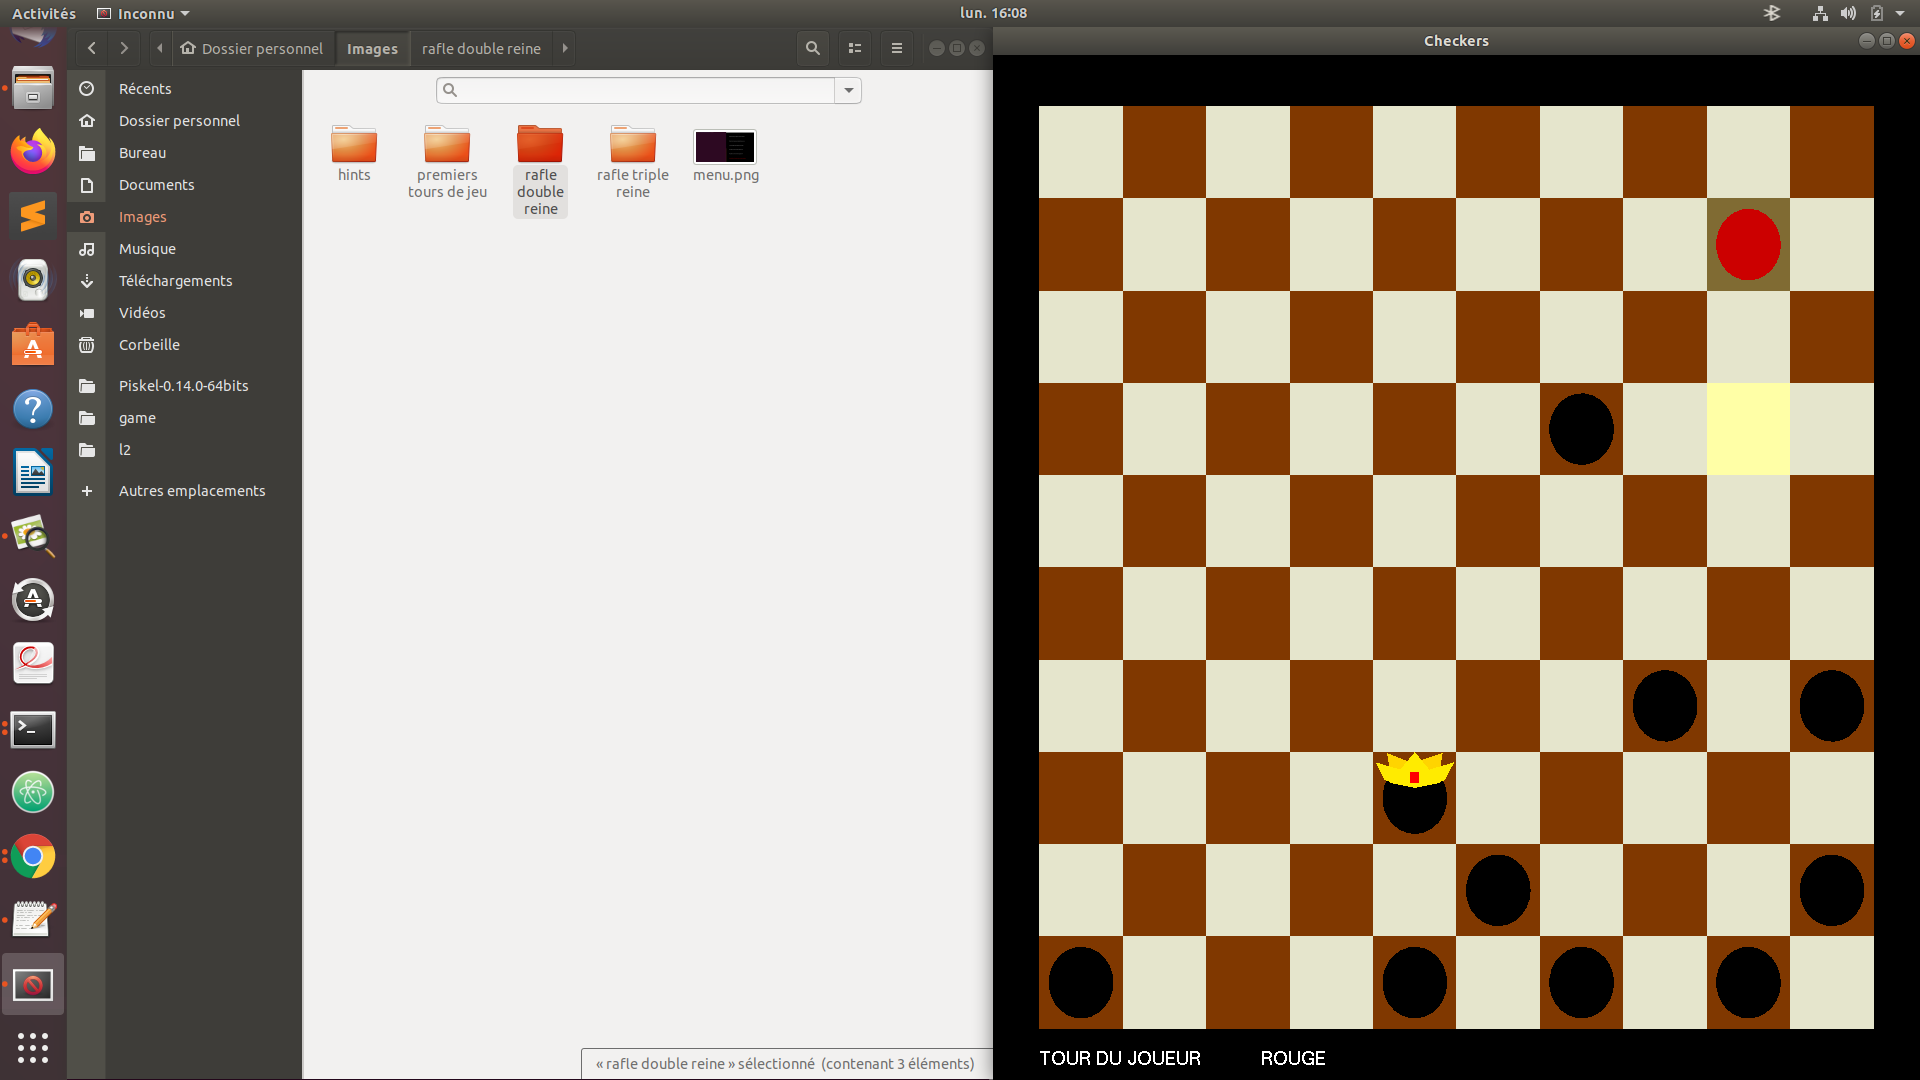
\includegraphics[width = 8cm, height = 5cm]{Pion.png}
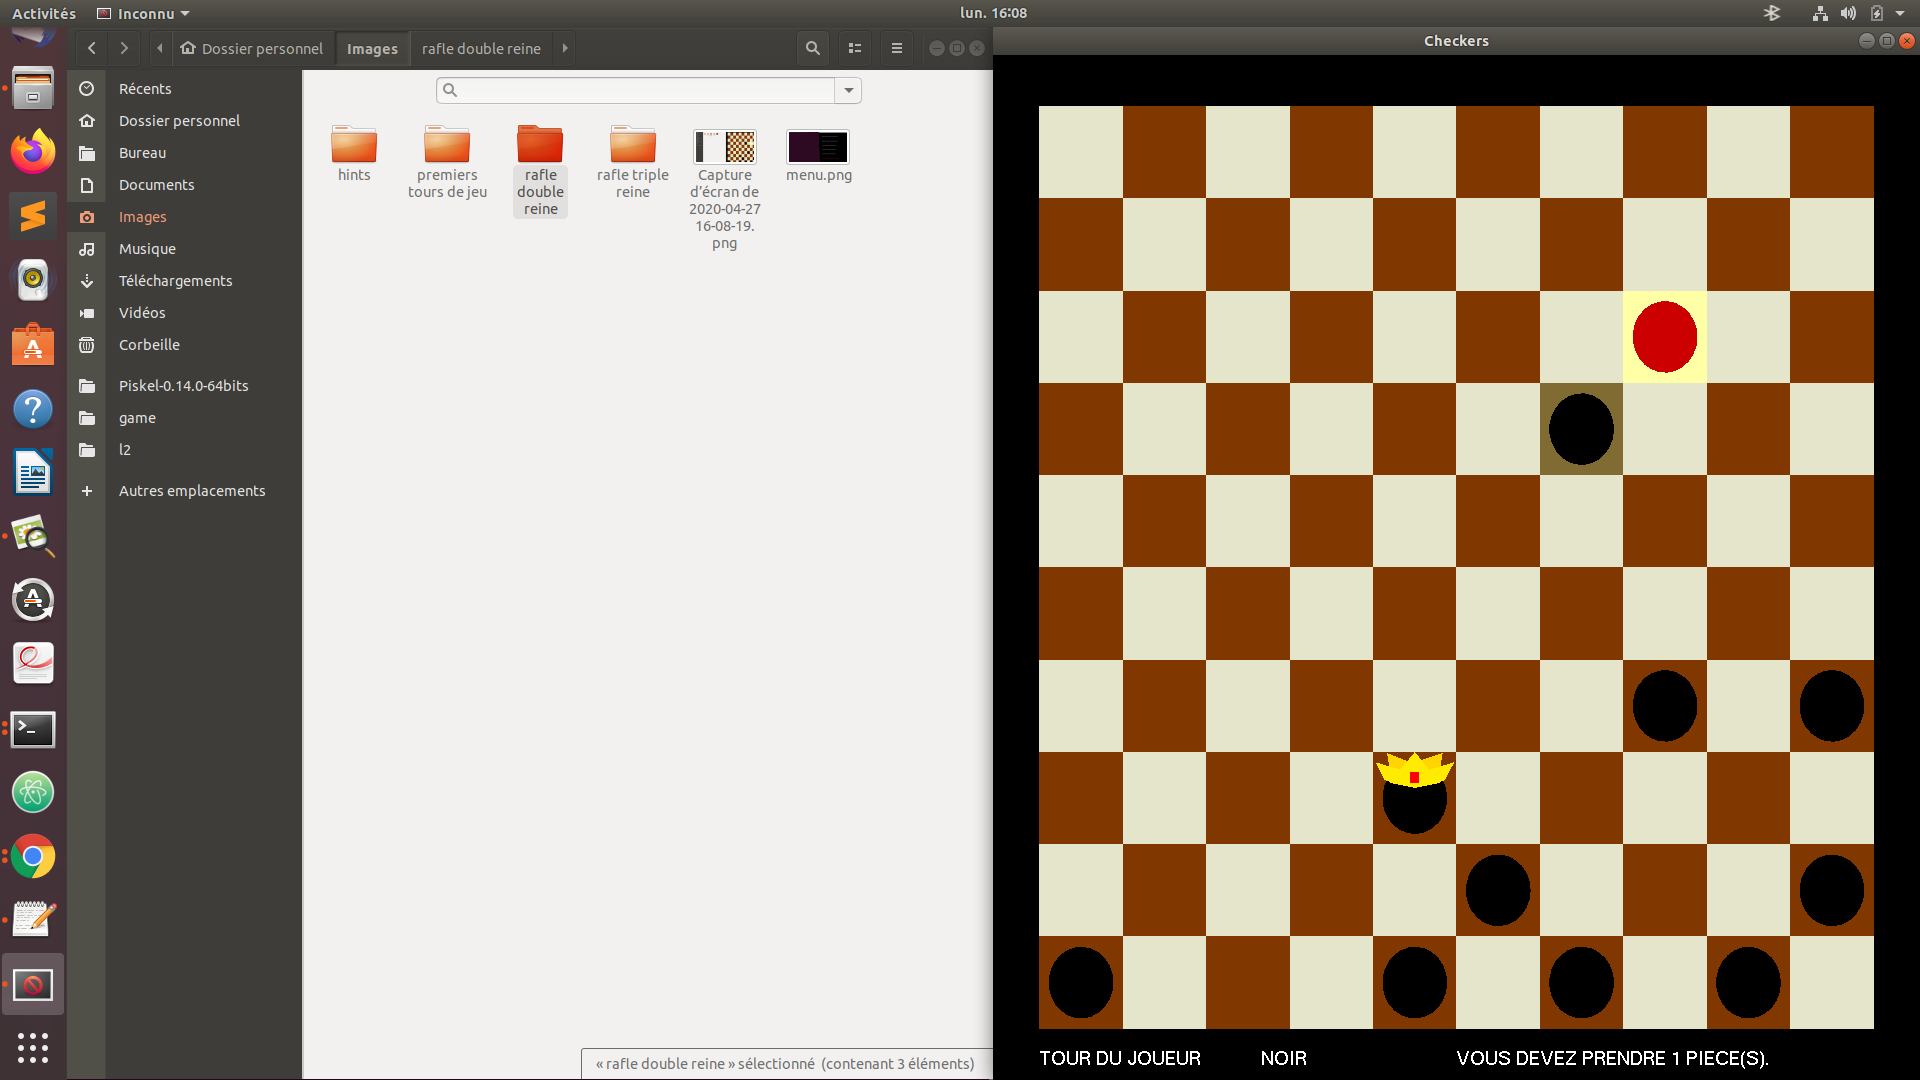
\includegraphics[width = 8cm, height = 5cm]{Pion2.png}
\bigbreak
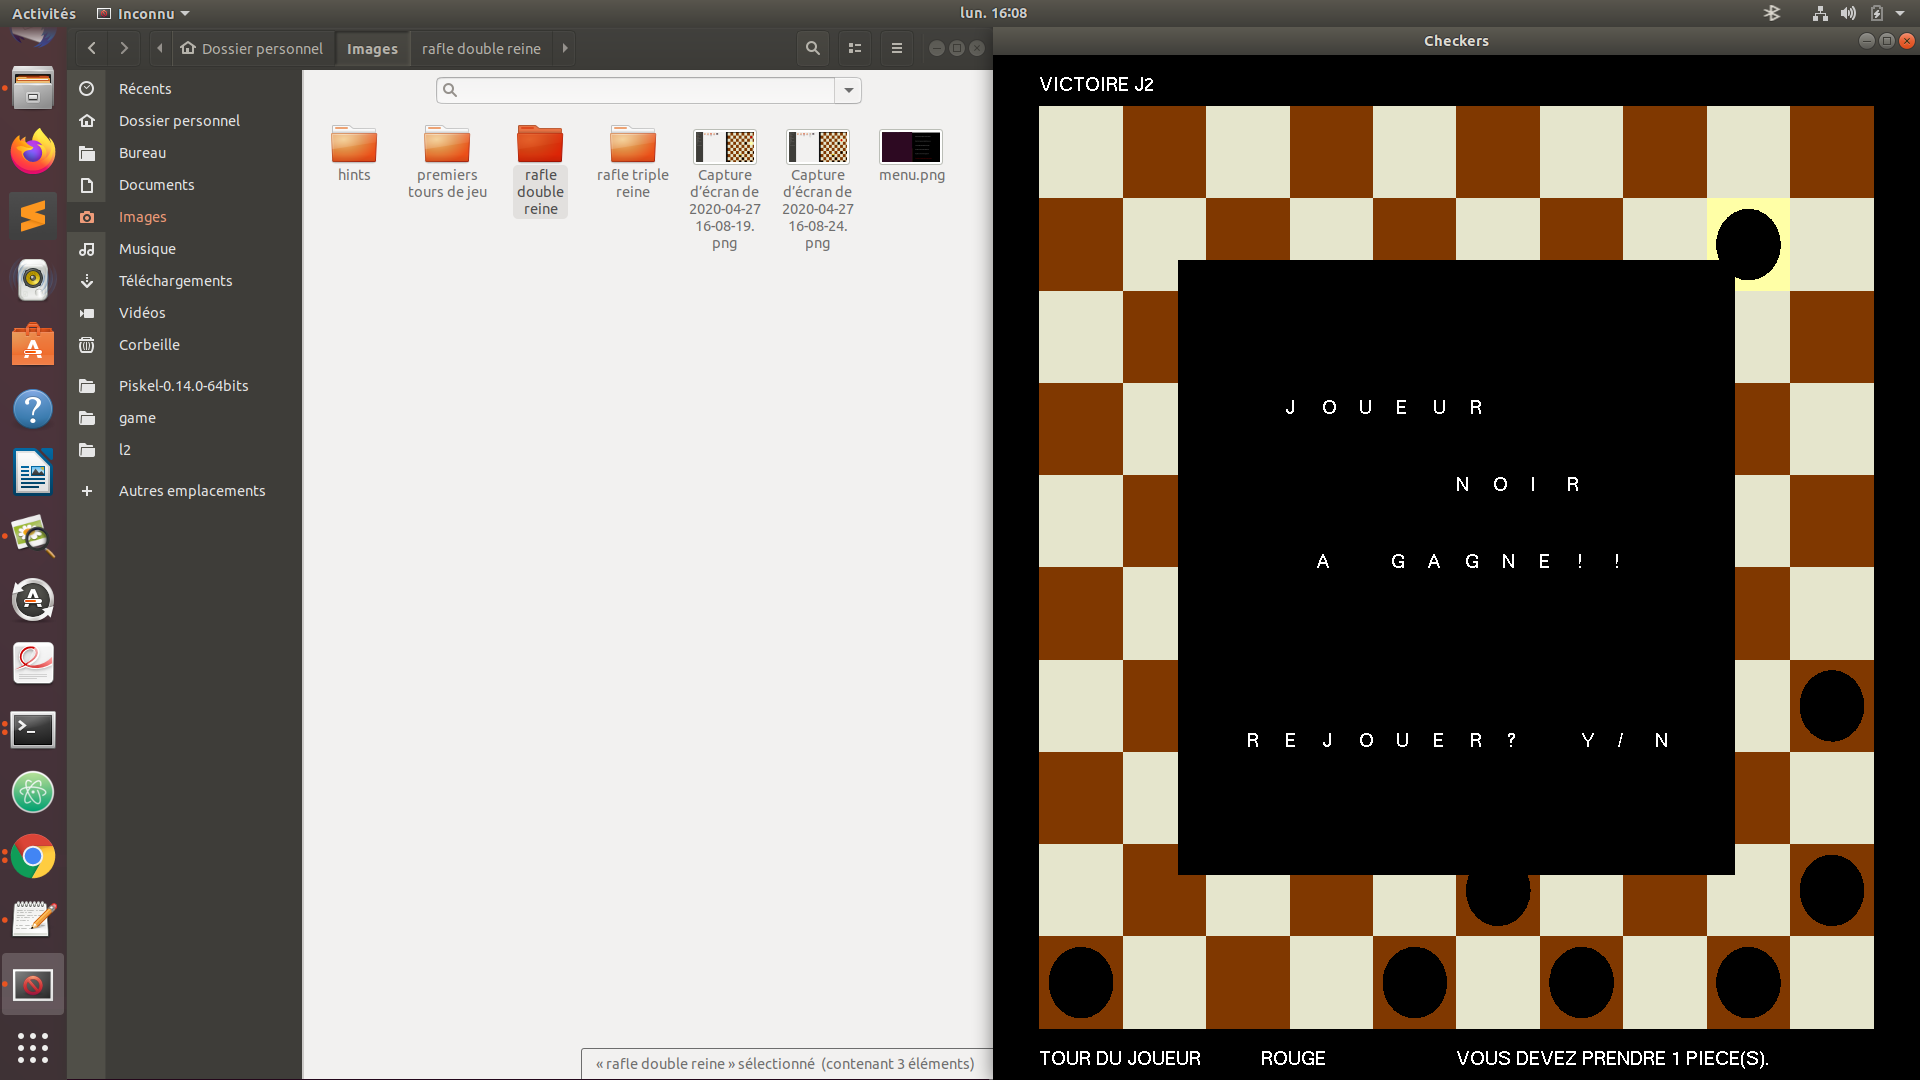
\includegraphics[width = 8cm, height = 5cm]{Pion3.png}

\bigbreak
\large\bf{Fin de partie (reine) : }
\bigbreak

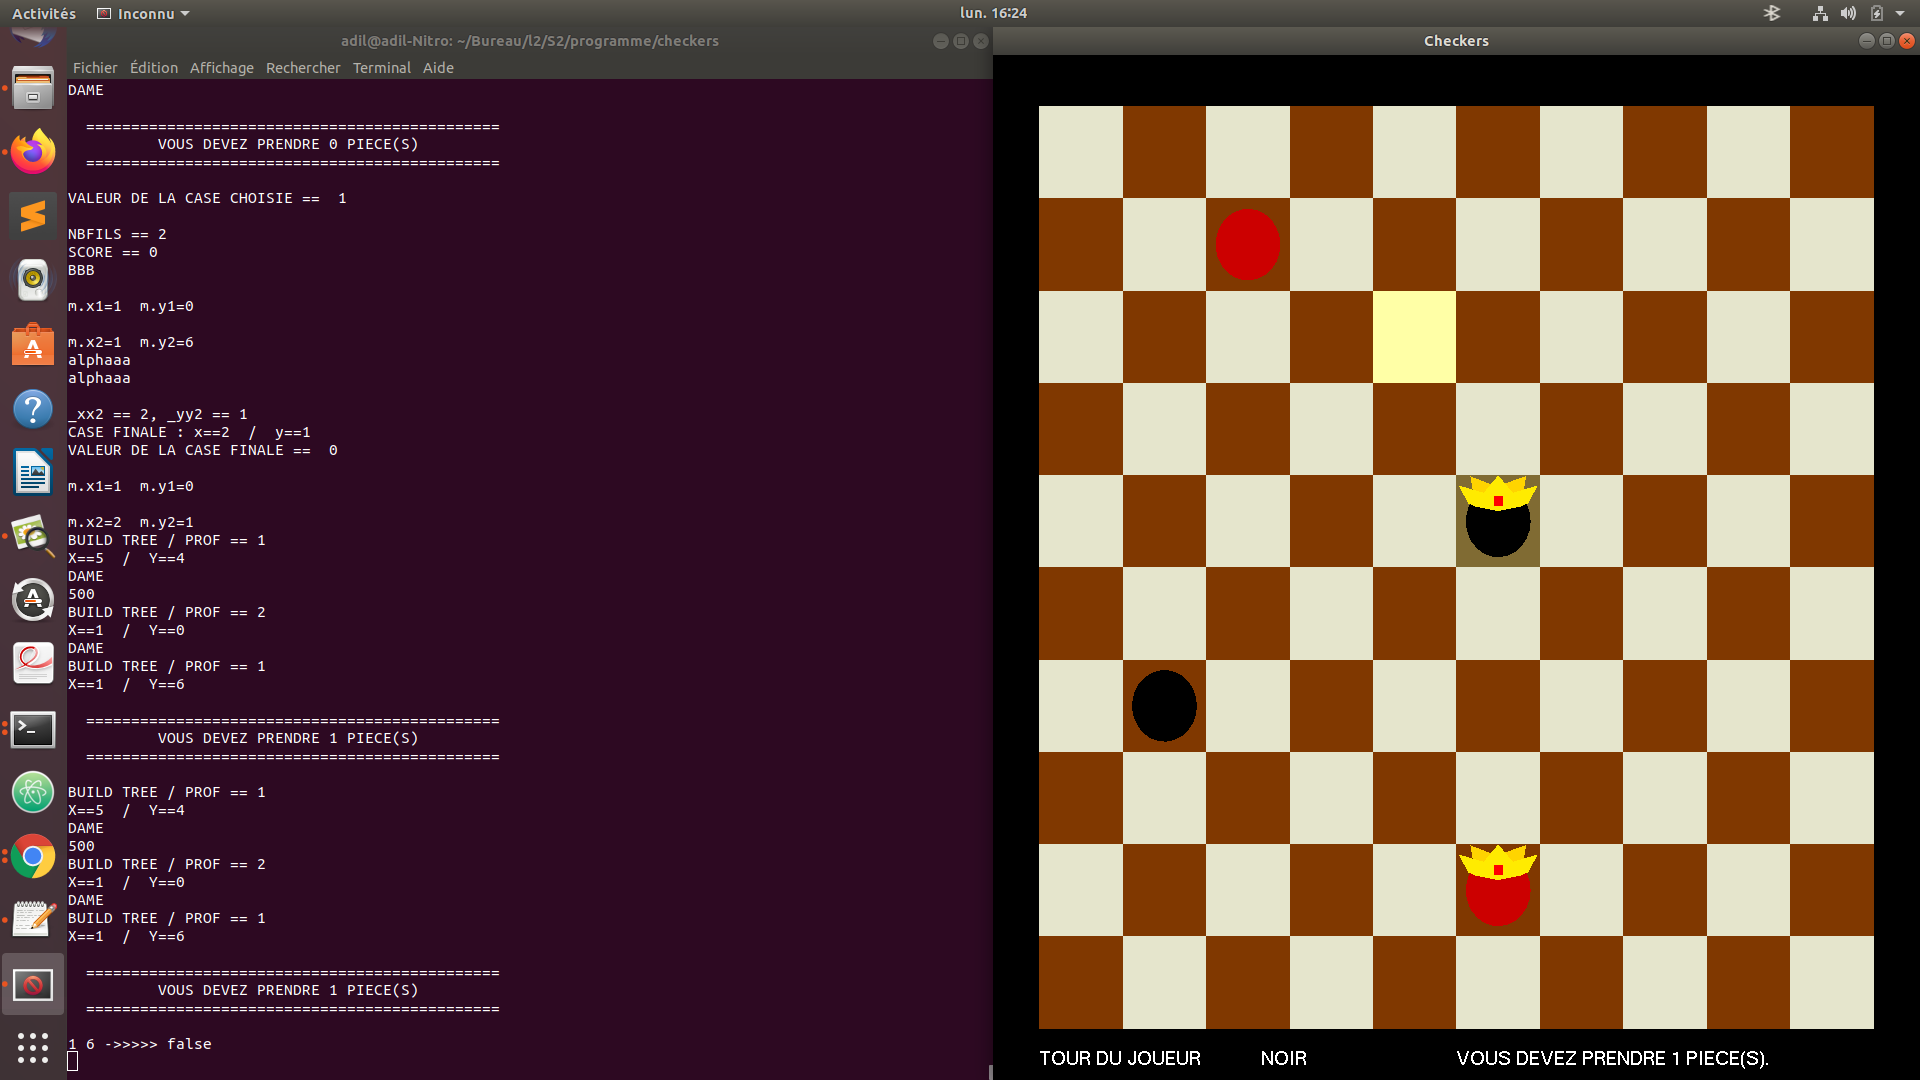
\includegraphics[width = 8cm, height = 5cm]{Reine.png}
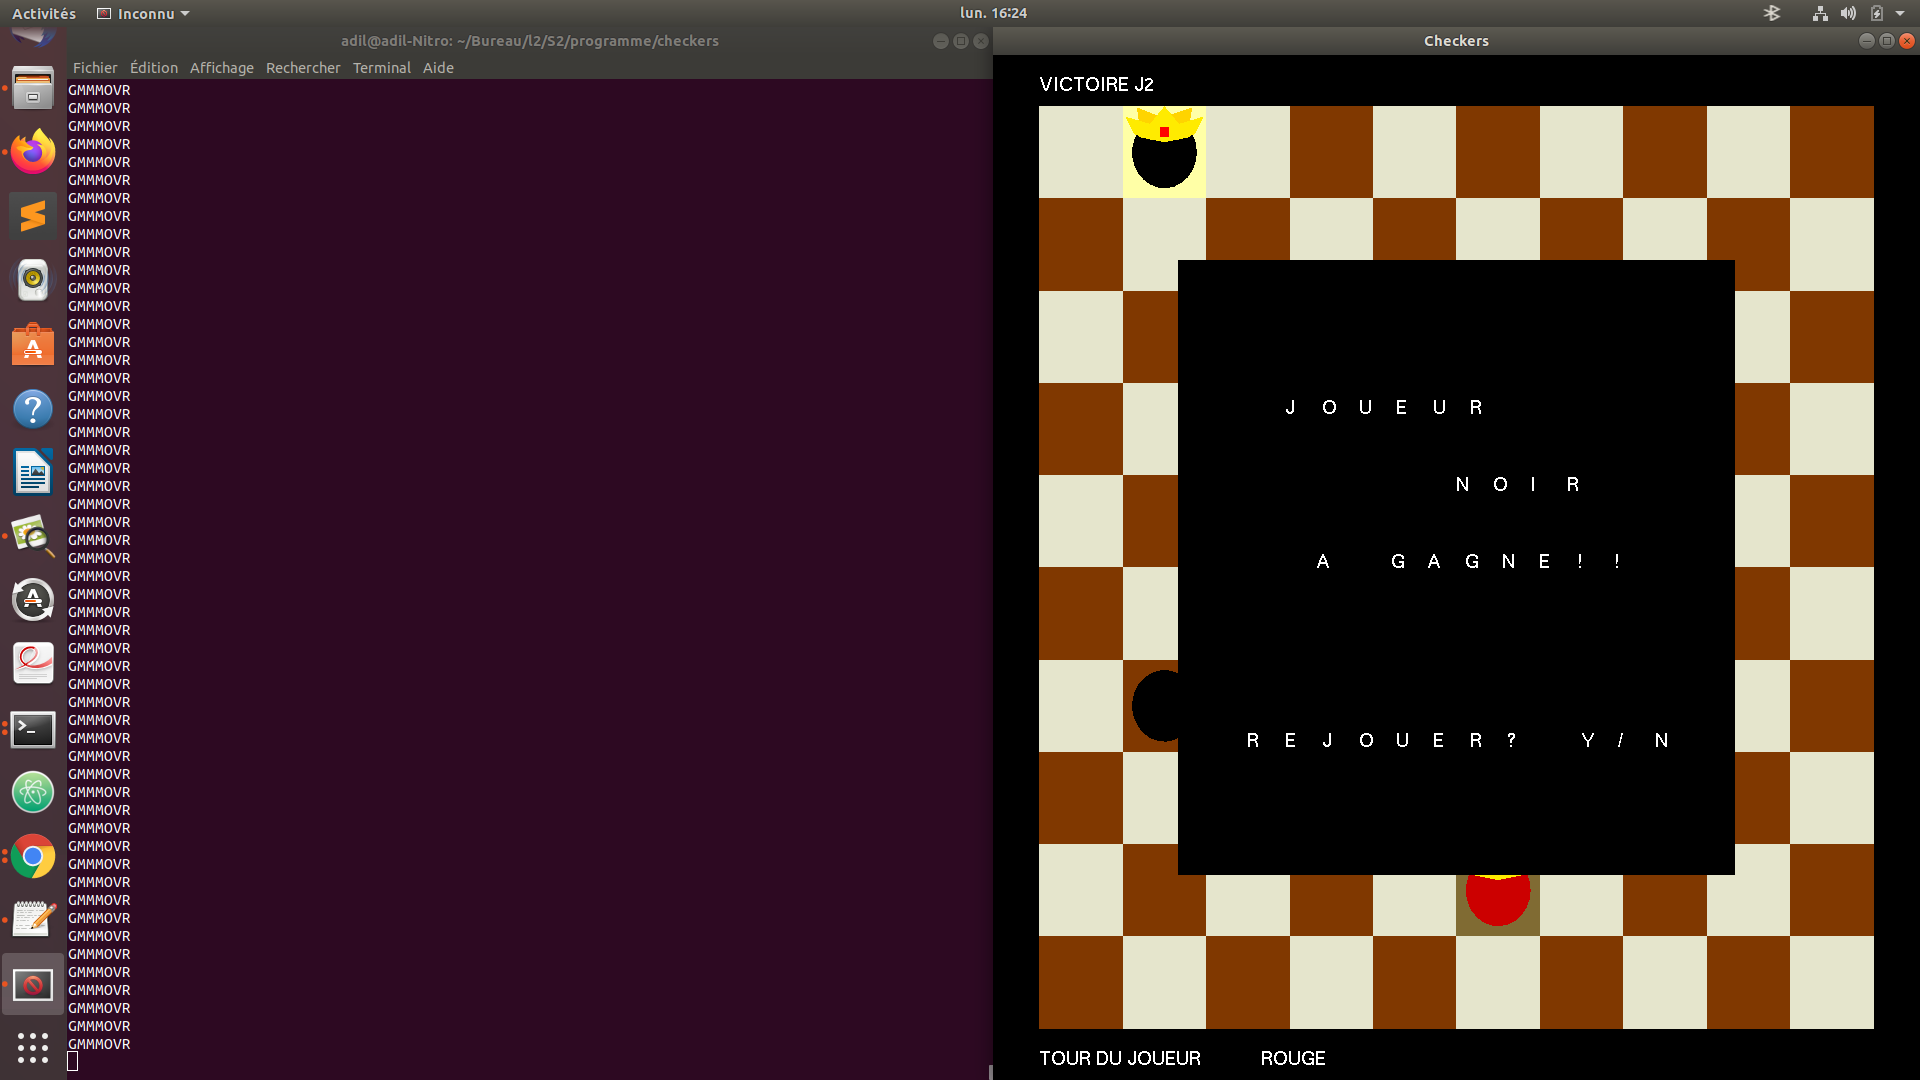
\includegraphics[width = 8cm, height = 5cm]{Reine2.png}
\bigbreak


\bigbreak
\bigbreak
\bigbreak
\bigbreak
\bigbreak
\bigbreak
\bigbreak
\bigbreak
\large\bf{Egalité : }
\bigbreak

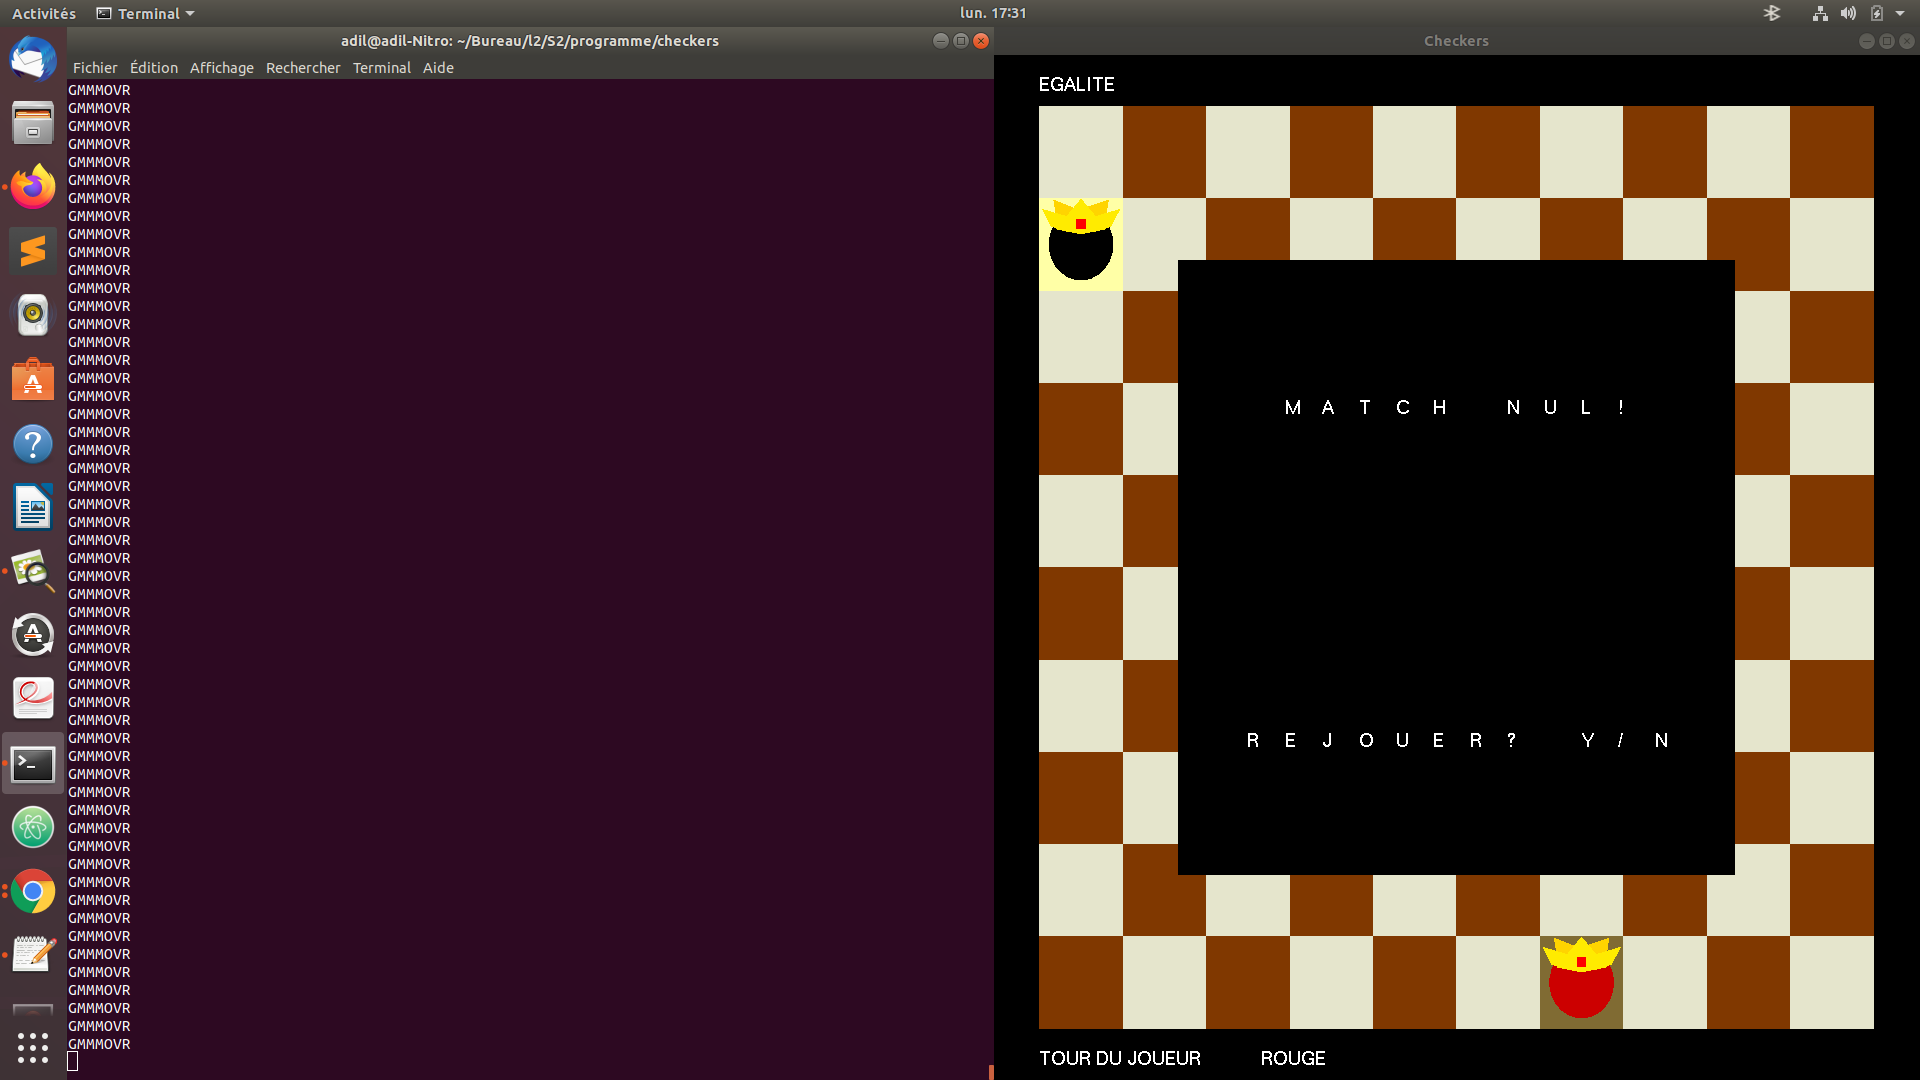
\includegraphics[width = 8cm, height = 5cm]{egalite.png}
\bigbreak



\large\bf{Hints : }
\bigbreak


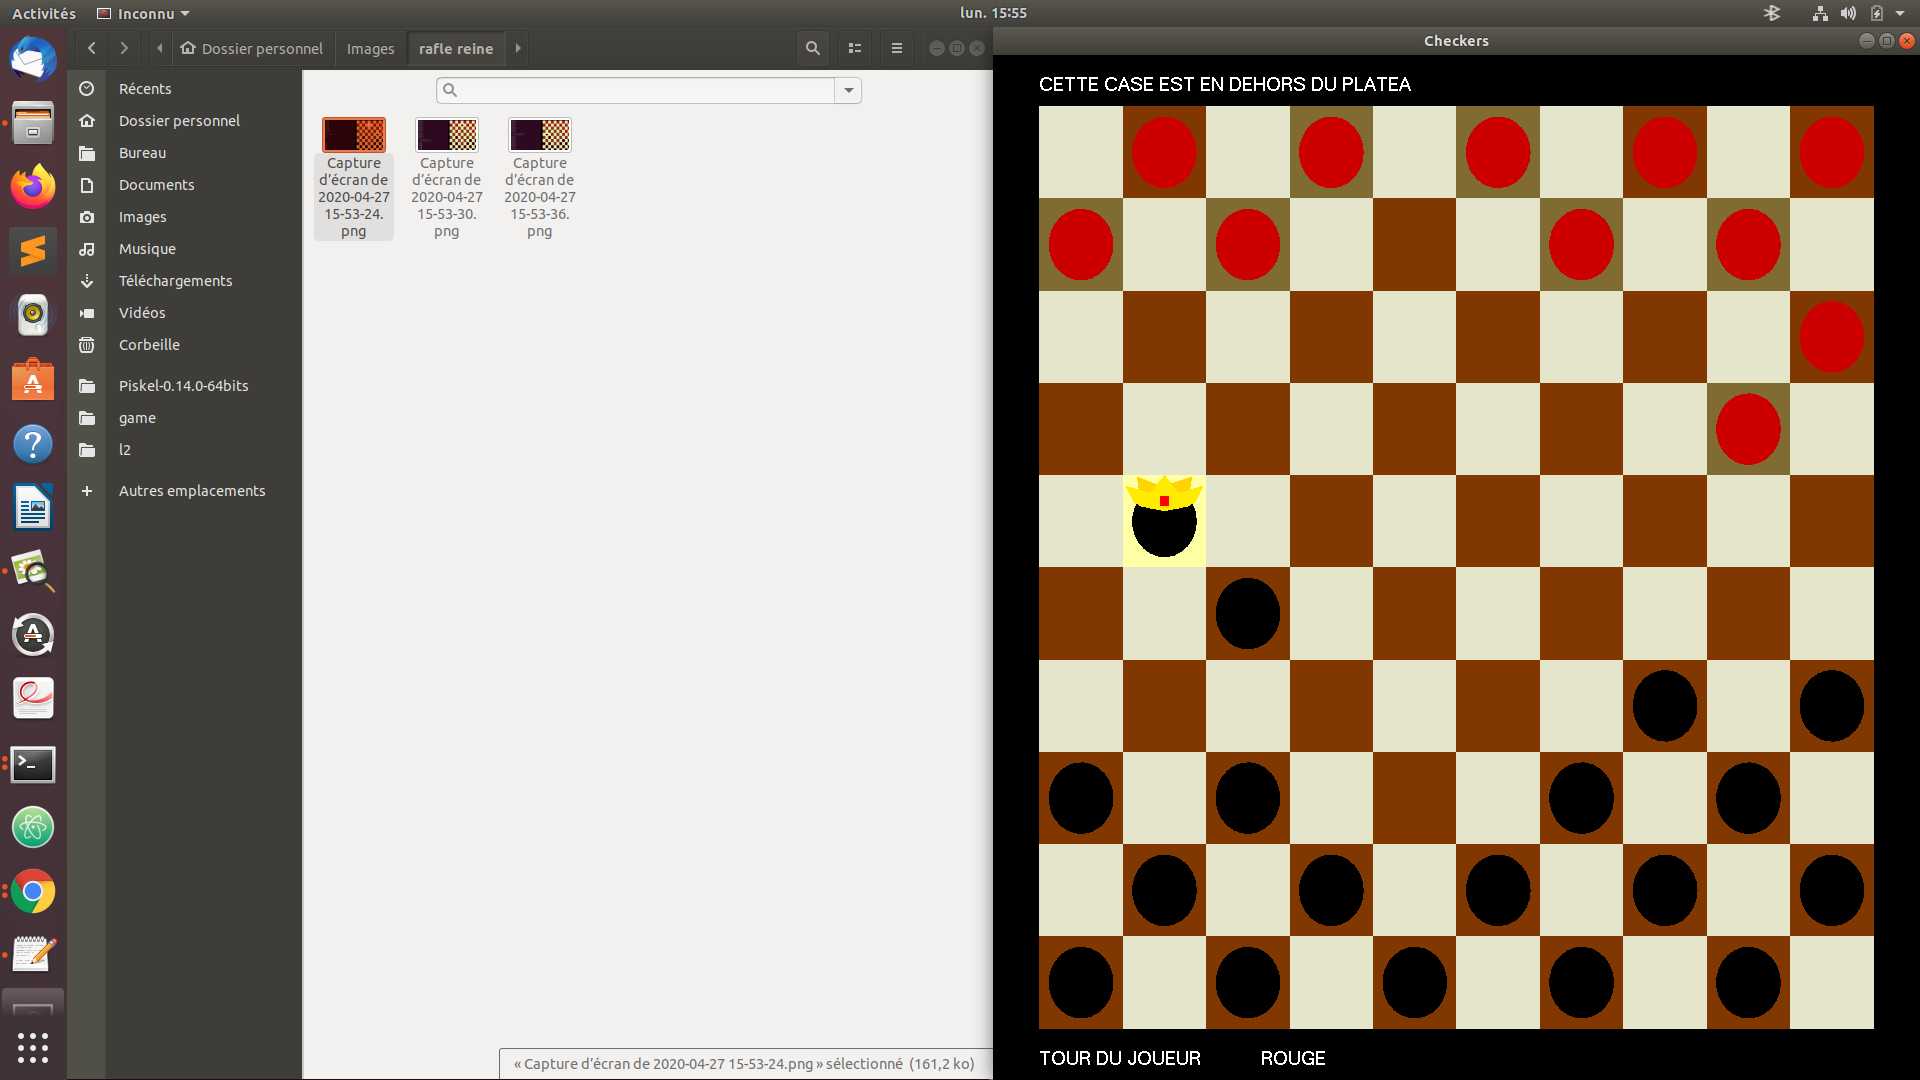
\includegraphics[width = 8cm, height = 5cm]{hints1.png}
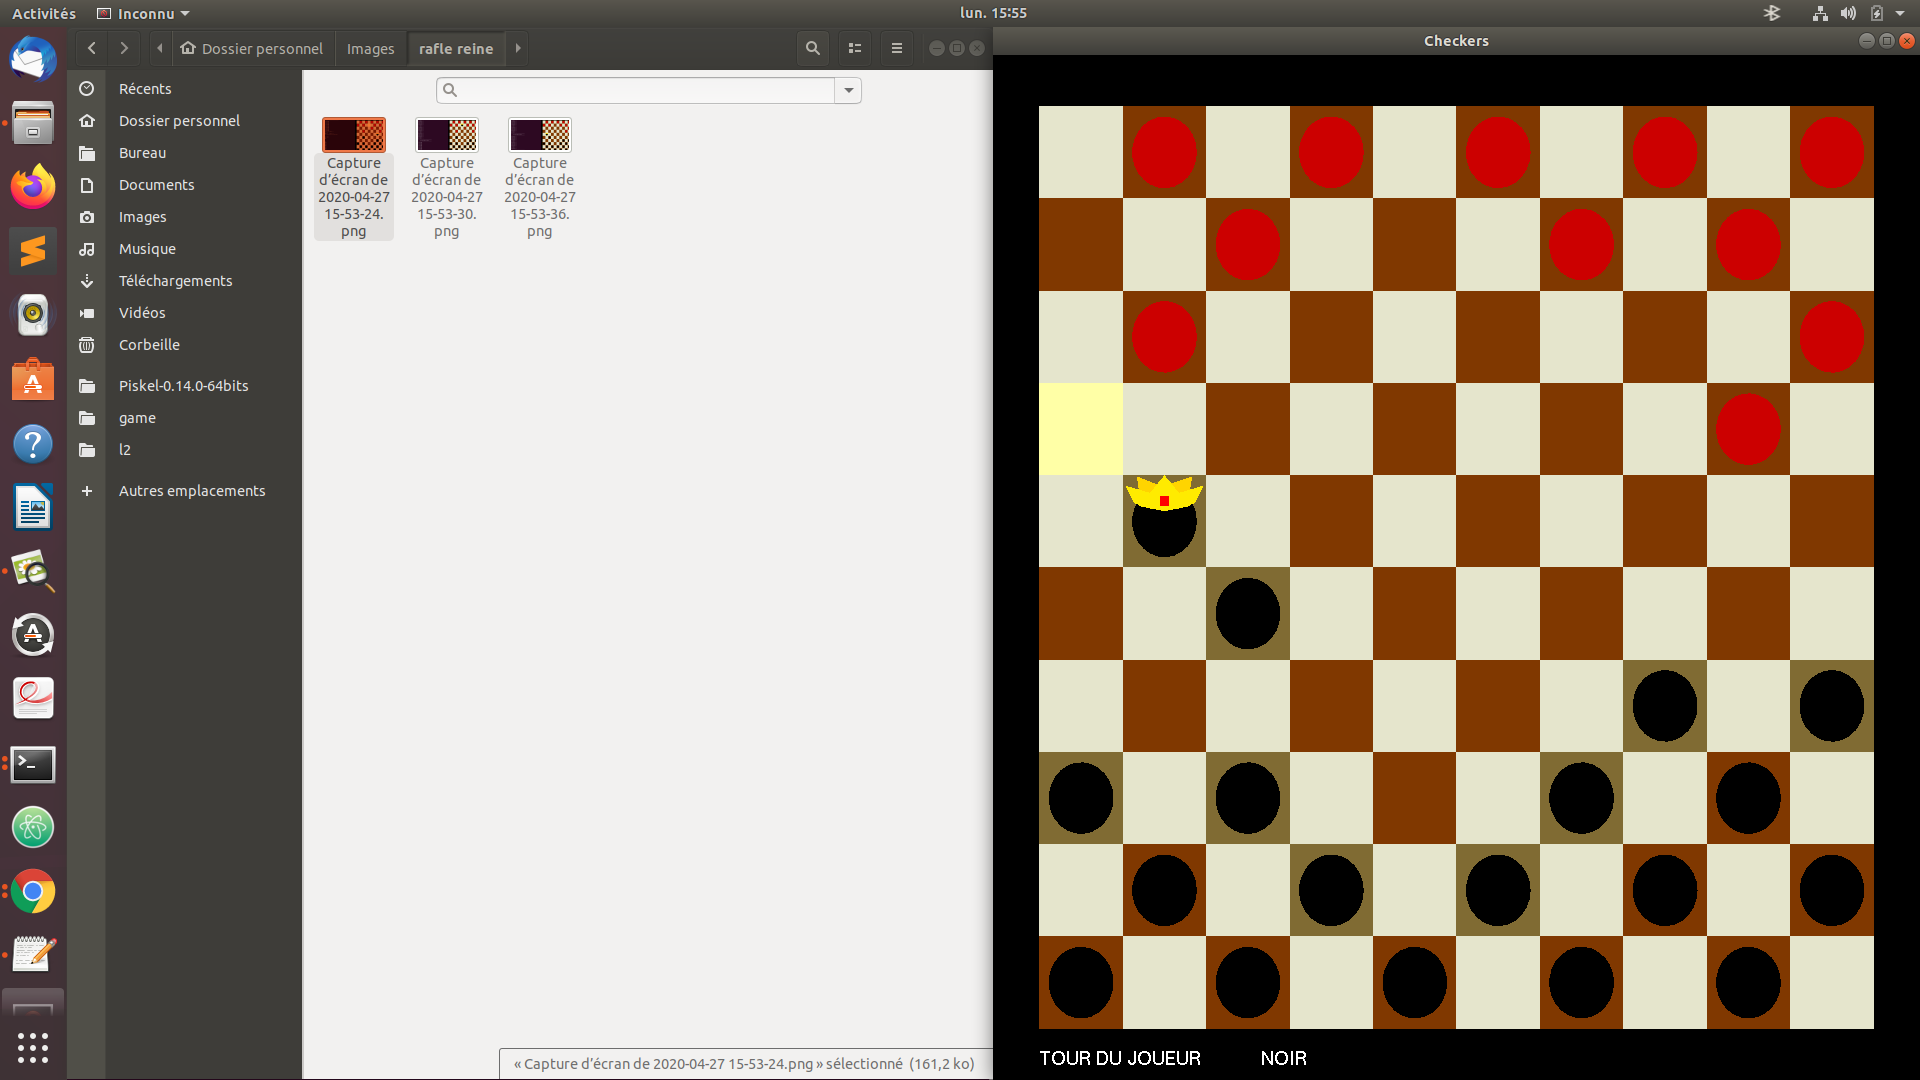
\includegraphics[width = 8cm, height = 5cm]{hints2.png}
\bigbreak
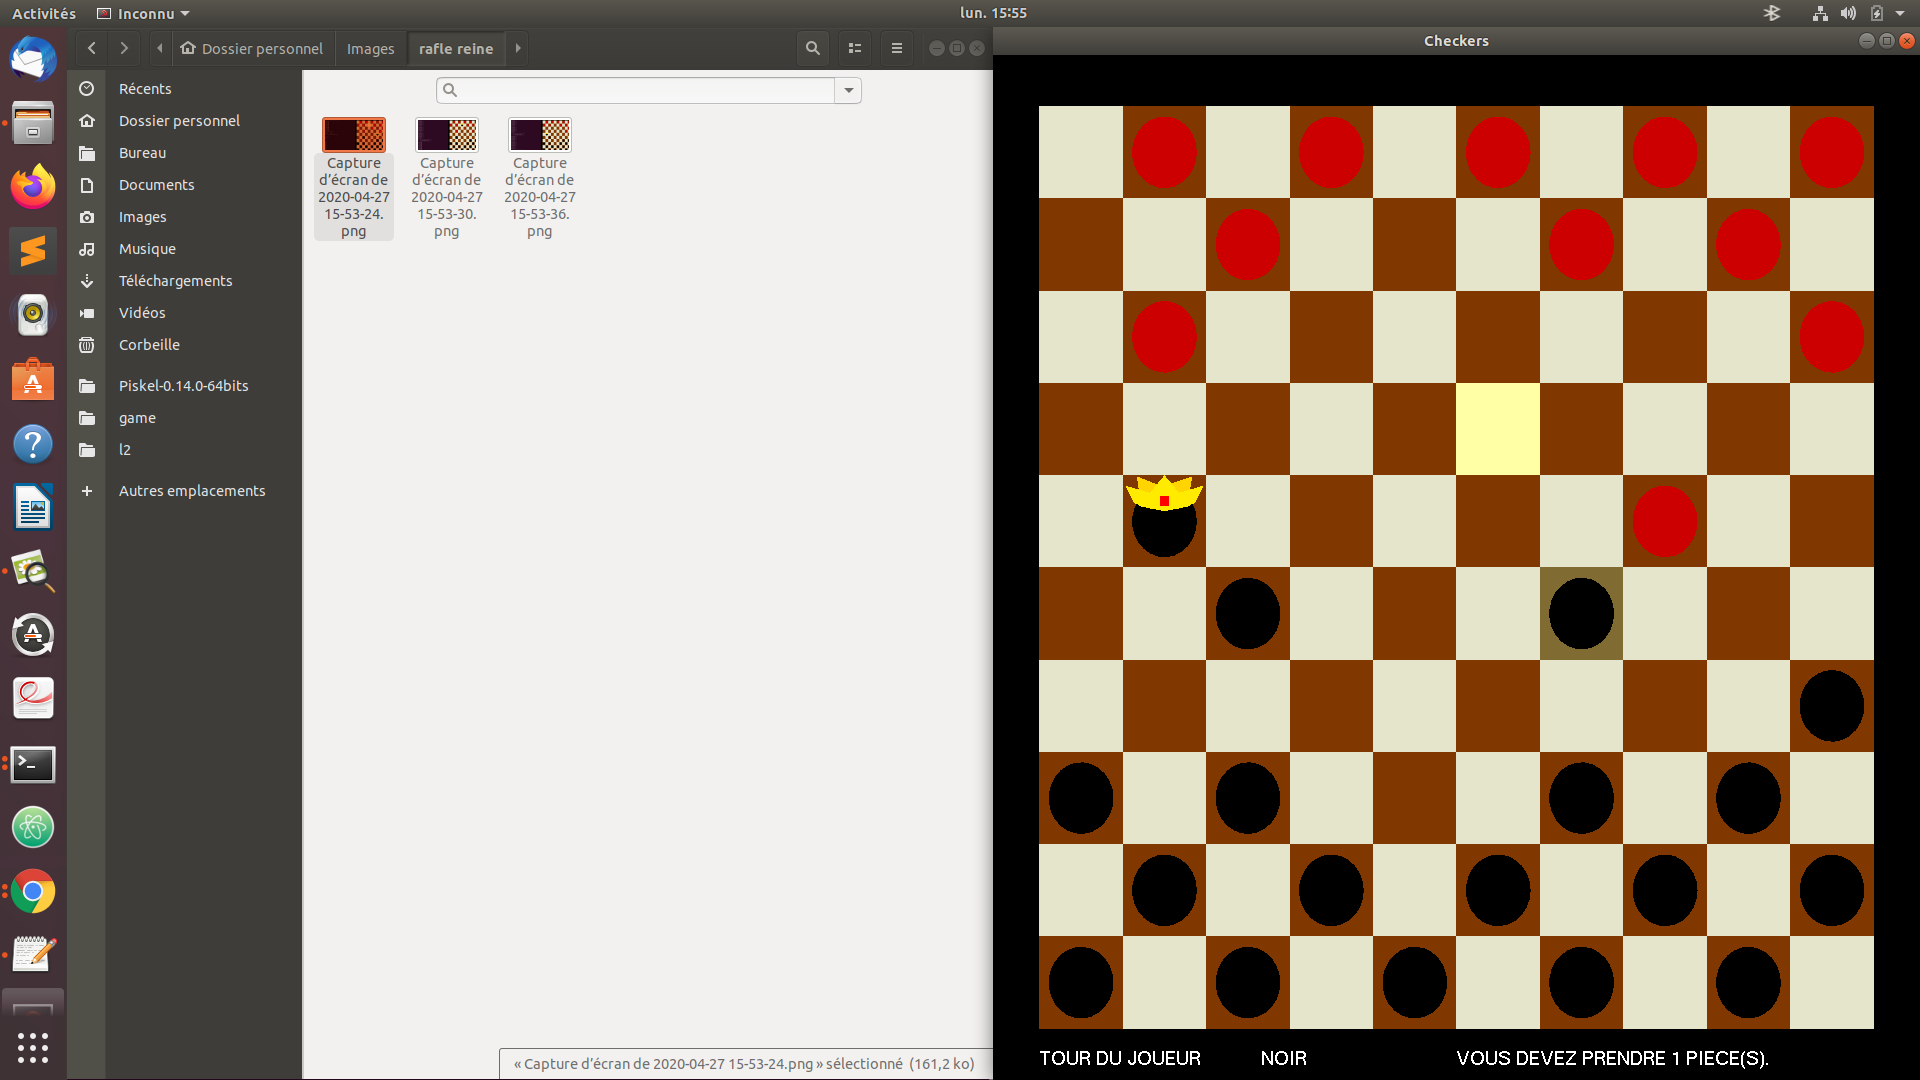
\includegraphics[width = 8cm, height = 5cm]{hints3.png}
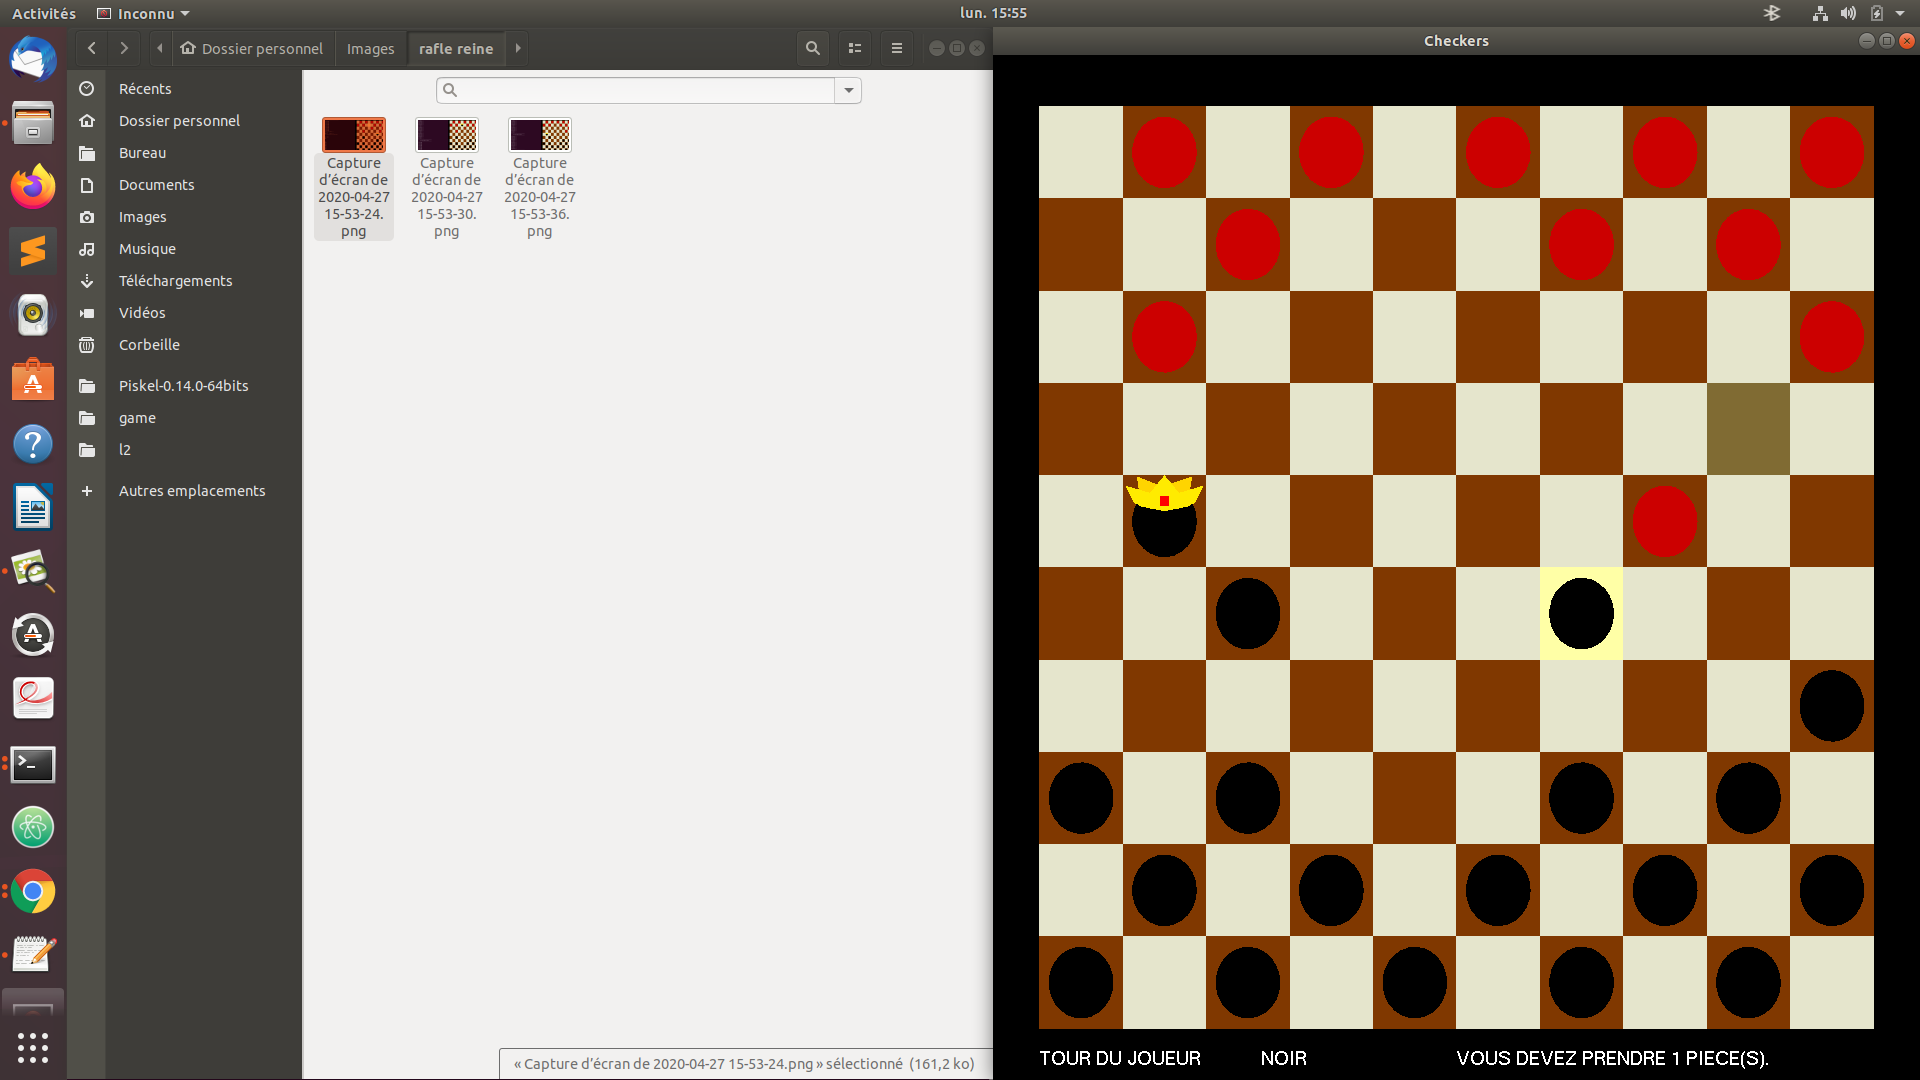
\includegraphics[width = 8cm, height = 5cm]{hints4.png}


\bigbreak
\large\bf{Rafle double : }
\bigbreak



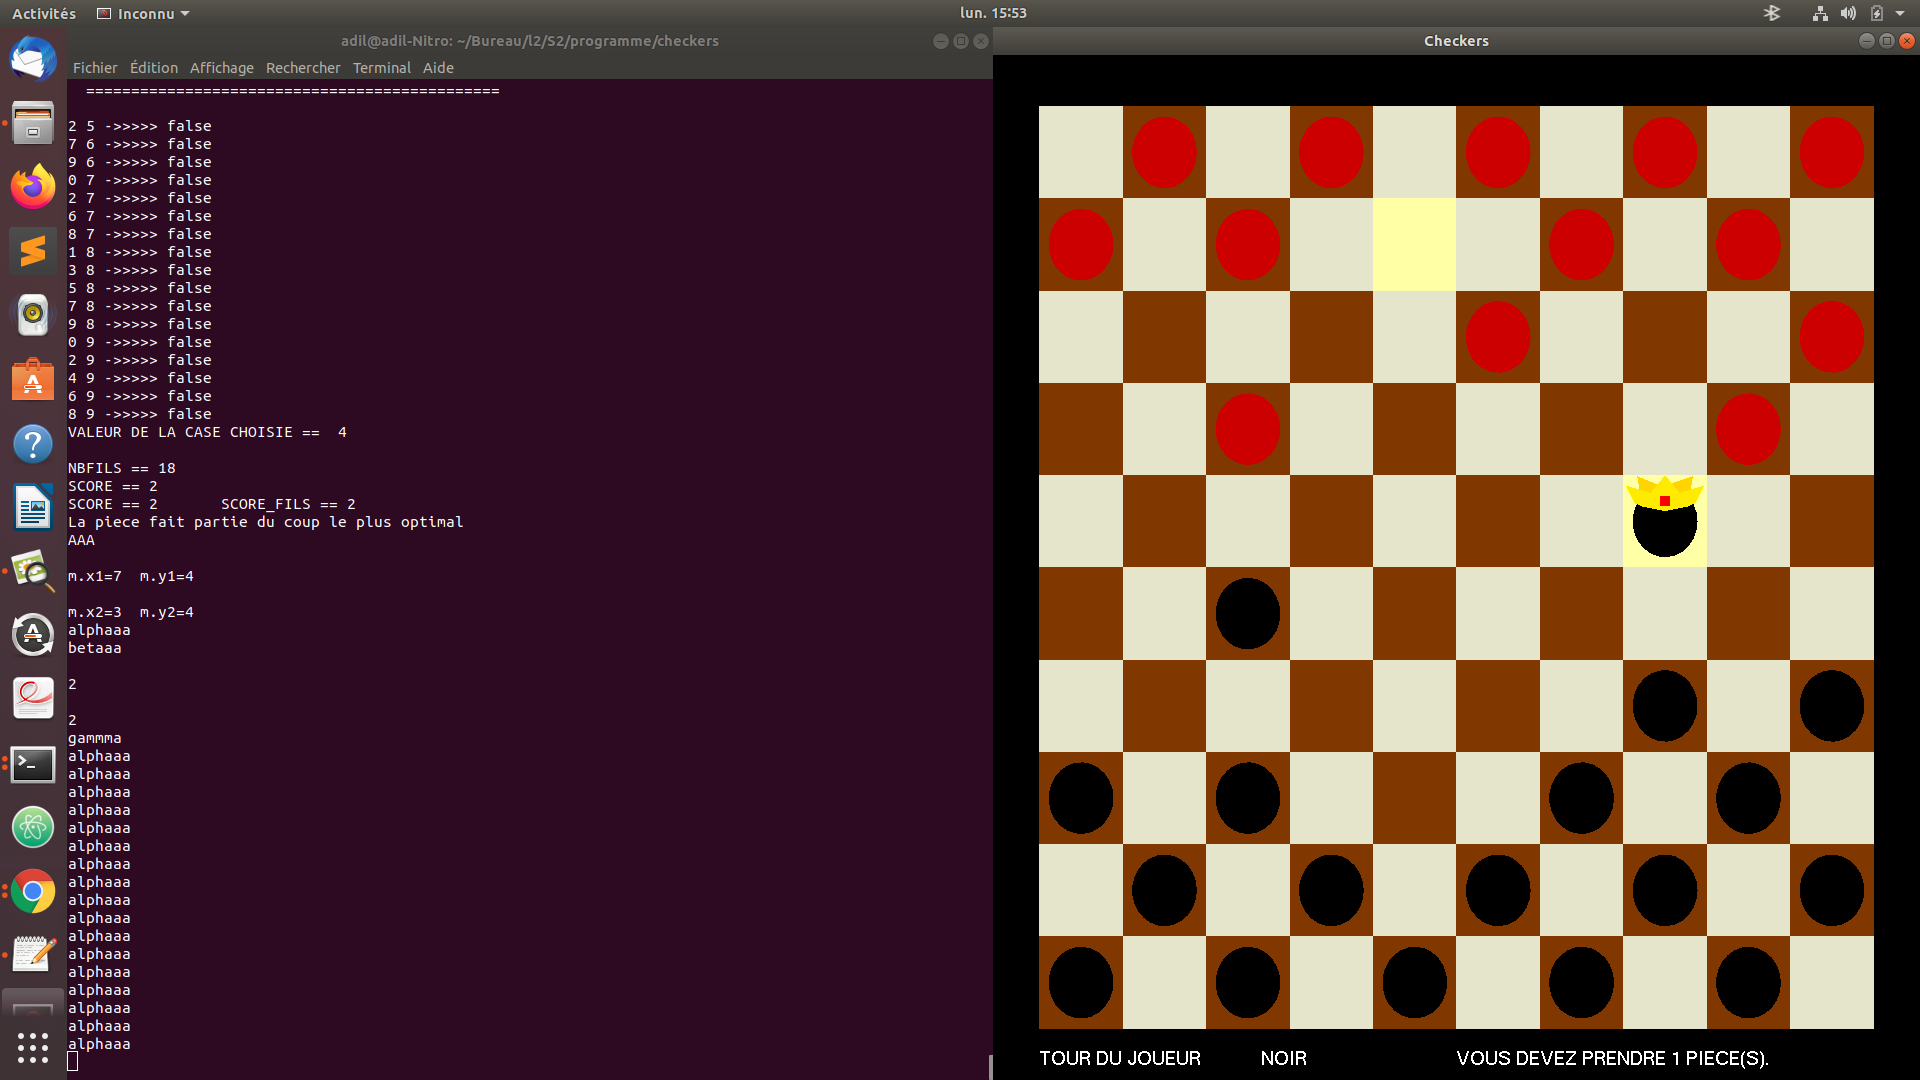
\includegraphics[width = 8cm, height = 5cm]{rafle2-1.png}
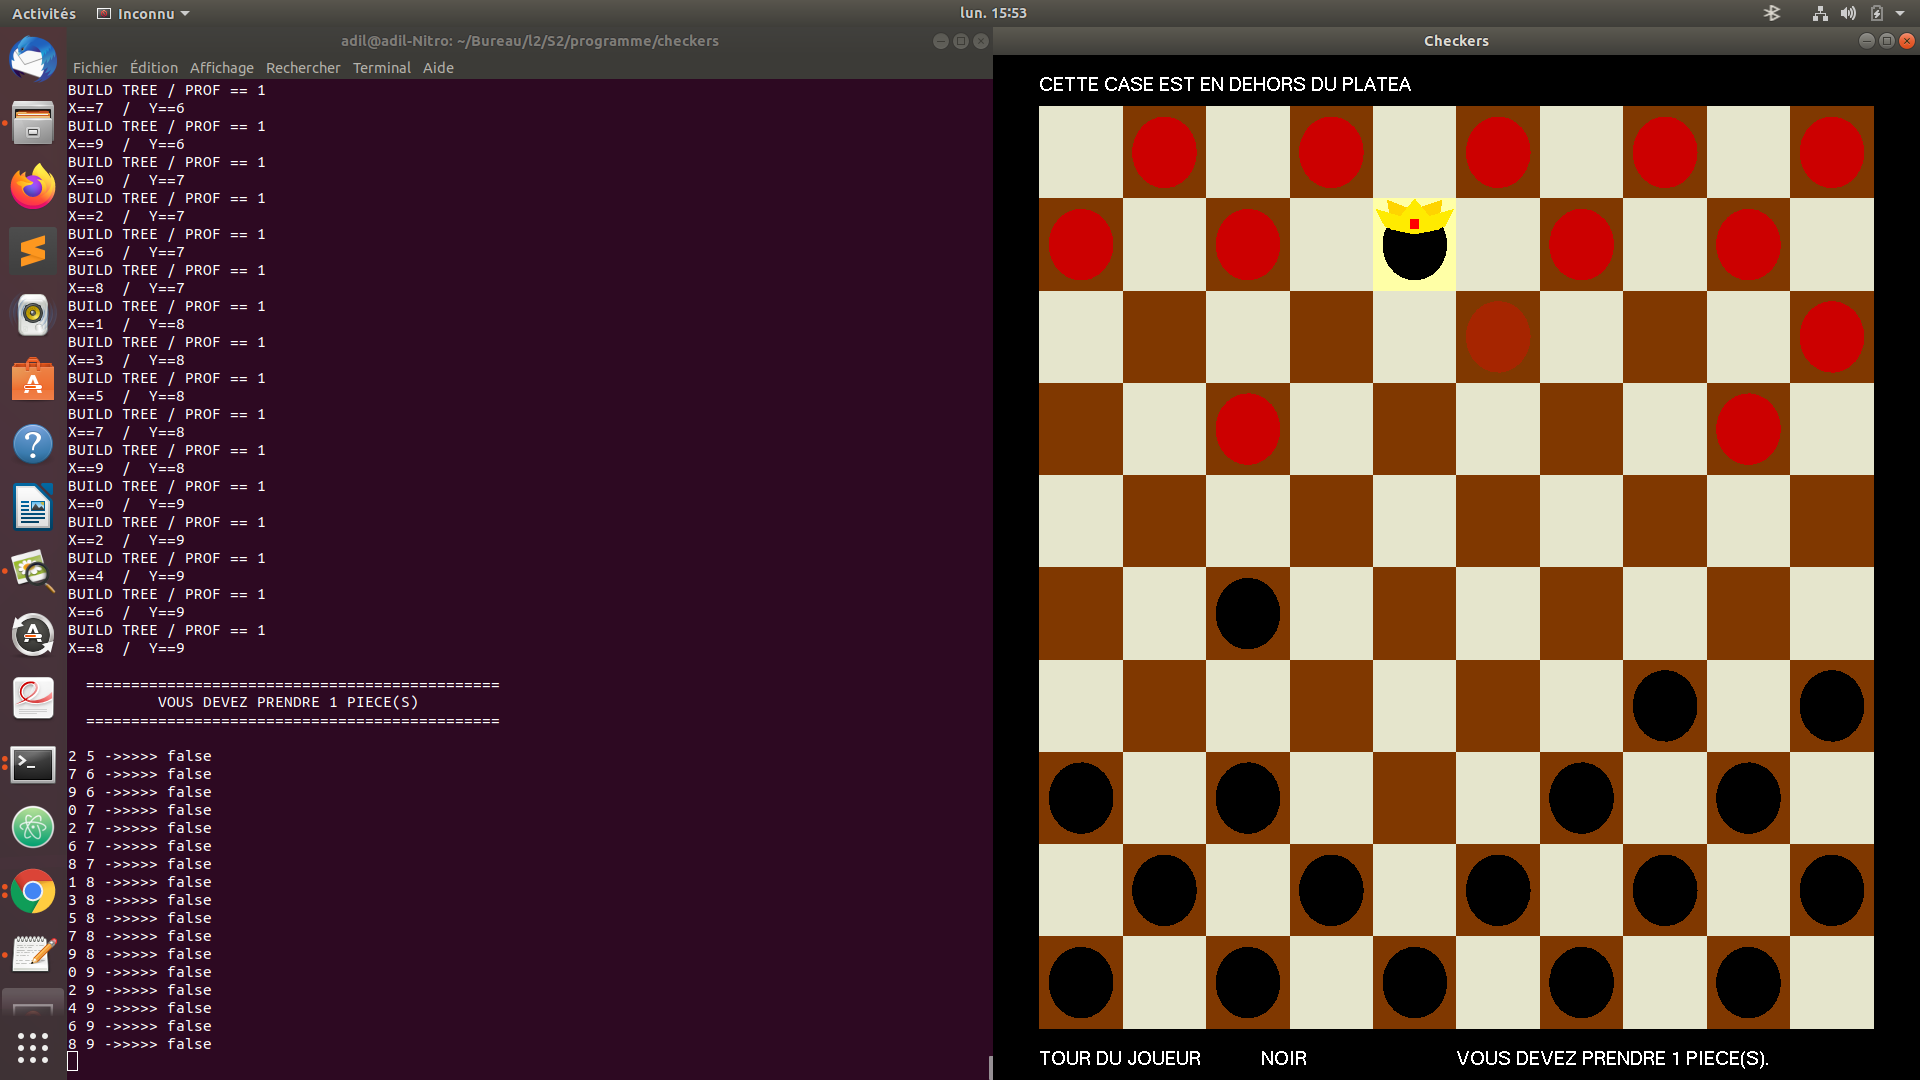
\includegraphics[width = 8cm, height = 5cm]{rafle2-2.png}
\bigbreak
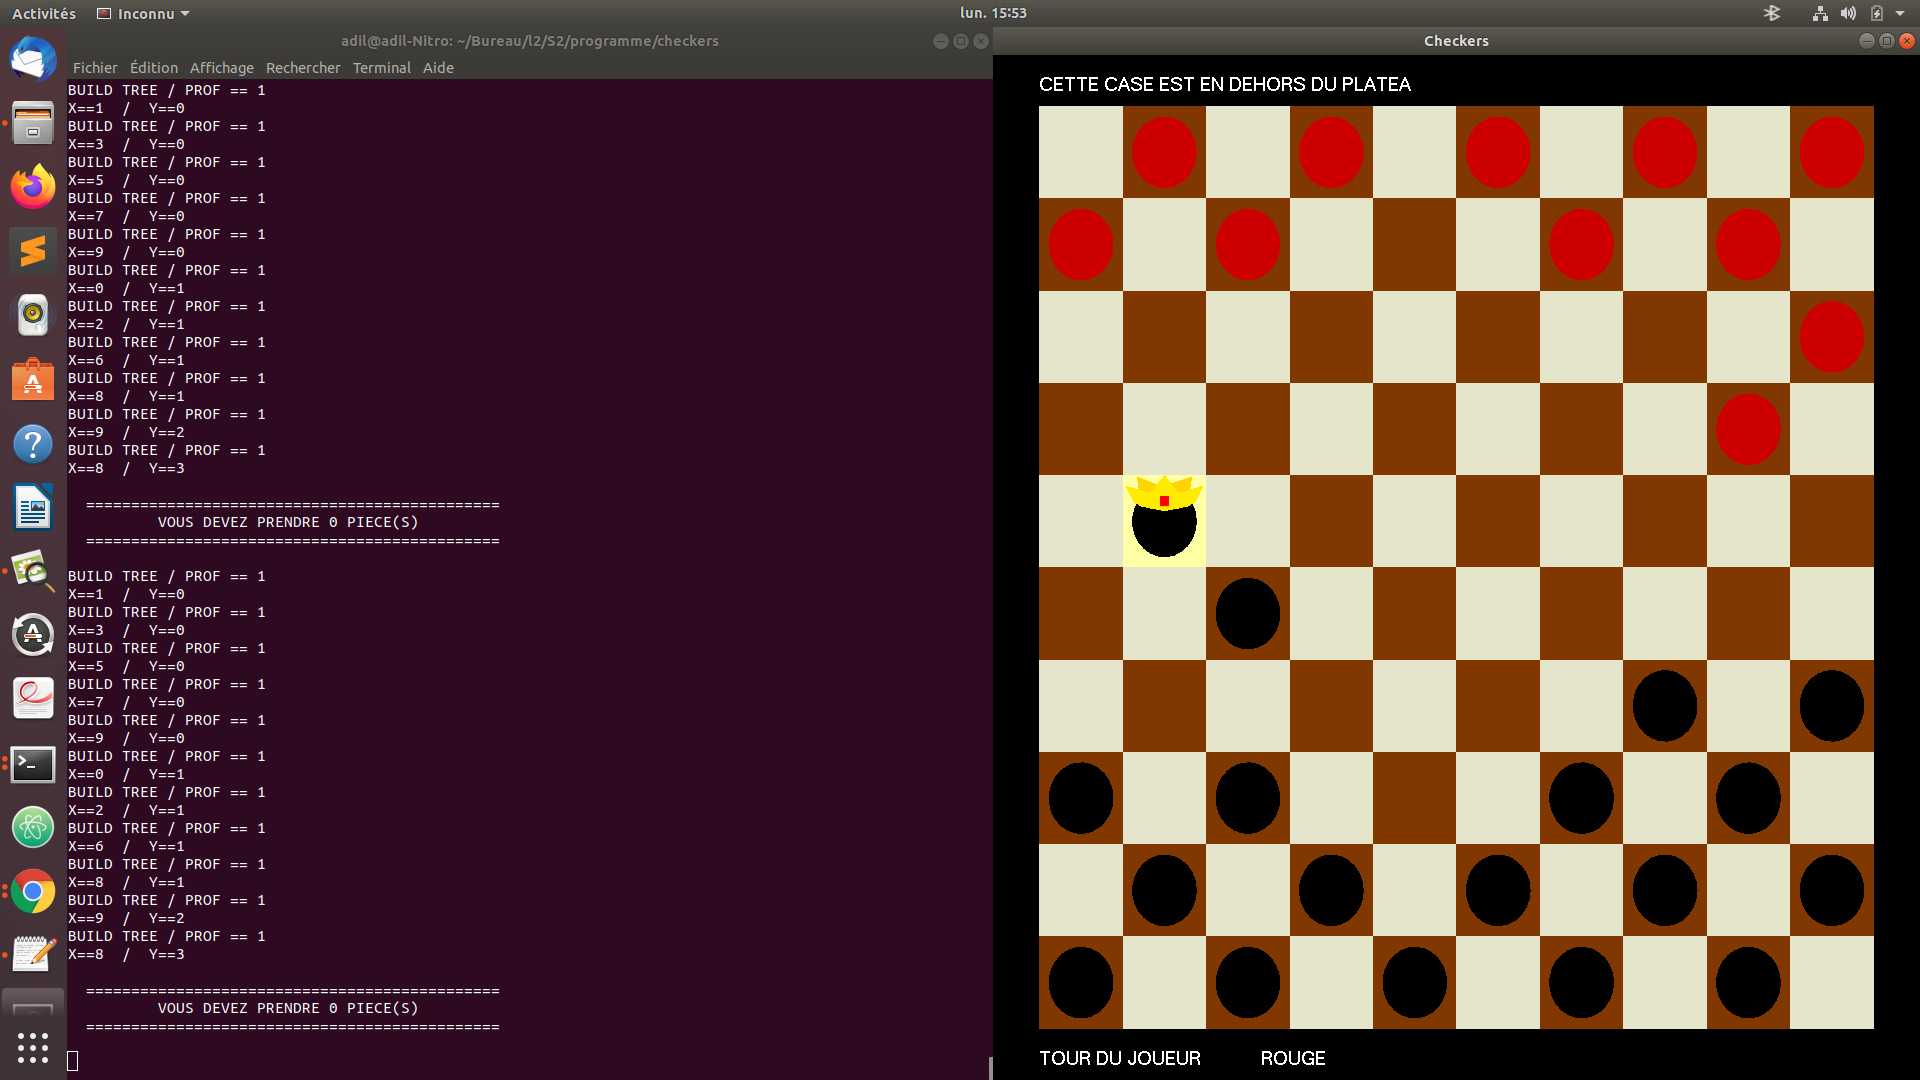
\includegraphics[width = 8cm, height = 5cm]{rafle2-3.png}



\bigbreak
\large\bf{Rafle triple : }
\bigbreak


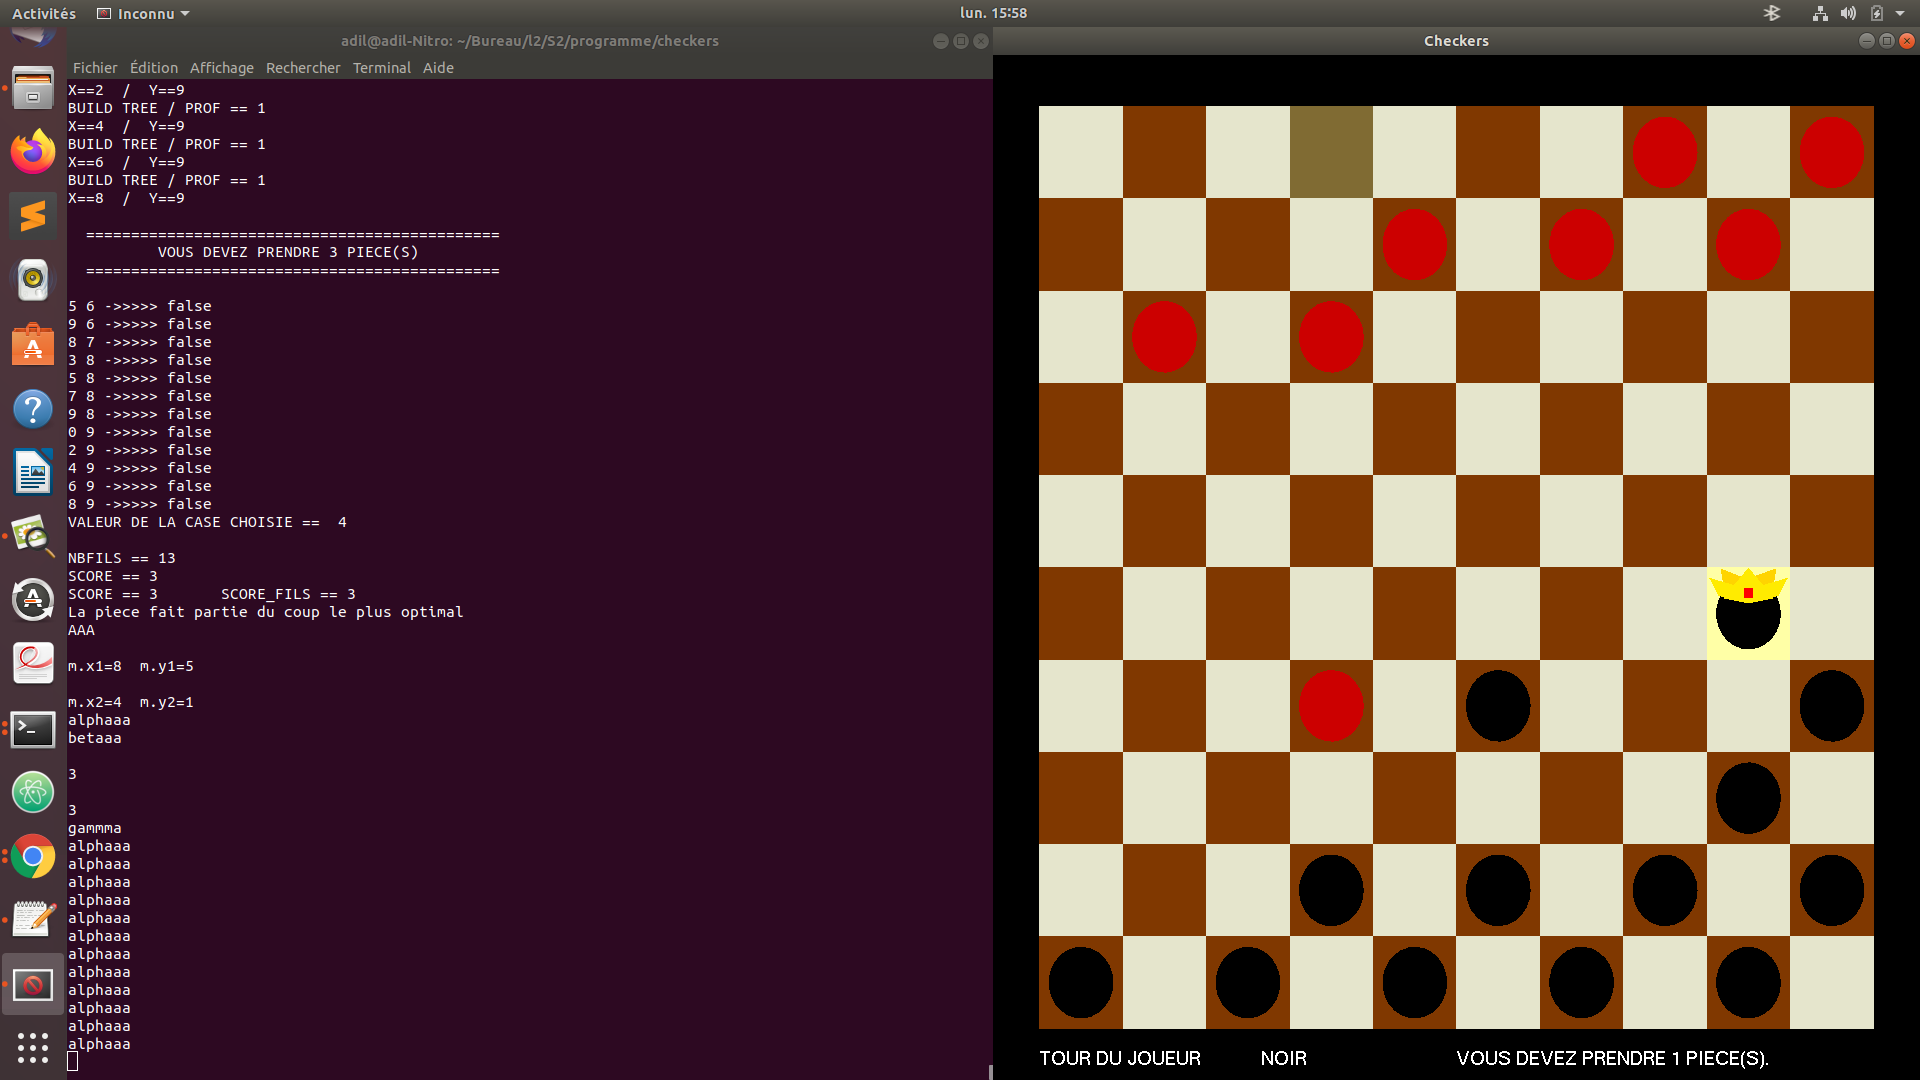
\includegraphics[width = 8cm, height = 5cm]{rafle3-1.png}
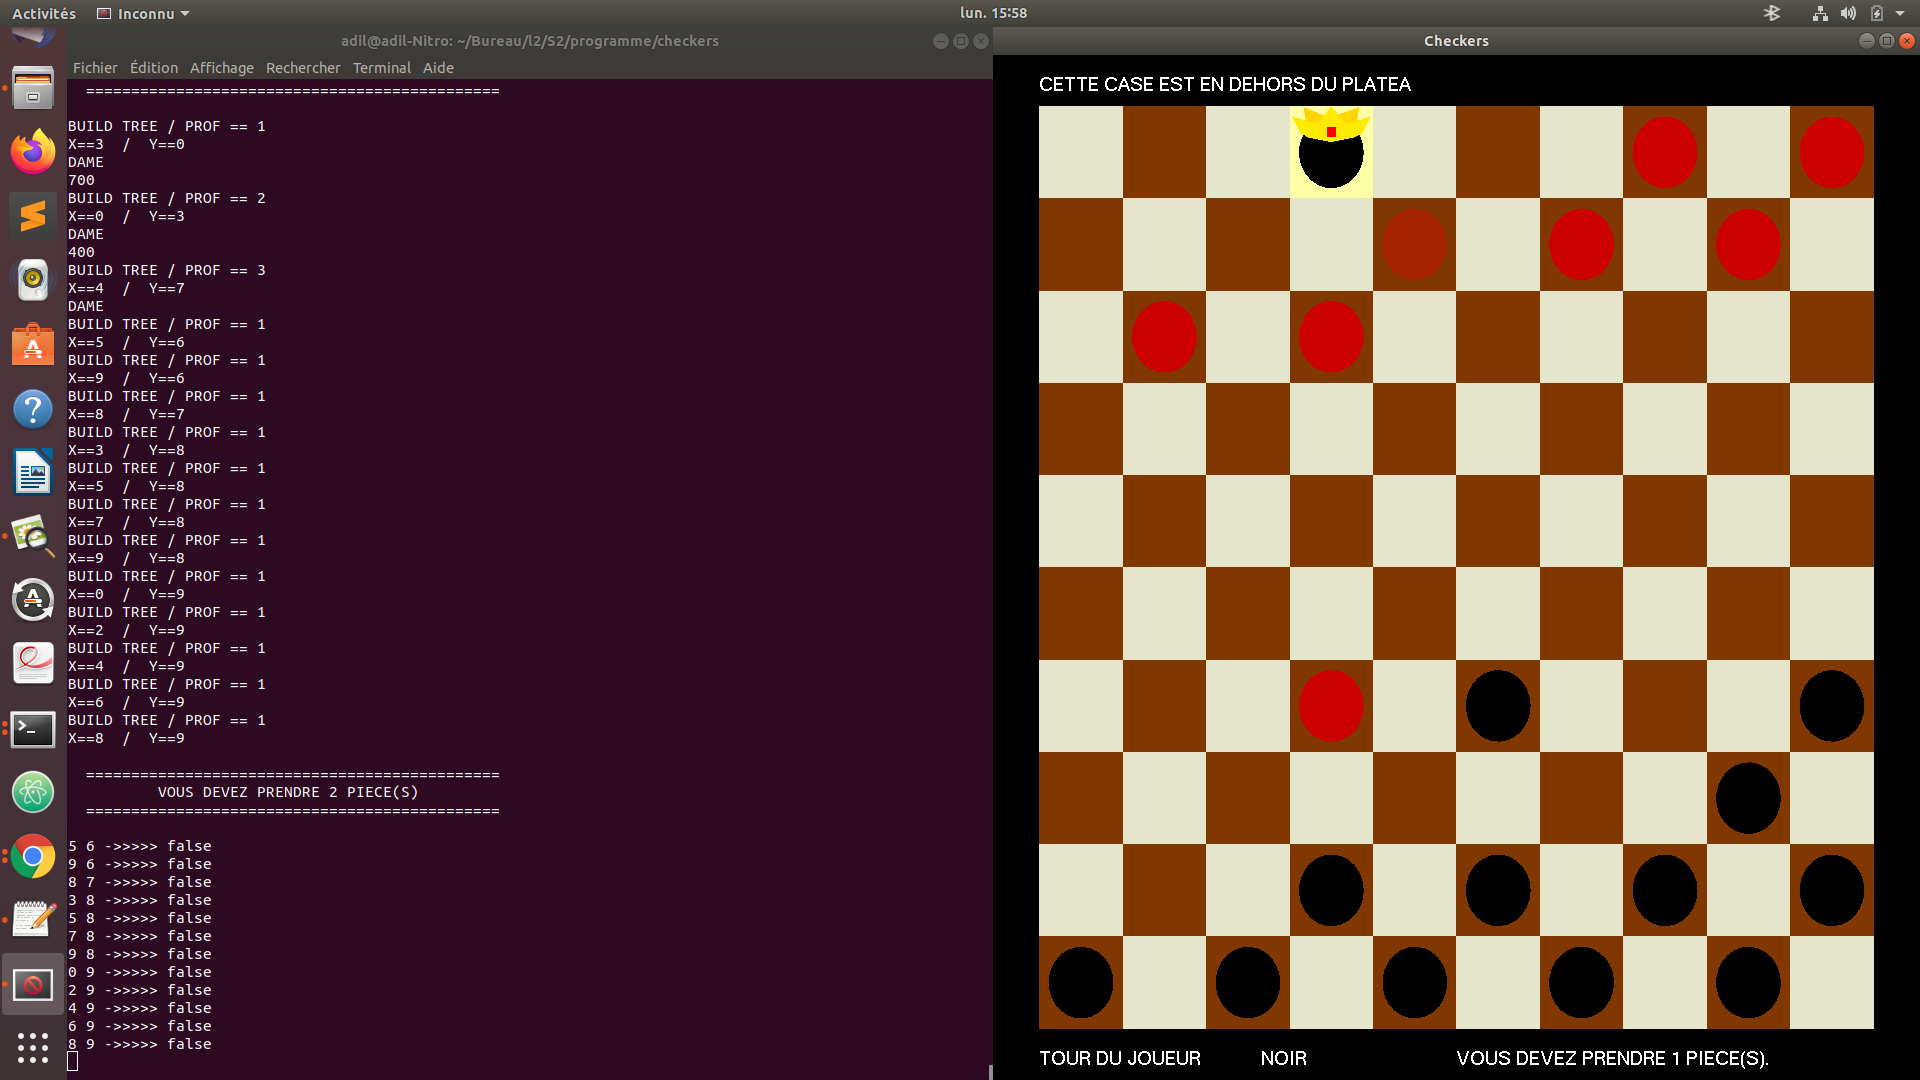
\includegraphics[width = 8cm, height = 5cm]{rafle3-2.png}
\bigbreak
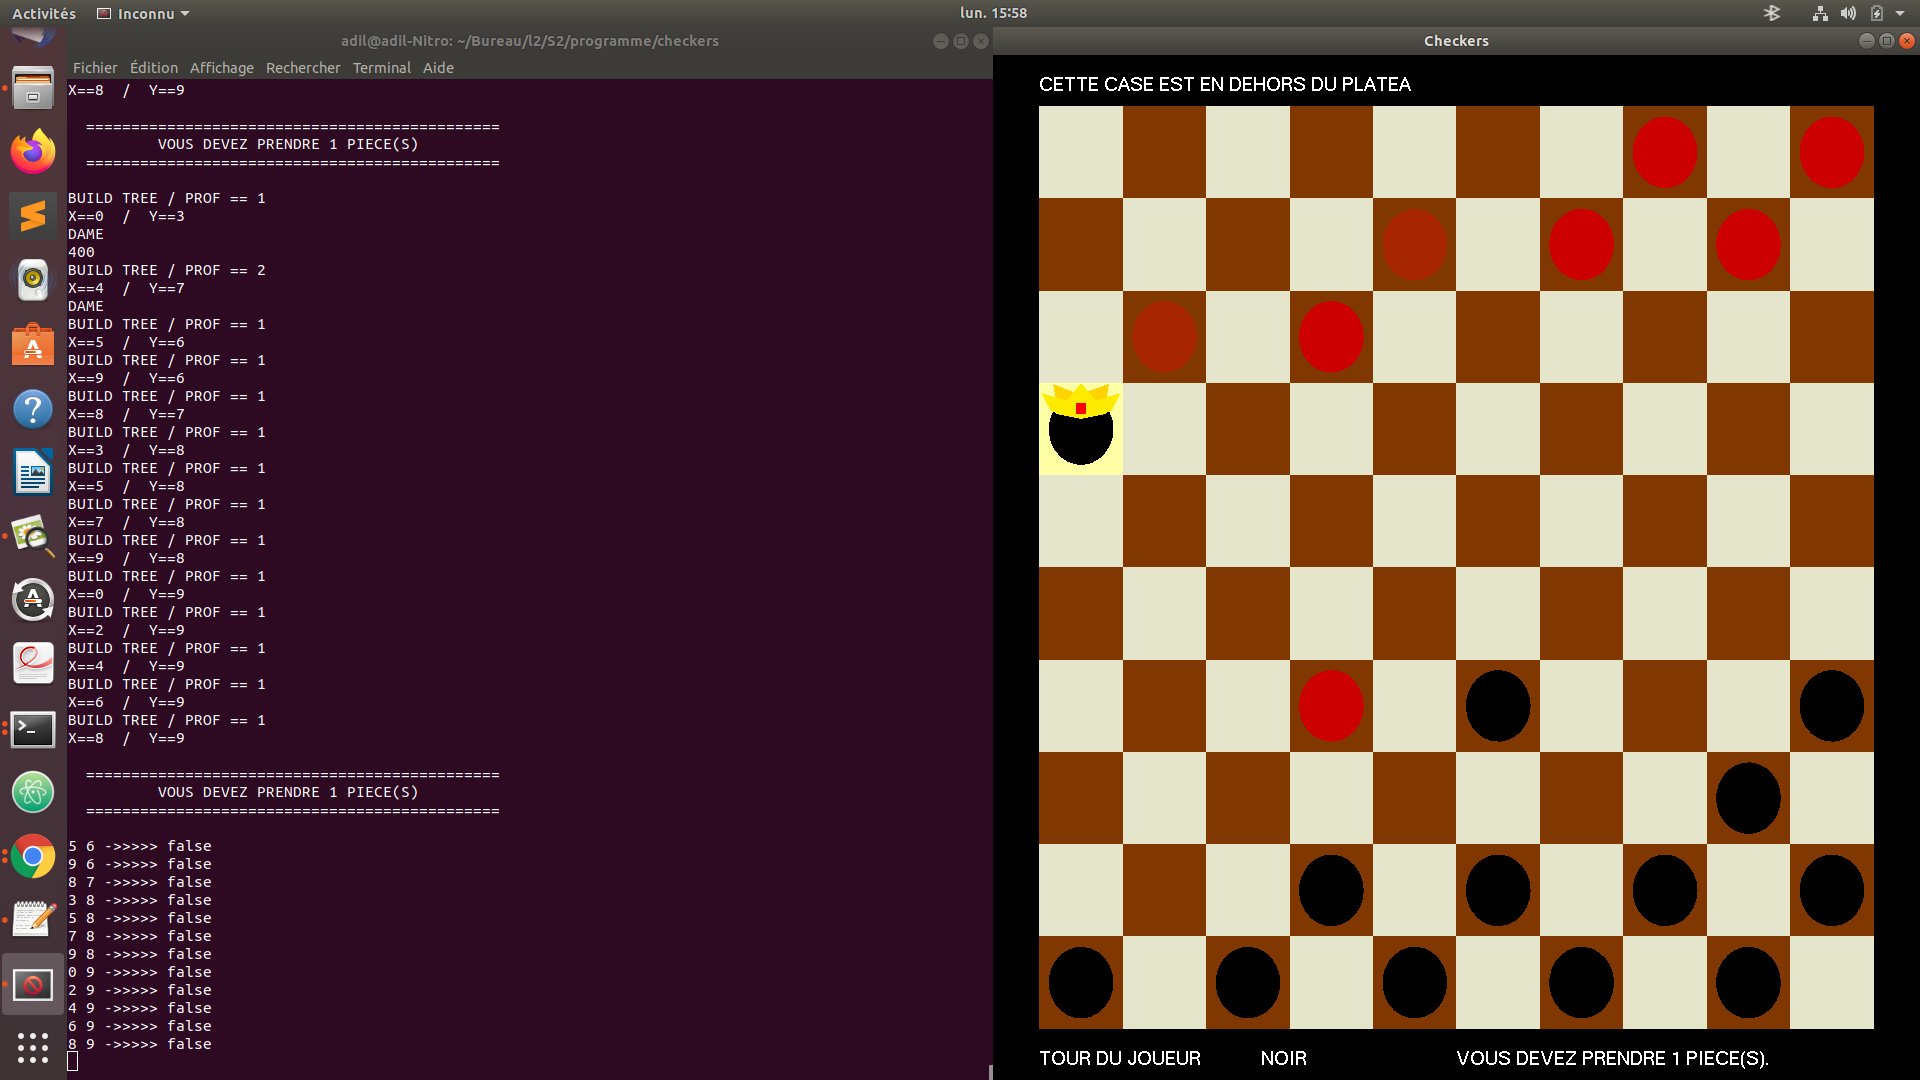
\includegraphics[width = 8cm, height = 5cm]{rafle3-3.png}
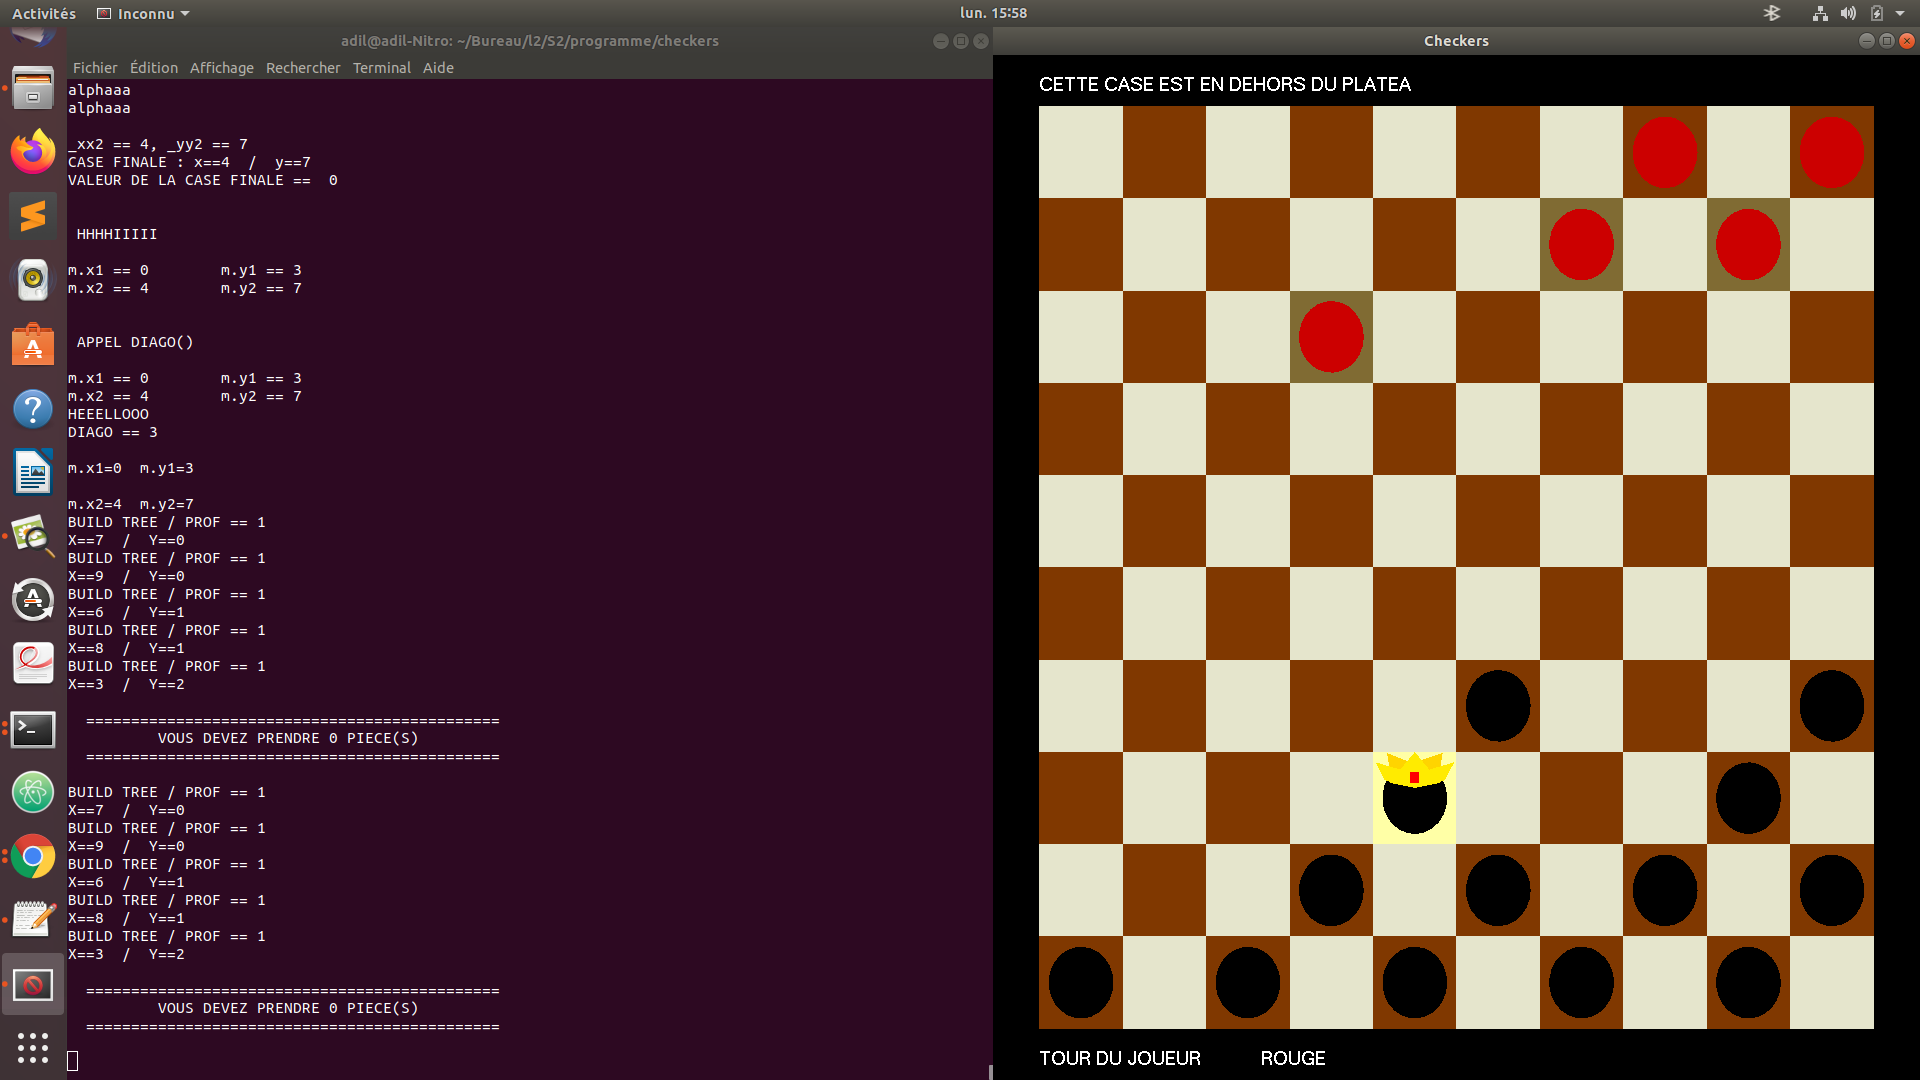
\includegraphics[width = 8cm, height = 5cm]{rafle3-4.png}

\section{Programme de tests}

\begin{verbatim}

Les tests effectués fonctionnent tous sans exception. Cette trace d'éxécution est 
seulement présente pour montrer que si echec il y a, le programme recence toutes les 
erreurs, leur nombre et indique sur quelle fonctionnalités elles ont lieu.

\end{verbatim}

\bigbreak
\large\bf {Test echoues :}
\bigbreak

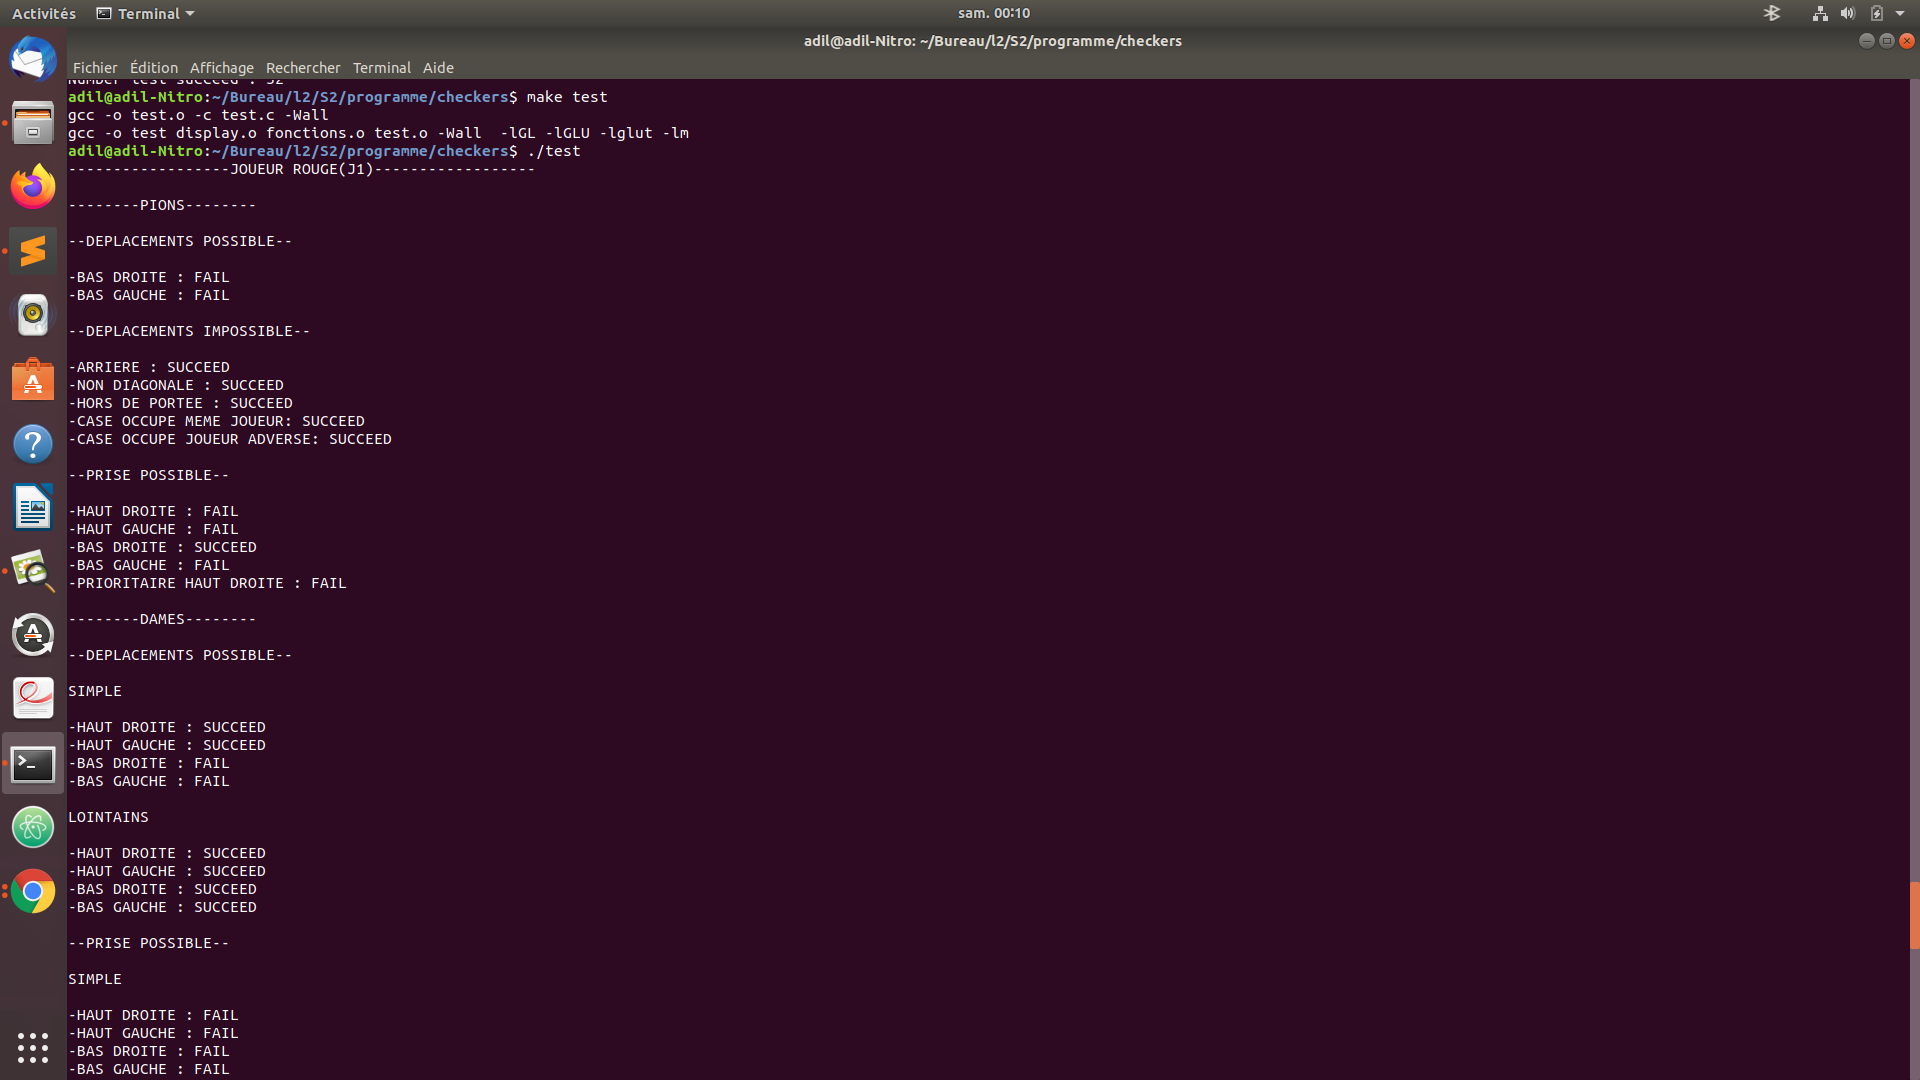
\includegraphics[width = 8cm, height = 5cm]{TestEchoue1.png}
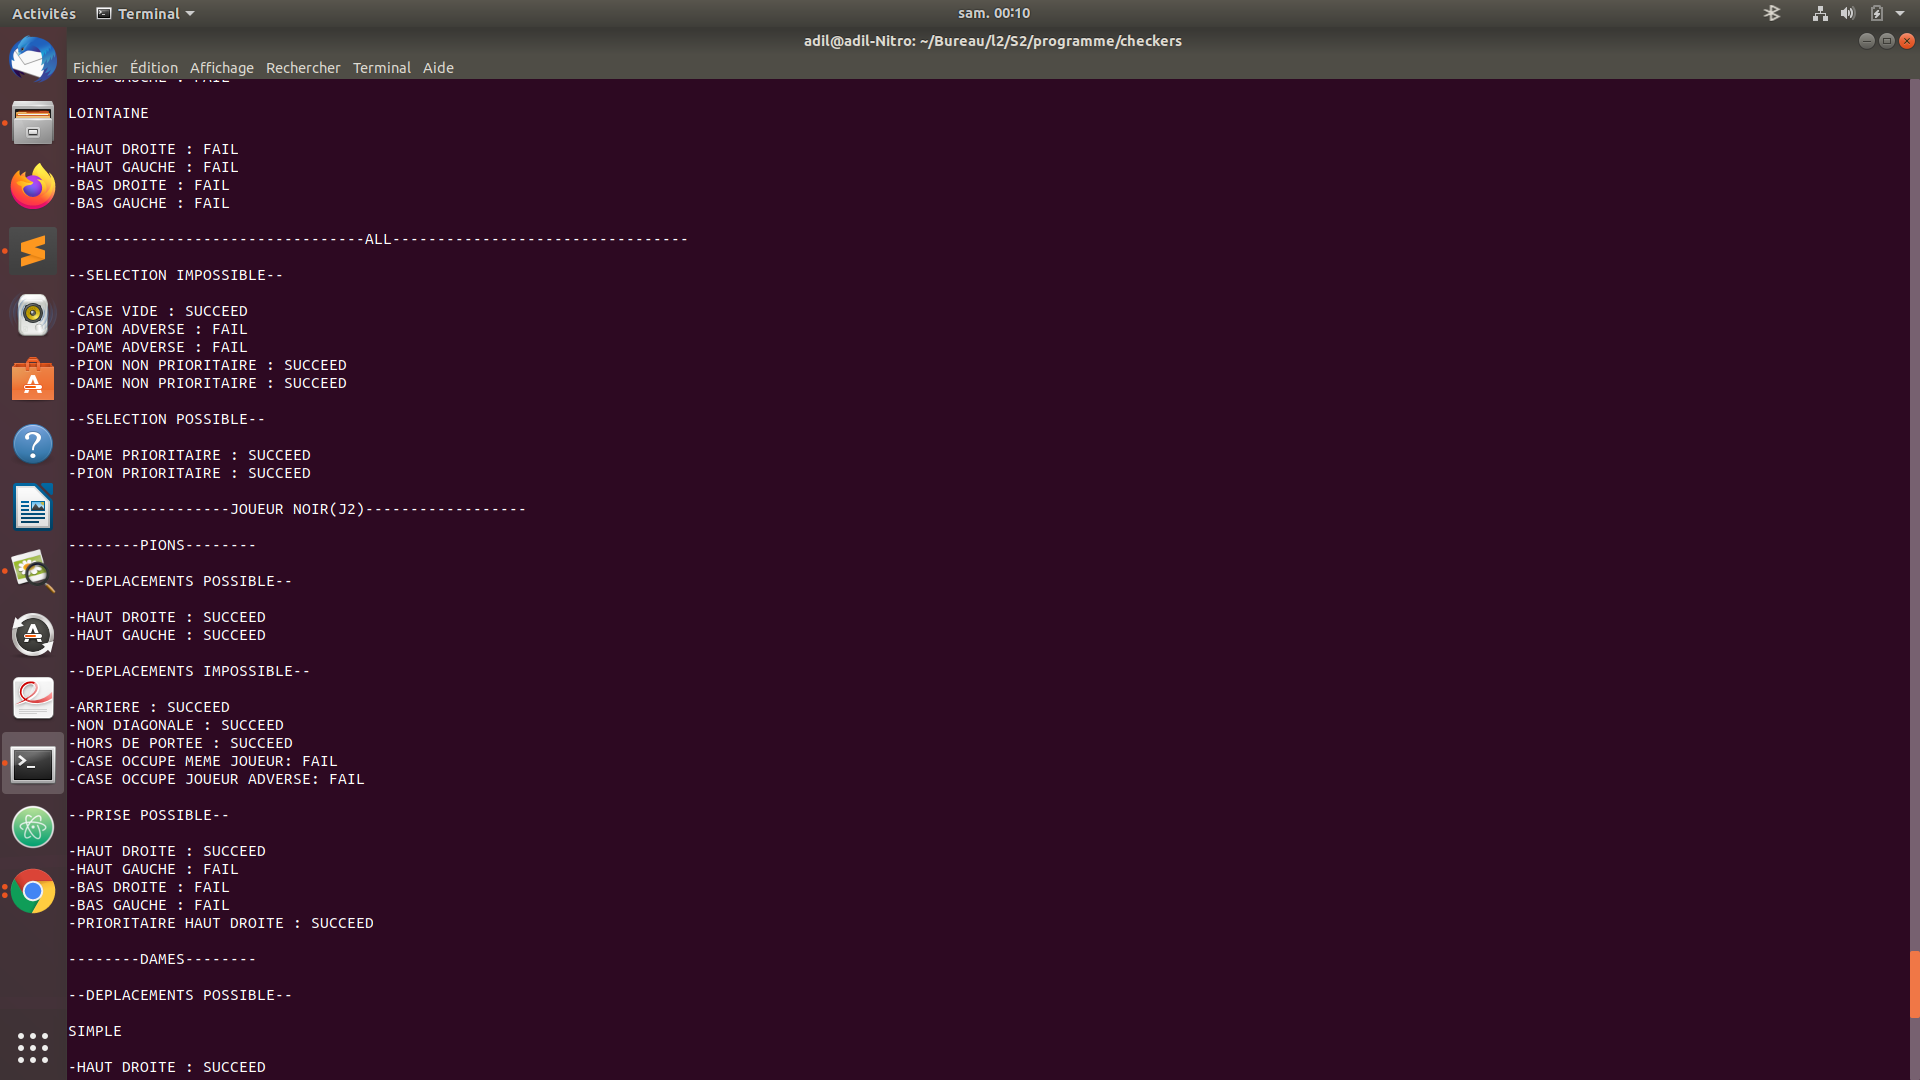
\includegraphics[width = 8cm, height = 5cm]{TestEchoue2.png}
\bigbreak
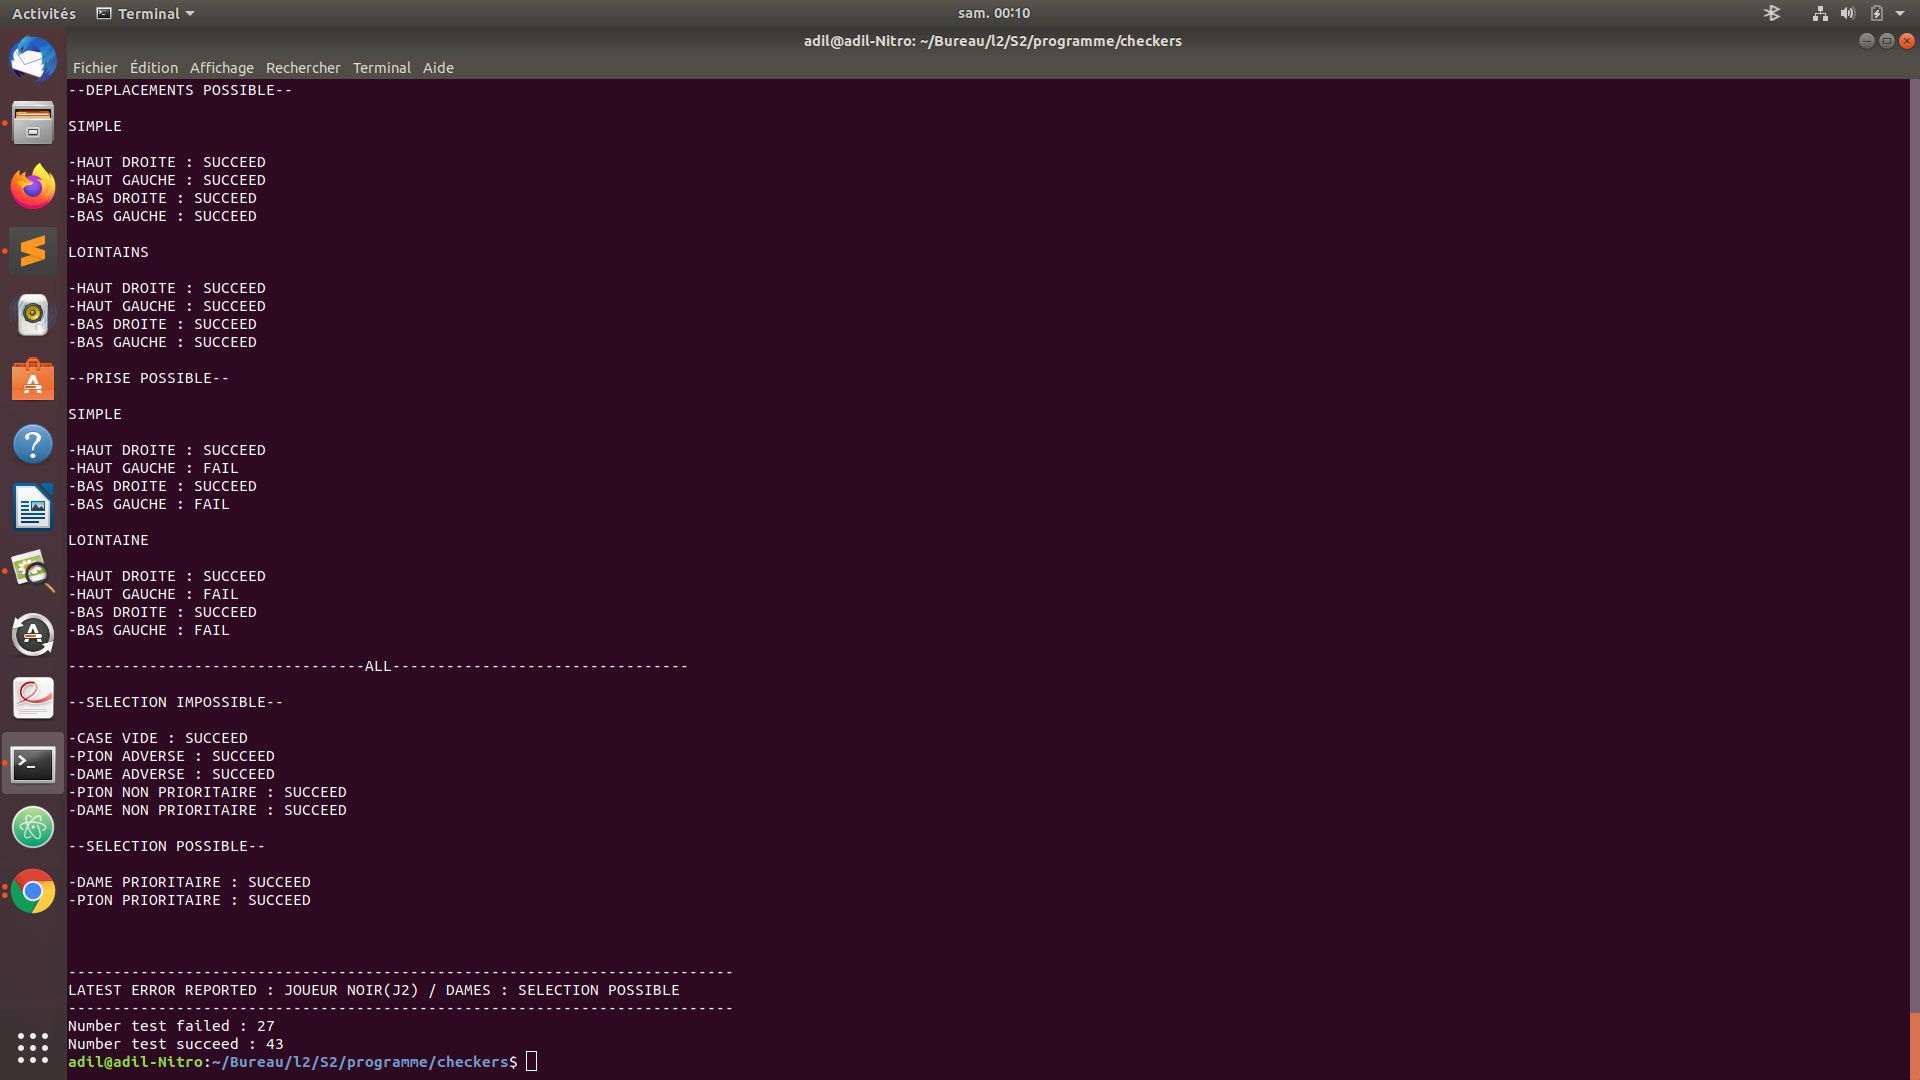
\includegraphics[width = 8cm, height = 5cm]{TestEchoue3.png}

\bigbreak

\begin{verbatim}

Comme vous pouvez le voir, notre programme passe bien les 70 tests sans erreurs.

\end{verbatim}

\large\bf{Test reussis : }
\bigbreak

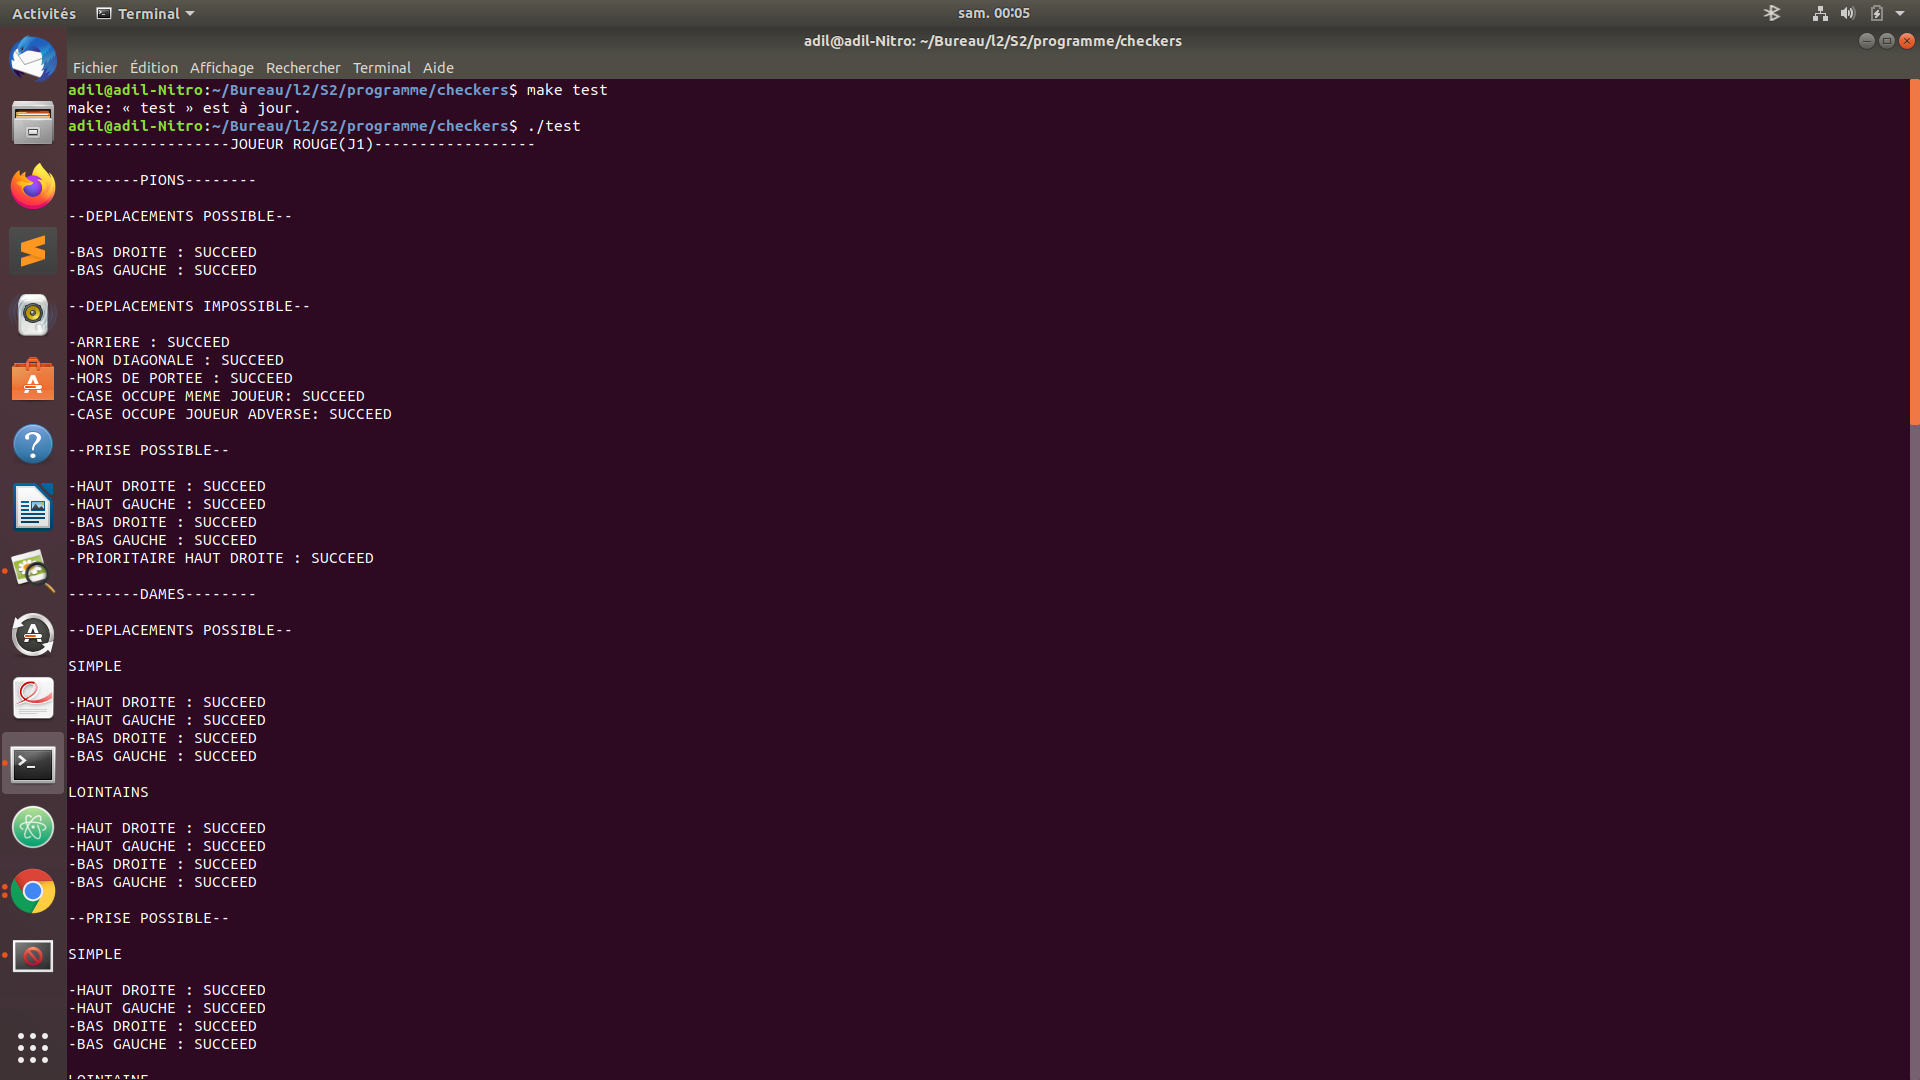
\includegraphics[width = 8cm, height = 5cm]{TestReussi1.png}
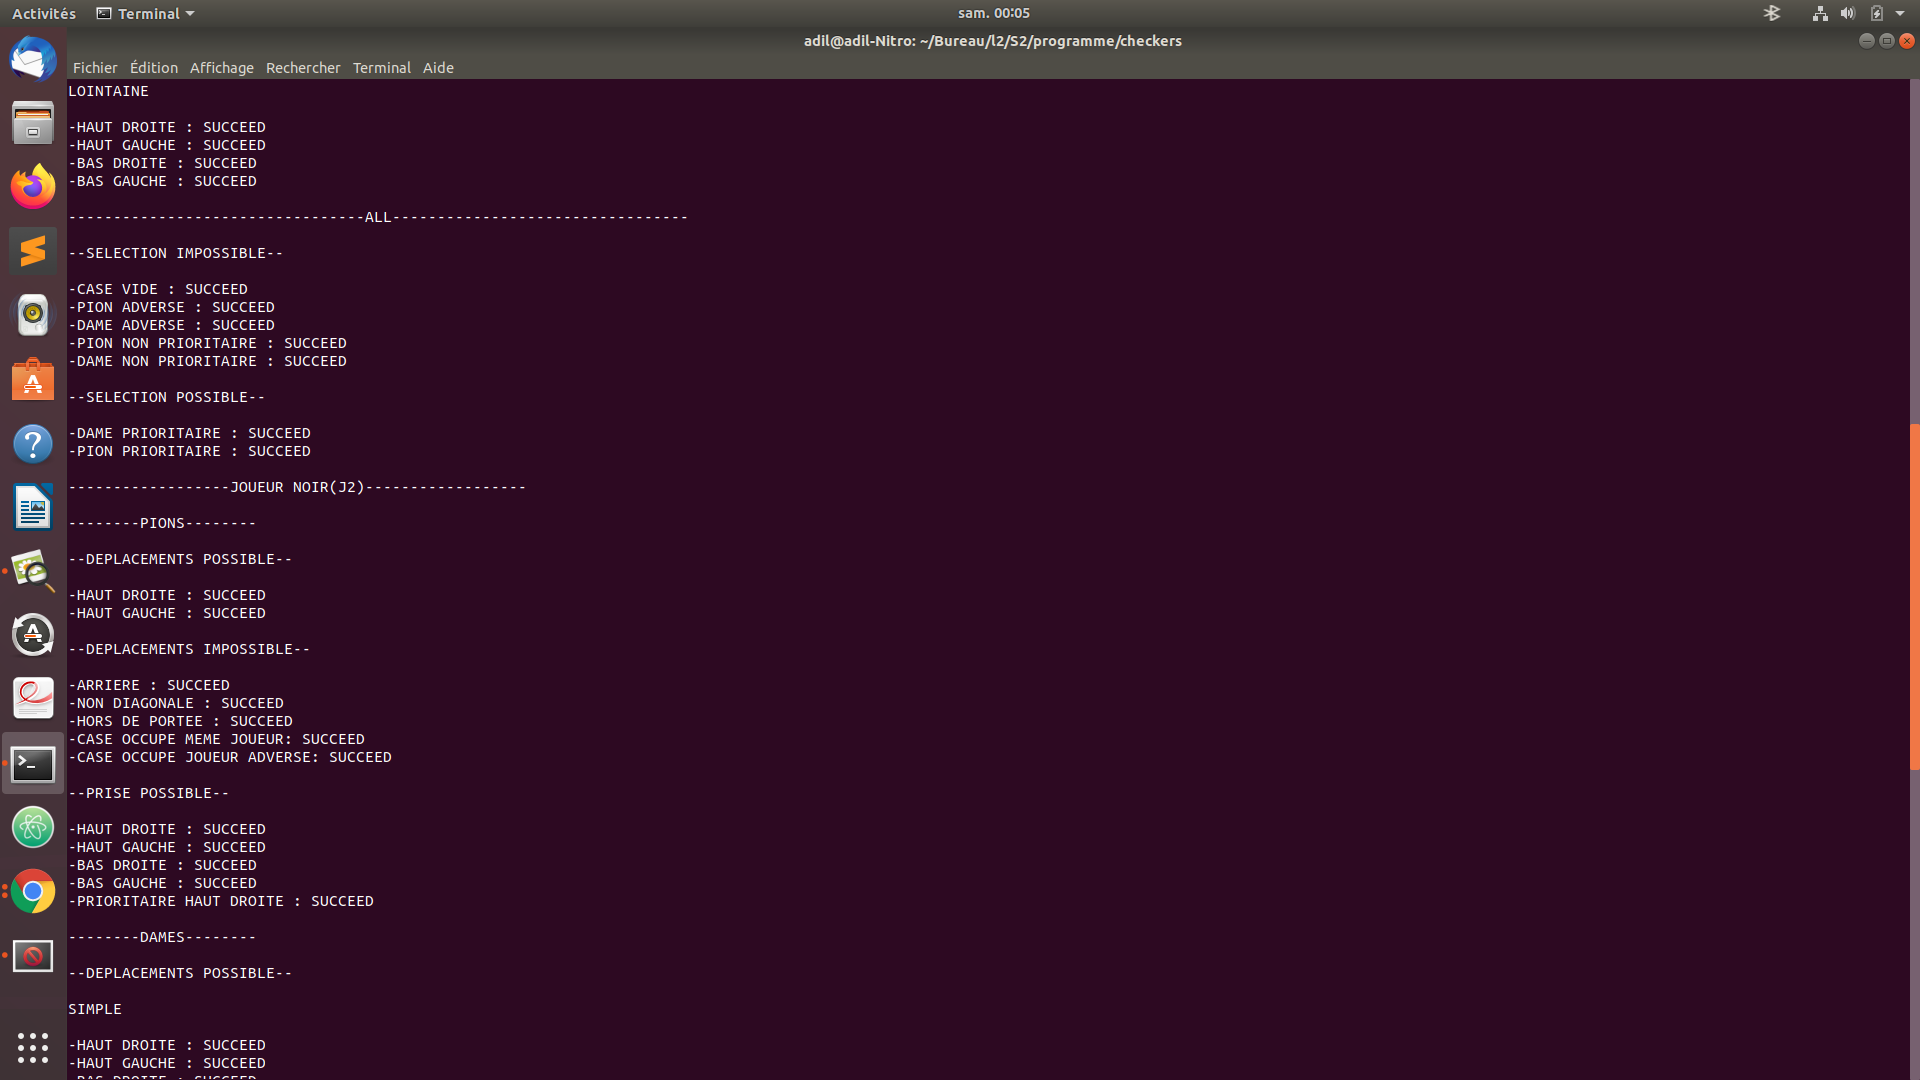
\includegraphics[width = 8cm, height = 5cm]{TestReussi2.png}
\bigbreak
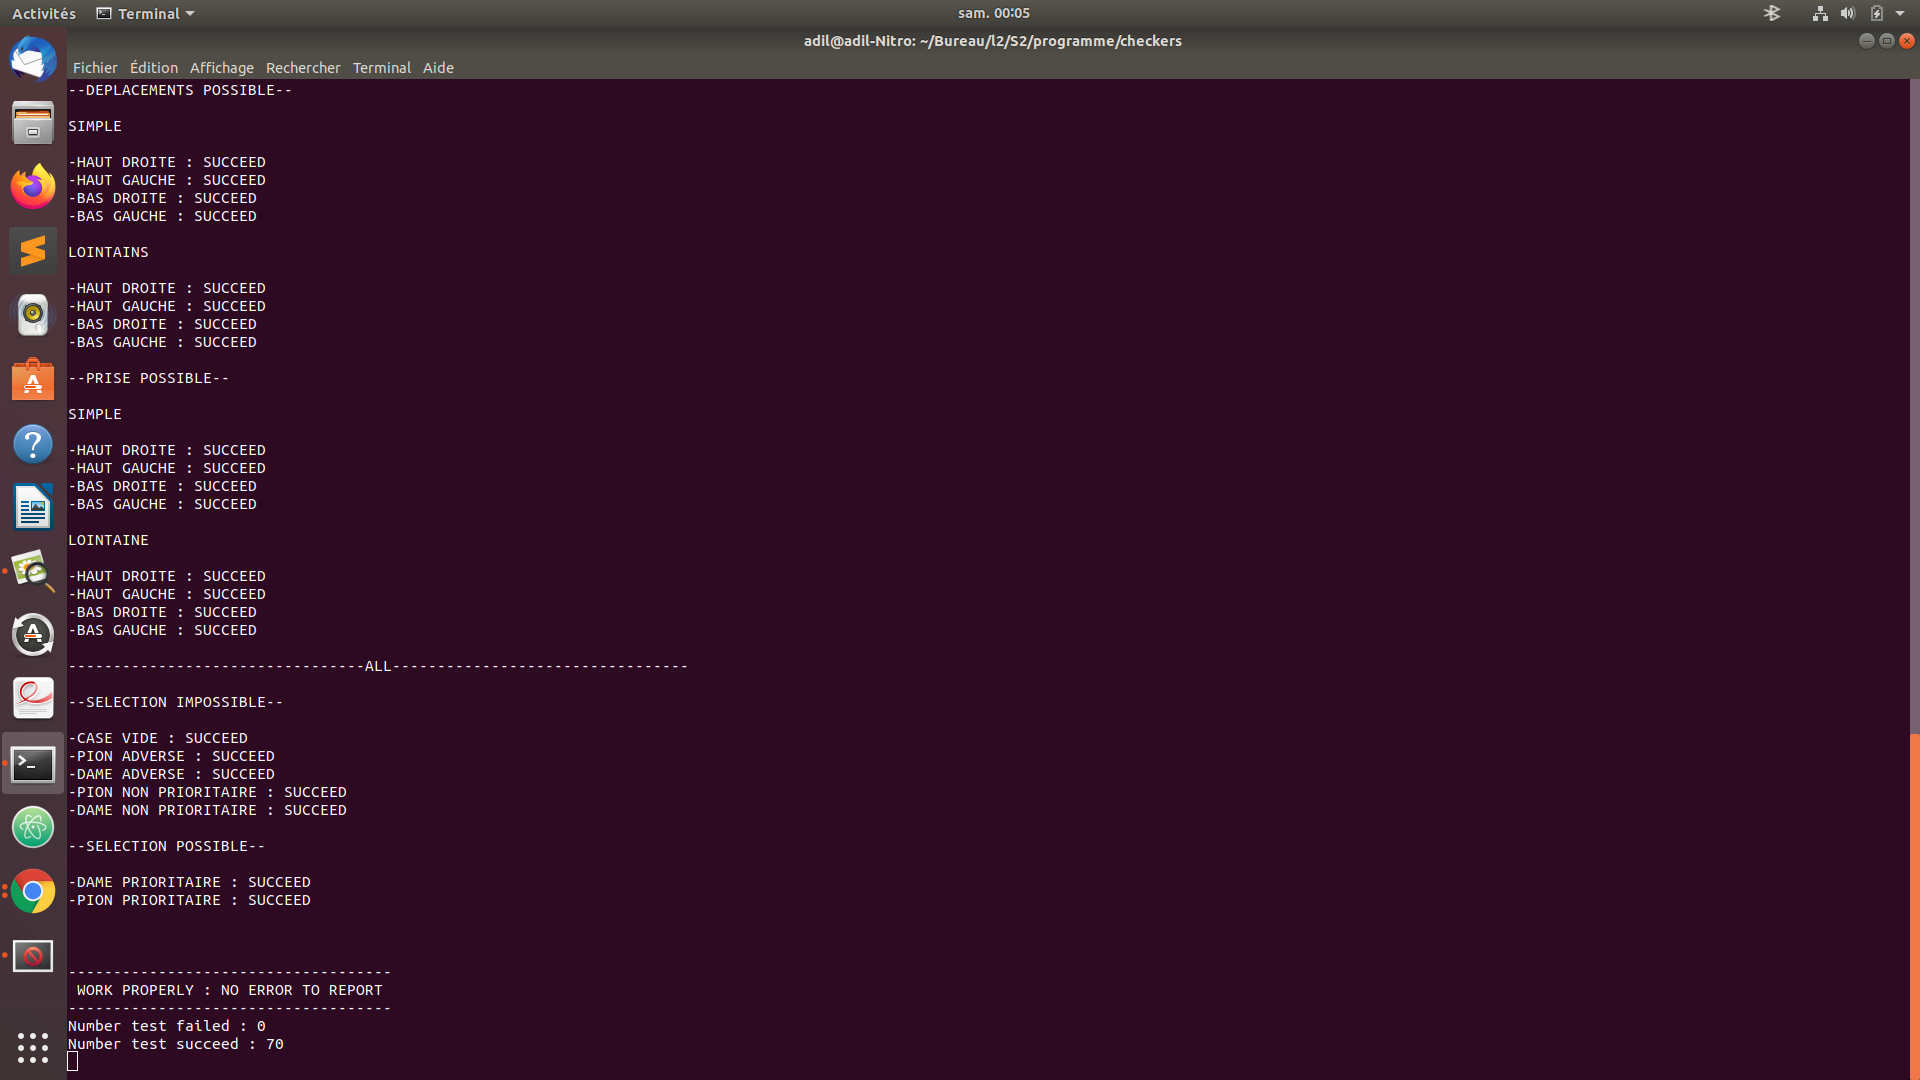
\includegraphics[width = 8cm, height = 5cm]{TestReussi3.png}

\end{document}